%!TeX program = xelatex
\documentclass[10pt,usenames,dvipsnames]{beamer}

% https://github.com/matze/mtheme
\usetheme[progressbar=frametitle]{metropolis}
\usepackage{appendixnumberbeamer}

% Install with fira fonts: 
%   sudo pacman -S ttf-fira-code ttf-fira-mono ttf-fira-sans

\usepackage{booktabs}
\usepackage[scale=2]{ccicons}

\usepackage{pgfplots}
\usepgfplotslibrary{dateplot}

\usepackage{xspace}
\newcommand{\themename}{\textbf{\textsc{metropolis}}\xspace}

\newcommand\blfootnote[1]{%
\begingroup
\renewcommand\thefootnote{}\footnote{#1}%
\addtocounter{footnote}{-1}%
\endgroup
}

\usepackage{xcolor-material} % https://ctan.org/pkg/xcolor-material
\usepackage{tikz}
\usetikzlibrary{fit}					% fitting shapes to coordinates
\usetikzlibrary{backgrounds}	% drawing the background after the foreground
\usetikzlibrary{calc, arrows, fit, positioning, patterns, decorations.pathreplacing, shapes}
\usetikzlibrary{shadows}
\usepackage{xifthen}
\usetikzlibrary{arrows.meta}
\usepackage{smartdiagram} % used in the applications slide

\tikzstyle{var}=[circle,
                 thick,
                 draw=black!100,
                 font=\small,
                ]

\tikzstyle{bag}=[circle,
                 ultra thick,
                 draw=black!100,
                 font=\small,
                ]

\tikzstyle{hsepset}=[rectangle,
                     minimum width=1.3cm,
                     draw=black!100,
                     font=\small,
                    ]

\tikzstyle{vsepset}=[rectangle,
                     minimum width=1.3cm,
                     draw=black!100,
                     rotate=90,
                     font=\small,
                    ]

\tikzstyle{msgcircle}=[shape=circle,
                       draw,
                       inner sep=0pt,
                       minimum size=4mm,
                       font=\scriptsize,
                      ]

\tikzstyle{roundrect}=[shape=rectangle,
                       draw,
                       rounded corners,
                       inner sep=7pt,
                       minimum width=22mm,
                       minimum height=9mm,
                       font=\footnotesize,
                       %thick,
                      ]

% Used in the factor graph
\tikzstyle{box} = [draw, minimum size=7.0mm]
\tikzstyle{line} = [draw, -latex,>=latex]

\newcommand{\msgcircle}[7]{
  % Circle left arrow down
  \ifthenelse{\isin{#1}{left} \AND \isin{#2}{down}}{
    \coordinate (anchor) at ($({#3})!{#5}!({#4})$);
    \node[color={#7}, msgcircle, xshift=-5.0mm] at (anchor) {#6};
    \node[color={#7}, xshift=-1.5mm] at (anchor) {$\Big\downarrow$};
  }{}
  % Circle right arrow down
  \ifthenelse{\isin{#1}{right} \AND \isin{#2}{down}}{
    \coordinate (anchor) at ($({#3})!{#5}!({#4})$);
    \node[color={#7}, msgcircle ,xshift=5.0mm] at (anchor) {#6};
    \node[color={#7}, xshift=1.7mm] at (anchor) {$\Big\downarrow$};
  }{}

  % Circle down arrow right
  \ifthenelse{\isin{#1}{down} \AND \isin{#2}{right}}{
    \coordinate (anchor) at ($({#3})!{#5}!({#4})$);
    \node[color={#7}, msgcircle, yshift=-5.0mm] at (anchor) {#6};
    \node[color={#7}, yshift=-1.7mm, rotate=90] at (anchor) {$\Big\downarrow$};
  }{}
  % Circle up arrow right
  \ifthenelse{\isin{#1}{up} \AND \isin{#2}{right}}{
    \coordinate (anchor) at ($({#3})!{#5}!({#4})$);
    \node[color={#7}, msgcircle, yshift=5.0mm] at (anchor) {#6};
    \node[color={#7}, yshift=1.5mm, rotate=90] at (anchor) {$\Big\downarrow$};
  }{}

  % Circle down arrow left
  \ifthenelse{\isin{#1}{down} \AND \isin{#2}{left}}{
    \coordinate (anchor) at ($({#3})!{#5}!({#4})$);
    \node[color={#7}, msgcircle, yshift=-5.0mm] at (anchor) {#6};
    \node[color={#7}, yshift=-1.7mm, rotate=-90] at (anchor) {$\Big\downarrow$};
  }{}
  % Circle up arrow left
  \ifthenelse{\isin{#1}{up} \AND \isin{#2}{left}}{
    \coordinate (anchor) at ($({#3})!{#5}!({#4})$);
    \node[color={#7}, msgcircle, yshift=5.0mm] at (anchor) {#6};
    \node[color={#7}, yshift=1.5mm, rotate=-90] at (anchor) {$\Big\downarrow$};
  }{}

  % Circle left arrow up
  \ifthenelse{\isin{#1}{left} \AND \isin{#2}{up}}{
    \coordinate (anchor) at ($({#3})!{#5}!({#4})$);
    \node[color={#7}, msgcircle, xshift=-5.0mm] at (anchor) {#6};
    \node[color={#7}, xshift=-1.5mm, rotate=180] at (anchor) {$\Big\downarrow$};
  }{}
  % Circle right arrow up
  \ifthenelse{\isin{#1}{right} \AND \isin{#2}{up}}{
    \coordinate (anchor) at ($({#3})!{#5}!({#4})$);
    \node[color={#7}, msgcircle, xshift=5.0mm] at (anchor) {#6};
    \node[color={#7}, xshift=1.7mm, rotate=180] at (anchor) {$\Big\downarrow$};
  }{}
}

% https://tex.stackexchange.com/questions/39553/how-can-i-show-coordinates-by-grid-in-tikz-automatically
\makeatletter
\def\grd@save@target#1{%
  \def\grd@target{#1}}
\def\grd@save@start#1{%
  \def\grd@start{#1}}
\tikzset{
  grid with coordinates/.style={
    to path={%
      \pgfextra{%
        \edef\grd@@target{(\tikztotarget)}%
        \tikz@scan@one@point\grd@save@target\grd@@target\relax
        \edef\grd@@start{(\tikztostart)}%
        \tikz@scan@one@point\grd@save@start\grd@@start\relax
        \draw[minor help lines] (\tikztostart) grid (\tikztotarget);
        \draw[major help lines] (\tikztostart) grid (\tikztotarget);
        \grd@start
        \pgfmathsetmacro{\grd@xa}{\the\pgf@x/1cm}
        \pgfmathsetmacro{\grd@ya}{\the\pgf@y/1cm}
        \grd@target
        \pgfmathsetmacro{\grd@xb}{\the\pgf@x/1cm}
        \pgfmathsetmacro{\grd@yb}{\the\pgf@y/1cm}
        \pgfmathsetmacro{\grd@xc}{\grd@xa + \pgfkeysvalueof{/tikz/grid with coordinates/major step}}
        \pgfmathsetmacro{\grd@yc}{\grd@ya + \pgfkeysvalueof{/tikz/grid with coordinates/major step}}
        \foreach \x in {\grd@xa,\grd@xc,...,\grd@xb}
        \node[anchor=north] at (\x,\grd@ya) {\tiny{\pgfmathprintnumber{\x}}};
        \foreach \y in {\grd@ya,\grd@yc,...,\grd@yb}
        \node[anchor=east] at (\grd@xa,\y) {\tiny{\pgfmathprintnumber{\y}}};
      }
    }
  },
  minor help lines/.style={
    help lines,
    step=\pgfkeysvalueof{/tikz/grid with coordinates/minor step}
  },
  major help lines/.style={
    help lines,
    line width=\pgfkeysvalueof{/tikz/grid with coordinates/major line width},
    step=\pgfkeysvalueof{/tikz/grid with coordinates/major step}
  },
  grid with coordinates/.cd,
  minor step/.initial=0,
  major step/.initial=1,
  major line width/.initial=0.5pt,
}
\makeatother


% https://tex.stackexchange.com/questions/82413/drawing-a-node-surrounding-arbitrarily-places-nodes
% https://tex.stackexchange.com/questions/27171/padded-boundary-of-convex-hull#27185
\usetikzlibrary{calc,trees}

\newcommand{\convexpath}[2]{
  [   
  create hullnodes/.code={
    \global\edef\namelist{#1}
    \foreach [count=\counter] \nodename in \namelist {
      \global\edef\numberofnodes{\counter}
      \node at (\nodename) [draw=none,name=hullnode\counter] {};
    }
    \node at (hullnode\numberofnodes) [name=hullnode0,draw=none] {};
    \pgfmathtruncatemacro\lastnumber{\numberofnodes+1}
    \node at (hullnode1) [name=hullnode\lastnumber,draw=none] {};
  },
  create hullnodes
  ]
  ($(hullnode1)!#2!-90:(hullnode0)$)
  \foreach [
  evaluate=\currentnode as \previousnode using \currentnode-1,
  evaluate=\currentnode as \nextnode using \currentnode+1
  ] \currentnode in {1,...,\numberofnodes} {
    -- ($(hullnode\currentnode)!#2!-90:(hullnode\previousnode)$)
    let \p1 = ($(hullnode\currentnode)!#2!-90:(hullnode\previousnode) - (hullnode\currentnode)$),
    \n1 = {atan2(\y1,\x1)},
    \p2 = ($(hullnode\currentnode)!#2!90:(hullnode\nextnode) - (hullnode\currentnode)$),
    \n2 = {atan2(\y2,\x2)},
    \n{delta} = {-Mod(\n1-\n2,360)}
    in 
    {arc [start angle=\n1, delta angle=\n{delta}, radius=#2]}
  }
  -- cycle
}

% A command to create an overview of the junction tree algorithm
% Takes 2 parameters:
% 1. Name of the section to highlight
% 2. Name of the subsection to highlight
\newcommand{\pptc}[2]{

  \tikzset {
    every node/.style={node distance=1.4cm},
    mybox/.style= {
      rectangle,rounded corners,drop shadow,minimum height=0.7cm,font=\small,
      minimum width=\columnwidth*0.8,align=center,fill=white,draw=gray,line width=1pt
    },
    myarrow/.style= { draw=gray,line width=2pt,-stealth },
    mylabel/.style={text=black,right,xshift=2mm,text width=4.2cm,font=\small},
    surrbox/.style={thick,draw=black,rounded corners=2mm},
    surrboxlabel/.style={anchor=center,rotate=90,yshift=3mm,font=\small},
  }

  \begin{tikzpicture}

    \ifthenelse{\equal{#1}{Probabilistic Graphical Model}}{
      \node[mybox] (pgm) {\textbf{\alert{Probabilistic Graphical Model}}};
    }{
      \node[mybox] (pgm) {Probabilistic Graphical Model};
    }

    \ifthenelse{\equal{#1}{Junction Tree} }{
      \node[mybox,below=of pgm,yshift=-0.4cm] (jts) {\textbf{\alert{Junction Tree}}};
    }{
      \node[mybox,below=of pgm,yshift=-0.4cm] (jts) {Junction Tree};
    }

    \ifthenelse{\equal{#1}{Inconsistent Junction Tree}}{
      \node[mybox,below=of jts] (ijt) {\textbf{\alert{Inconsistent Junction Tree}}};
    }{
      \node[mybox,below=of jts] (ijt) {Inconsistent Junction Tree};
    }

    \ifthenelse{\equal{#1}{Consistent Junction Tree}}{
      \node[mybox,below=of ijt,yshift=0.4cm] (cjt) {\textbf{\alert{Consistent Junction Tree}}};
    }{
      \node[mybox,below=of ijt,yshift=0.4cm] (cjt) {Consistent Junction Tree};
    }

    \ifthenelse{\equal{#1}{Consistent Junction Tree}}{
      \node[mybox,below=of ijt,yshift=0.4cm] (cjt) {\textbf{\alert{Consistent Junction Tree}}};
    }{
      \node[mybox,below=of ijt,yshift=0.4cm] (cjt) {Consistent Junction Tree};
    }

    \node[below=of cjt] (mar) {$P(V \mid \bm{E=e})$};

    \draw[myarrow] (pgm) -- (jts);
    \draw[myarrow] (jts) -- (ijt);
    \draw[myarrow] (ijt) -- (cjt);
    \draw[myarrow] (cjt) -- (mar);

    %-------------------------------------------------------------------

    \ifthenelse{\equal{#2}{Moralization}}{
      \path (pgm) -- node[mylabel] (gt) {\textbf{\alert{1. Moralization}}\\2. Triangulation\\3. Connection of clusters} (jts);
    }{}

    \ifthenelse{\equal{#2}{Triangulation}}{
      \path (pgm) -- node[mylabel] (gt) {1. Moralization\\\textbf{\alert{2. Triangulation}}\\3. Connection of clusters} (jts);
    }{}

    \ifthenelse{\equal{#2}{Connection of clusters}}{
      \path (pgm) -- node[mylabel] (gt) {1. Moralization\\2. Triangulation\\\textbf{\alert{3. Connection of clusters}}} (jts);
    }{}

    \ifthenelse{\not \equal{#2}{Moralization} \AND \not \equal{#2}{Triangulation} \AND \not \equal{#2}{Connection of clusters}}{
      \path (pgm) -- node[mylabel] (gt) {1. Moralization\\2. Triangulation\\3. Connection of clusters} (jts);
    }{}

    %-------------------------------------------------------------------

    \ifthenelse{\equal{#2}{Initialization}}{
      \path (jts) -- node[mylabel] (ini) {\textbf{\alert{1. Initialization}}\\2. Observation entry} (ijt);
    }{}

    \ifthenelse{\equal{#2}{Observation entry}}{
      \path (jts) -- node[mylabel] (ini) {1. Initialization\\\textbf{\alert{2. Observation entry}}} (ijt);
    }{}

    \ifthenelse{\not \equal{#2}{Initialization} \AND \not \equal{#2}{Observation entry}}{
      \path (jts) -- node[mylabel] (ini) {1. Initialization\\2. Observation entry} (ijt);
    }{}

    %-------------------------------------------------------------------

    \ifthenelse{\equal{#2}{Propagation}}{
      \path (ijt) -- node[mylabel] (pro) {\textbf{\alert{Propagation}}} (cjt);
    }{
      \path (ijt) -- node[mylabel] (pro) {Propagation} (cjt);
    }

    %-------------------------------------------------------------------

    \ifthenelse{\equal{#2}{Marginalization}}{
      \path (cjt) -- node[mylabel] (mar-nor) {\textbf{\alert{1. Marginalization}}\\2. Normalization} (mar);
    }{}

    \ifthenelse{\equal{#2}{Normalization}}{
      \path (cjt) -- node[mylabel] (mar-nor) {1. Marginalization\\\textbf{\alert{2. Normalization}}} (mar);
    }{}

    \ifthenelse{\not \equal{#2}{Marginalization} \AND \not \equal{#2}{Normalization}}{
      \path (cjt) -- node[mylabel] (mar-nor) {1. Marginalization\\2. Normalization} (mar);
    }{}

  \end{tikzpicture}
}


\usepackage{pgfplots}
\pgfplotsset{compat=1.17}
\usepackage{bm} % used to for bold letters in math environments
\usepackage{circledsteps}
\usepackage{ulem} % used to strike out text
%\usepackage[table]{xcolor} % used for alternating row color

\definecolor{bblue}{HTML}{2B83BA}
\definecolor{ggreen}{HTML}{ABDDA4}
\definecolor{rred}{HTML}{D7191C}
\definecolor{yyellow}{HTML}{FDAE61}

\colorlet{D}{MaterialGreen!40}
\colorlet{B}{MaterialCyan!40}
\colorlet{A}{MaterialOrange!40}
\colorlet{F}{MaterialRed!40}
\colorlet{C}{MaterialBlue!40}
\colorlet{E}{MaterialPurple!40}

\colorlet{BD}{GoogleBlue}
\colorlet{ABC}{GoogleGreen}
\colorlet{BCE}{GoogleYellow}
\colorlet{BEF}{GoogleRed}

% Source: https://www.quora.com/What-is-the-best-way-to-visualize-my-social-graph
\definecolor{MyGreen}{HTML}{669802}
\definecolor{MyBlue}{HTML}{046798}
\definecolor{MyOrange}{HTML}{FC6232}
\definecolor{MyCyan}{HTML}{8CB7CB}
\definecolor{MyPink}{HTML}{CE7295}
\definecolor{MyYellow}{HTML}{F19B3C}

\colorlet{mygray}{gray!30}

% \fbox tip:
% - https://tex.stackexchange.com/questions/119984/subfigures-side-by-side-with-captions
\usepackage{subcaption}

\usepackage{multirow}

\usepackage{booktabs}

% https://tex.stackexchange.com/a/43009/23046
\usepackage{mathtools} % provides absolute value \lvert and \rvert

% How to align images:
% - https://latex-beamer.com/tutorials/beamer-figure/
% - use `\hfill` and `\vfill`  before/after including the images

% How to scale a tikz image:
% - https://tex.stackexchange.com/q/98134/23046
% - `\resizebox` and `\scalebox`

% Beamer table - full guide with examples
% - https://latex-beamer.com/tutorials/beamer-table/

% https://tex.stackexchange.com/questions/82413/drawing-a1-node-surrounding-arbitrarily-places-nodes
% https://tex.stackexchange.com/questions/27171/padded-boundary-of-convex-hull#27185
\usetikzlibrary{calc,trees}

% https://openmetric.org/til/programming/latex-beamer-textblock-position/
\usepackage[absolute,overlay]{textpos}

%% Comment out to display a grid on each slide
%\usepackage[texcoord, grid,gridcolor=red!10,subgridcolor=green!10,gridunit=pt]{eso-pic}

% https://gist.github.com/andrejbauer/ac361549ac2186be0cdb
% https://tex.stackexchange.com/a/114227/23046
%\setbeameroption{hide notes} % Only slides
%\setbeameroption{show only notes} % Only notes
%\setbeameroption{show notes on second screen=right} % Both

%------------------------------------------------------------------------------
\title{The Junction Tree Algorithm}
\subtitle{A Visual Guide}
\date{\today}
%\date{}
\author{Martin Roa Villescas}
\institute{Eindhoven University of Technology}
\titlegraphic{\hfill
\includegraphics[height=0.8cm]{figures/tue_vector_logo.pdf}}

\begin{document}

%------------------------------------------------------------------------------
\maketitle

%-----------------------------------------------------------------------------
 \begin{frame}{Table of Contents}
   \setbeamertemplate{section in toc}[sections numbered]
   \tableofcontents[hideallsubsections]
 \end{frame}

%==============================================================================
\section{Problem Statement}
%==============================================================================

%------------------------------------------------------------------------------
\begin{frame}{What do these applications have in common?}
  \begin{textblock*}{10pt}(75pt,50pt)
    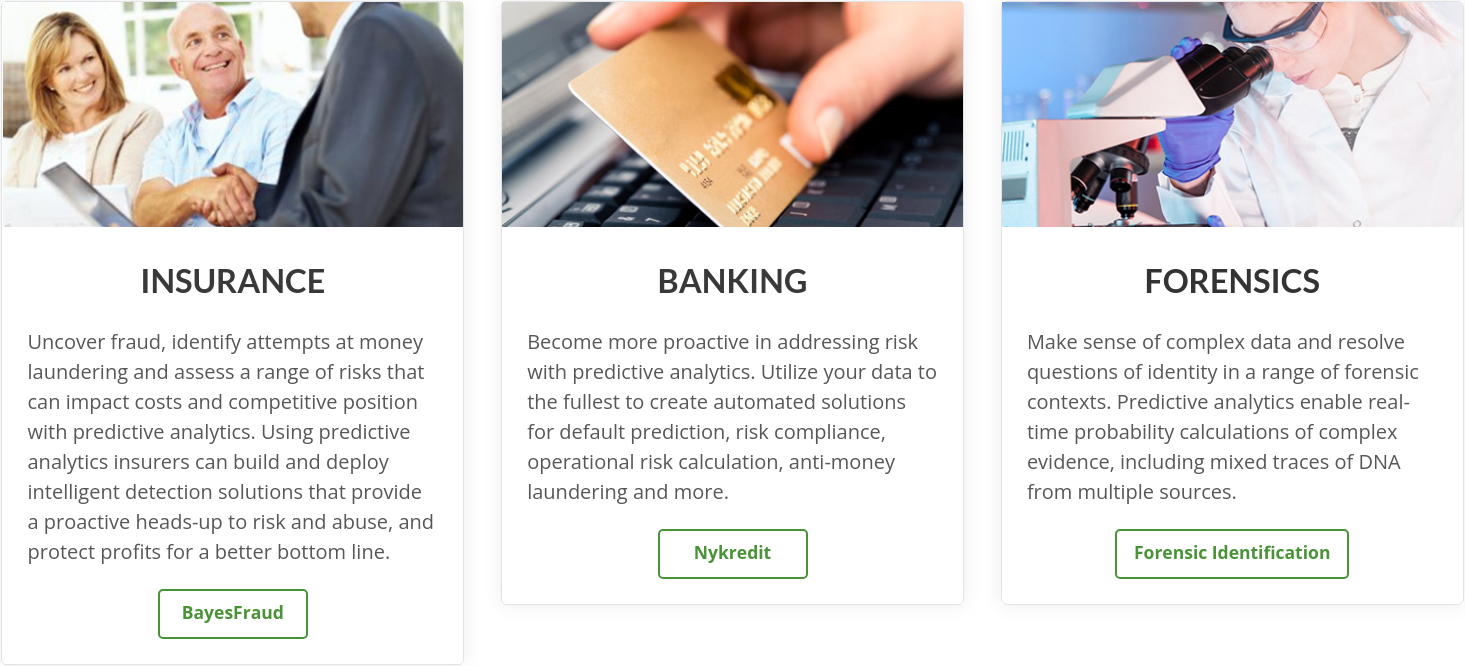
\includegraphics[width=215pt]{figures/hugin-expert/industry-applications-1.png}
  \end{textblock*}
  \begin{textblock*}{10pt}(75pt,150pt)
    
\includegraphics[width=215pt]{figures/hugin-expert/industry-applications-2.png}
  \end{textblock*}
\end{frame}

\note{ 
  BayesFraud: Our market leading solution provides insurers with advanced fraud
  detection capabilities for fast, proactive fraud detection. Discover how to
  protect your business and your customers from fraud by integrating the
  predictive computing power of BayesFraud in claims handling.
  BayesCredit: Using BayesCredit analytics, lending institutions can create
  customized solutions to analyze and identify credit default risk. Having the
  capability to accurately predict default risk enables lenders to reduce
  losses due to risk, and to grow their portfolios – and profits – with peace
  of mind. A major mortgage lending institution in Denmark has been using
  BayesCredit analytics for over a decade to assess risk and achieve risk
  compliance. 
  BayesAML: Anti-money laundering and anti-terror financing The BayesAML
  solution enables insurance companies, banks, casinos and other at-risk
  organizations to assess their customers, products and services according to
  risk. Implementing the real-time BayesAML tool, organizations can achieve a
  genuine risk-based approach to anti-money laundering that can assess
  customers and transactions and pinpoint those that are suspicious before
  money-laundering can be executed.
}

%------------------------------------------------------------------------------
% Set a white background
\setbeamercolor{normal text}{%
  fg=mDarkTeal,
  bg=black!0 % mrv
}

\begin{frame}{Complexity and Uncertainty}
  \centering
  \vspace{0.5cm} % manually adjust vertical positioning
  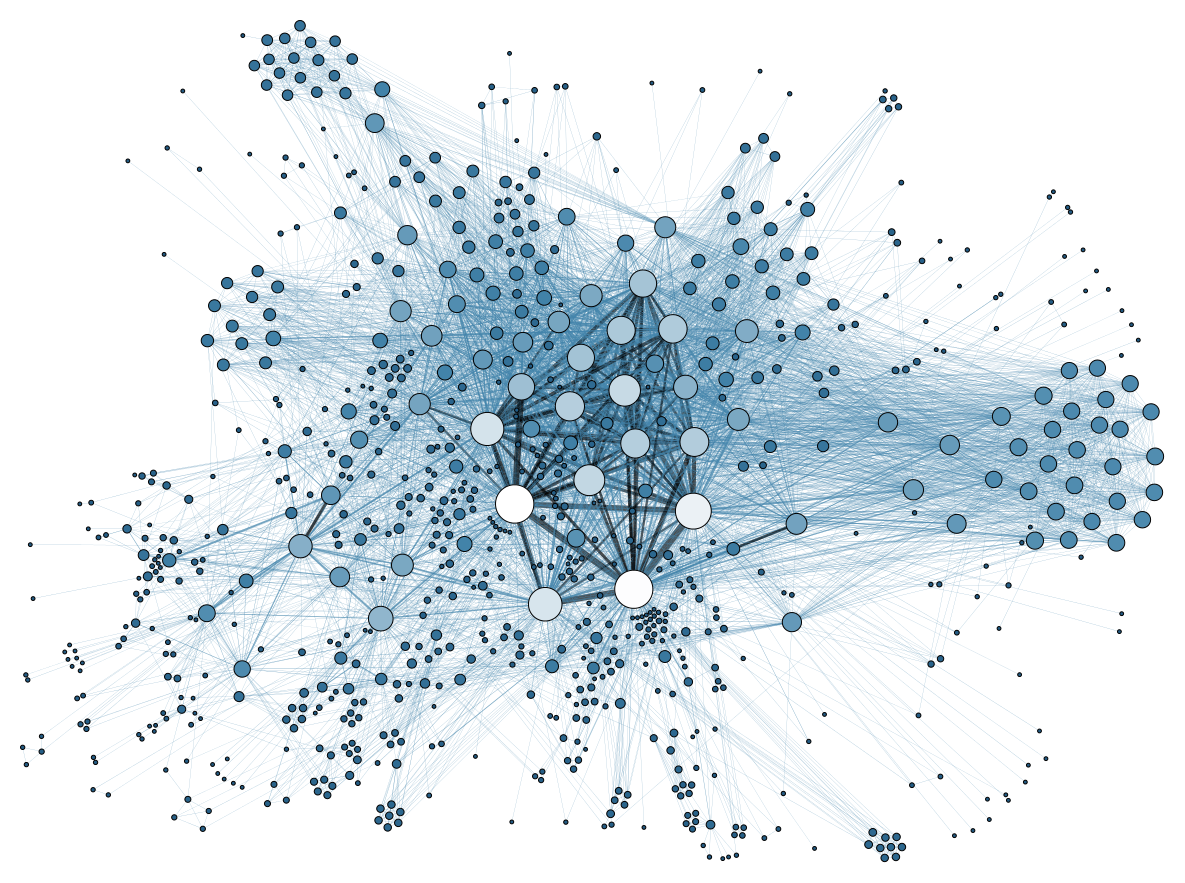
\includegraphics[scale=0.22]{figures/uncertainty-and-complexity/social-graph-network-visualization-by-martin-grandjean.png}
\end{frame}
\note{
  - There are two problems that occur often throughout applied mathematics and
  engineering: uncertainty and complexity.
  - Uncertainty arises because of several reasons: e.g. limitations on the
  availability of information, limitations in our ability to observe the world,
  limitations in our ability to model it.
  - On the other hand, complexity arises due to the fact that we are often
  trying to model a system that involves many variables that interact with each
  other.
}

%\begin{frame}{Uncertainty}
%  \centering
%  \vspace{0.5cm} % manually adjust vertical positioning
%  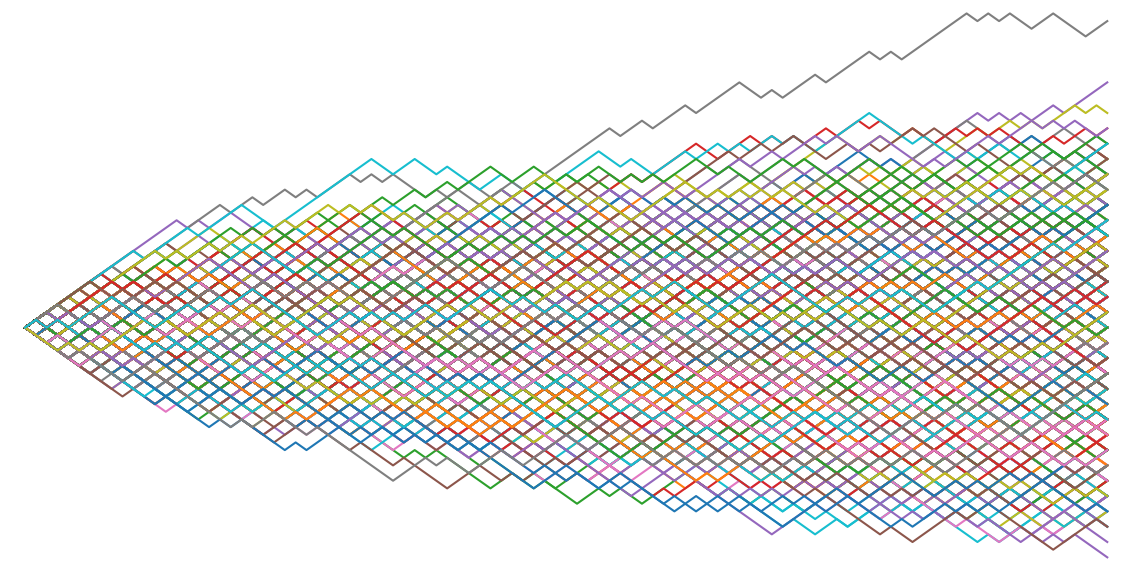
\includegraphics[scale=0.22]{figures/uncertainty-and-complexity/random-walks.png}
%\end{frame}

% Reset metropolis' background color 
\setbeamercolor{normal text}{%
  fg=mDarkTeal,
  bg=black!2
}

%==============================================================================
\section{Probabilistic Graphical Models}
%==============================================================================

%------------------------------------------------------------------------------
\begin{frame}{Probabilistic Graphical Models}
  \begin{figure}
    \centering
    \vspace{0.0cm} % manually adjust vertical positioning
    \scalebox{1.0}{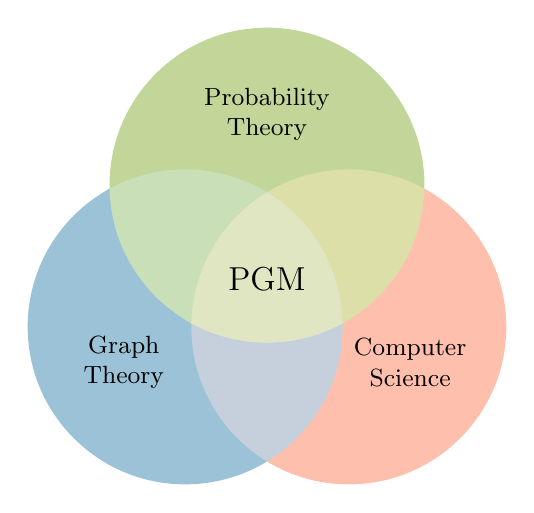
\begin{tikzpicture}

  \begin{scope}[blend group = soft light]
    \fill[MyGreen!40!white]   ( 90:1.2) circle (2);
    \fill[MyBlue!40!white]    (210:1.2) circle (2);
    \fill[MyOrange!40!white]  (330:1.2) circle (2);
  \end{scope}
  \node[font=\small,align=center] at (  90:2.1)   {Probability\\Theory};
  \node[font=\small,align=center] at ( 210:2.1)   {Graph\\Theory};
  \node[font=\small,align=center] at ( 330:2.1)   {Computer\\Science};
  \node[font=\large]                            {PGM};

\end{tikzpicture}

}
  \end{figure}
\end{frame}
% TODO: include a slide with with a real example (and a useful one) where the 
% Probabilistic graphical modeling framework would result useful.
\note{
  - Probability theory allows us to represent complex models compactly.
  - Probability theory allows us to update the knowledge based on new data
}

%------------------------------------------------------------------------------
\begin{frame}{Examples of PGMs}

  \begin{columns}

    % Column 1
    \begin{column}{0.5\textwidth}

      \begin{figure}
        \scalebox{0.7}{
\tikzset {
  myarrow/.style= {-{Stealth[scale=1.0]}},
}

\begin{tikzpicture}[]

  % The various elements are conveniently placed using a matrix:
  \matrix[row sep=0.05cm,column sep=0.5cm] {
    % First line
                                                &
                                                &
    \node (d) [var, minimum size=0.7cm] {$D$};  &
                                               \\
    % Second line
                                                &
    \node (b) [var, minimum size=0.7cm] {$B$};  &
                                                &
                                               \\
    % Third line
    \node (a) [var, minimum size=0.7cm] {$A$};  &
                                                &
                                                &
    \node (f) [var, minimum size=0.7cm] {$F$}; \\
    % Forth line
                                                &
    \node (c) [var, minimum size=0.7cm] {$C$};  &
    \node (e) [var, minimum size=0.7cm] {$E$};  &
                                               \\
  };

  \draw [myarrow] (a) edge (b);
  \draw [myarrow] (a) edge (c);
  \draw [myarrow] (b) edge (d);
  \draw [myarrow] (b) edge (f);
  \draw [myarrow] (c) edge (e);
  \draw [myarrow] (e) edge (f);

\end{tikzpicture}

}
        \caption{A Bayesian network}
      \end{figure}

      \begin{figure}
        \scalebox{0.7}{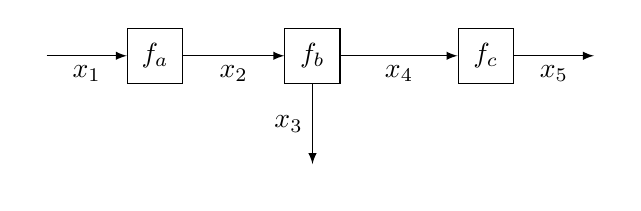
\begin{tikzpicture}[node distance=20mm,auto,>=stealth']
  \begin{scope}
    %\draw[style=dotted] (0,-10cm) grid[xstep=1cm, ystep=1cm] (12cm,6cm);

    \node[]at (0,0) (fl) {};
    \node[box, right of=fl, node distance=15mm] (fa) {$f_a$};
    \node[box, right of=fa] (fb) {$f_b$};
    \node[box, right of=fb,node distance=22mm] (fc) {$f_c$};
    \node[right of=fc, node distance=15mm] (fr) {};
    \node[below of=fb, node distance=15mm] (fd) {};

    \path[line] (fl) edge[->] node[anchor=north]{$x_1$} (fa);
    \path[line] (fa) edge[->] node[anchor=north]{$x_2$} (fb);
    \path[line] (fb) edge[->] node[anchor=north]{$x_4$} (fc);
    \path[line] (fc) edge[->] node[anchor=north]{$x_5$} (fr);
    \path[line] (fb) edge[->] node[anchor=east]{$x_3$} (fd);

    %\draw[dashed,opacity=1] (-0.05,-0.5) rectangle (2.0,0.5);
    %\draw[dashed,opacity=1] (-0.2,-1.5) rectangle(4,1);

    %% \draw[dashed,opacity=0.3] (5,-0.5) rectangle (7,0.5);
    %\msgcircle{up}{right}{fa}{fb}{0.5}{$1$}{black};
    %\msgcircle{up}{right}{fb}{fc}{0.37}{$2$}{black};
    %\msgcircle{up}{left}{fb}{fc}{0.65}{$3$}{black};

  \end{scope}
\end{tikzpicture}

}
        \caption{A factor graph}
      \end{figure}

    \end{column}

    % Column 2    
    \begin{column}{0.5\textwidth}

      \begin{figure}
        \scalebox{0.7}{% https://tex.stackexchange.com/a/61814/23046
\tikzset {
  myarrow/.style= {-{Stealth[scale=1.0]}},
  mycircle/.style= {circle,draw=black,minimum size=0.7cm},
}

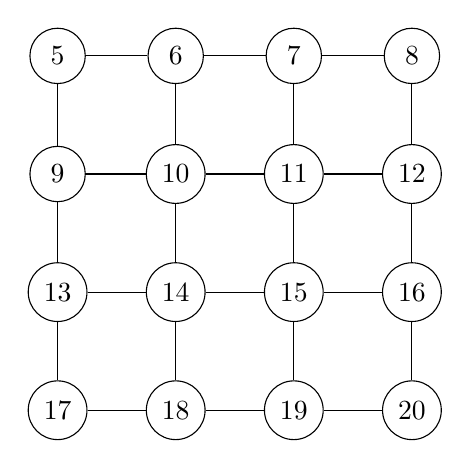
\begin{tikzpicture}[darkstyle/.style={circle,draw,minimum size=20}]
  \foreach \x in {0,...,3}
    \foreach \y in {0,...,3} 
        {\pgfmathtruncatemacro{\label}{\x - 4 *  \y +17}
        \node [darkstyle]  (\x\y) at (1.5*\x,1.5*\y) {\label};} 
  \foreach \x in {0,...,3}
    \foreach \y [count=\yi] in {0,...,2}  
      \draw (\x\y)--(\x\yi) (\y\x)--(\yi\x) ;
\end{tikzpicture}

}
        \caption{A Markov random field}
      \end{figure}

    \end{column}

  \end{columns}

\end{frame}


%%------------------------------------------------------------------------------
%% https://data-flair.training/blogs/bayesian-network-applications/
%\begin{frame}{Applications of Bayesian Inference}
%  \begin{figure}
%    \vspace{0.5cm} % manually adjust vertical positioning
%    \scalebox{0.55}{% A diagram of TeX engines
% Author: Stefan Kottwitz
% https://www.packtpub.com/hardware-and-creative/latex-cookbook

% Applications of Bayesian networks:
% https://data-flair.training/blogs/bayesian-network-applications/

\smartdiagramset{
  distance center/other bubbles=2.0cm,
  bubble center node size=4.6cm,
  bubble center node font=\large,
  bubble center node color=lightgray!80,
  bubble node size=2.8cm,
  bubble node font=\normalsize,
  set color list={
    MaterialRed,
    %MaterialPink,
    MaterialPurple,
    %MaterialDeepPurple,
    MaterialIndigo,
    %MaterialBlue,
    MaterialLightBlue,
    %MaterialCyan,
    MaterialTeal,
    %MaterialGreen,
    MaterialLightGreen,
    %MaterialLime,
    MaterialYellow,
    %MaterialAmber,
    MaterialOrange,
    MaterialDeepOrange,
    %MaterialBrown,
    %MaterialGrey,
    MaterialBlueGrey,
    %MaterialBlack,
  },
}

\smartdiagram[bubble diagram]{Bayesian Inference,
  Document\\Classification,
  Biomonitoring,
  Semantic\\Search,
  Spam\\Filter,
  System\\Biology,
  Medicine,
  Information\\Retrieval,
  Image\\Processing,
  Turbo\\Code
}

}
%  \end{figure}
%\end{frame}

%%------------------------------------------------------------------------------
%% https://data-flair.training/blogs/bayesian-network-applications/
%\begin{frame}{A General Framework}
%  \begin{figure}
%    \vspace{0.5cm} % manually adjust vertical positioning
%    \scalebox{0.8}{% A diagram of TeX engines
% Author: Stefan Kottwitz
% https://www.packtpub.com/hardware-and-creative/latex-cookbook

% Applications of Bayesian networks:
% https://data-flair.training/blogs/bayesian-network-applications/

\smartdiagramset{
  %distance center/other bubbles=2.0cm,
  %bubble center node size=4.6cm,
  %bubble center node font=\large,
  %bubble center node color=lightgray!80,
  %bubble node size=2.8cm,
  %bubble node font=\normalsize,
  set color list={
    MaterialRed,
    %MaterialPink,
    MaterialPurple,
    %MaterialDeepPurple,
    MaterialIndigo,
    %MaterialBlue,
    MaterialLightBlue,
    %MaterialCyan,
    MaterialTeal,
    %MaterialGreen,
    MaterialLightGreen,
    %MaterialLime,
    MaterialYellow,
    %MaterialAmber,
    MaterialOrange,
    MaterialDeepOrange,
    %MaterialBrown,
    %MaterialGrey,
    MaterialBlueGrey,
    %MaterialBlack,
  },
}

\smartdiagram[bubble diagram]{Probabilistic\\Graphical\\Models,
  Mixture\\Models,
  Factor\\Analysis,
  Kalman\\Filters,
  Hidden\\Markov\\Models,
  Ising\\Models
}

}
%  \end{figure}
%\end{frame}
%\note{
%  - Many classical algorithms studied in fields such as statistics, systems
%  engineering, information theory, pattern recognition and statistical mechanics
%  are special cases of the general graphical model formalism – this slide shows
%  examples. (click)
%  - This has many advantages – in particular, specialized techniques that have
%  been developed in one field can be transferred between research communities and
%  exploited more widely.
%}

%==============================================================================
\section{Bayesian Inference}
%==============================================================================

%%------------------------------------------------------------------------------
%\begin{frame}{Bayesian Inference}
%  \begin{figure}
%    \vspace{0.5cm} % manually adjust vertical positioning
%    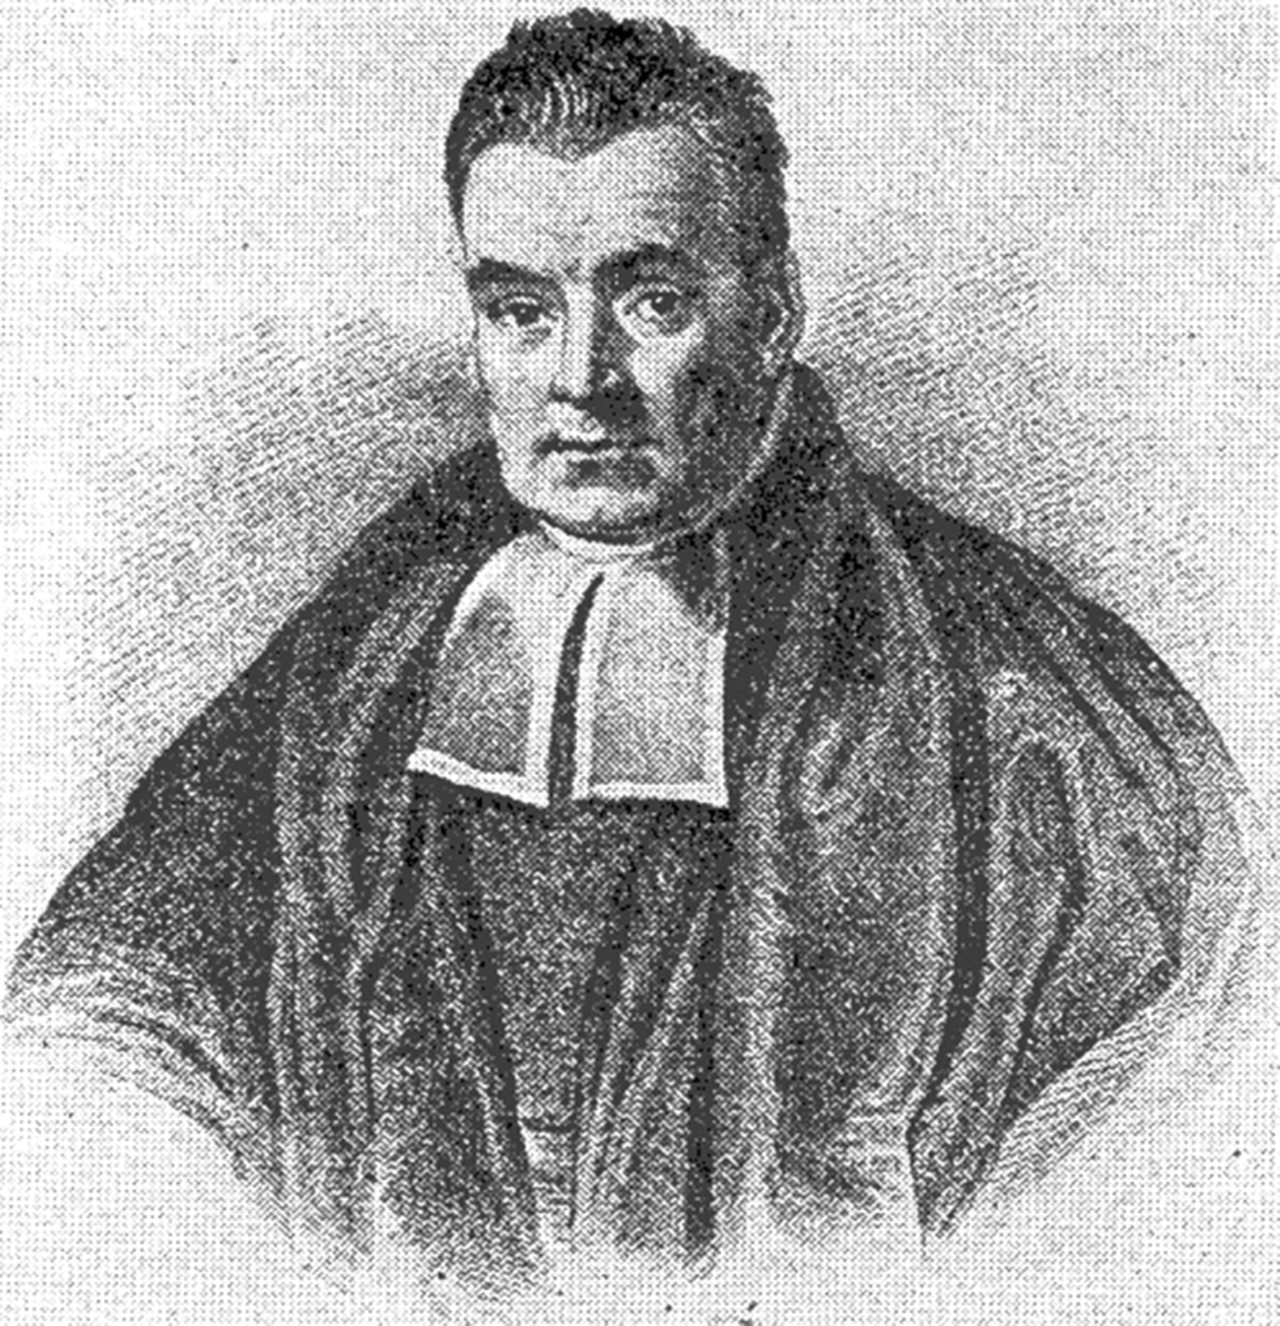
\includegraphics[scale=0.13]{figures/reverend-thomas-bayes.jpg}
%  \end{figure}
%\end{frame}

%------------------------------------------------------------------------------
\begin{frame}{The Inference Problem}
  \begin{small}
    \begin{quote} 
      Given a set of \textbf{random variables} $\mathcal{V}$ and their
      \textbf{joint distribution} $P(\mathcal{V})$,\\ compute one or more conditional
      distributions given observations.
    \end{quote}
  \end{small}
\end{frame}

%------------------------------------------------------------------------------
\begin{frame}{The Inference Problem}
  \begin{figure}
    \vspace{0.5cm} % manually adjust vertical positioning
    \scalebox{0.7}{\tikzset {
  every node/.style={node distance=20mm and 1.0mm},
  myroundbox/.style= {
    rectangle,rounded corners=3mm,drop shadow,minimum height=0.7cm,font=\small,
    minimum width=\columnwidth*0.28,align=center,fill=white,draw=black,
  },
  myrectbox/.style= {
    rectangle,drop shadow,minimum height=0.7cm,font=\small,
    minimum width=\columnwidth*0.28,align=center,fill=white,draw=black,
  },
  myarrow/.style={=black,-{Stealth[scale=1.0]},shorten >=2pt},
  mylabel/.style={text=black,right,xshift=2mm,text width=3.2cm,font=\small},
  surrbox/.style={thick,draw=black,rounded corners=2mm},
  surrboxlabel/.style={anchor=center,rotate=90,yshift=3mm,font=\small},
}

\begin{tikzpicture}

  %\draw[help lines] (0,0) grid (10,-7);

  % mrv: the "node distances" refer to the distance between the edge of a shape
  % to the edge of the other shape. That is why I use "ie_aux" and "mar_aux"
  % below: to have equal distances between nodes with respect to the center of
  % the shapes.

  % row 1
  \node[myroundbox] (rv) {Random Variables\\$\mathcal{V}$};
  \node[right=of rv](aux1) {};
  \node[right=of aux1,myroundbox] (jd) {Joint Distribution\\$P(\mathcal{V})$};
  \node[right=of jd](aux2) {};
  \node[right=of aux2,myroundbox] (e) {Evidence\\$\bm{E=e}$};
  \node[right=of e](aux3) {};
  \node[right=of aux3,myroundbox] (qv) {Query Variables\\$\bm{Q}$};
  % row 2
  \node[below=of aux2,myrectbox] (ie) {Inference Engine};
  \node[below=of aux2] (ie_aux) {};
  % row 3
  \node[below=of ie_aux,myroundbox] (mar) {$P(\bm{Q} \mid {\bf E=e})$};
  \node[below=of ie_aux] (mar_aux) {};
  % row 0
  \node[above=of aux2,yshift=-12mm] (in) {\textbf{Input}};
  % row 4
  \node[below=of mar_aux,yshift=10mm] (out) {\textbf{Output}};

  %% edges
  \draw[myarrow] (rv) -- (ie);
  \draw[myarrow] (jd) -- (ie);
  \draw[myarrow] (e)  -- (ie);
  \draw[myarrow] (qv) -- (ie);
  \draw[myarrow] (ie) -- (mar);

\end{tikzpicture}

}
  \end{figure}
  %\begin{footnotesize}
  %  \begin{columns}[T]
  %    % Column 1
  %    \begin{column}{0.5\textwidth}
  %      \textbf{Input}
  %      \begin{itemize}
  %        \item A set of random variables $\mathcal{V}$
  %        \item A joint probability distribution over $\mathcal{V}$
  %          \[ P(\mathcal{V}) = \prod_{V\in\mathcal{V}} P(V \mid pa(V)) \]
  %        \item An evidence assignment $\bm{E=e}$ 
  %        \item A set of query variables $\bm{Q}$ 
  %      \end{itemize}
  %    \end{column}
  %    % Column 2
  %    \begin{column}{0.5\textwidth}
  %      \textbf{Output}
  %      \begin{itemize} \item The conditional distribution $P(\bm{Q} \mid
  %        {\bf E=e})$ given the evidence $\bm{e}$ 
  %      \end{itemize}
  %    \end{column}
  %  \end{columns}
  %\end{footnotesize}
\end{frame}

%==============================================================================
\section{The Junction Tree Algorithm}
%==============================================================================

%------------------------------------------------------------------------------
\begin{frame}{The Junction Tree Algorithm}
    \begin{quote} 
      The \textbf{junction tree algorithm} is an efficient method to perform
      \textit{Bayesian inference} in general graphs.
    \end{quote}
\end{frame}

%------------------------------------------------------------------------------
% https://data-flair.training/blogs/bayesian-network-applications/
\begin{frame}{The Junction Tree Algorithm in Practice}
  \begin{textblock*}{10pt}(30pt,140pt)
    
\includegraphics[width=60pt]{figures/hugin-expert/hugin-expert.png}
  \end{textblock*}
  \begin{textblock*}{10pt}(120pt,50pt)
    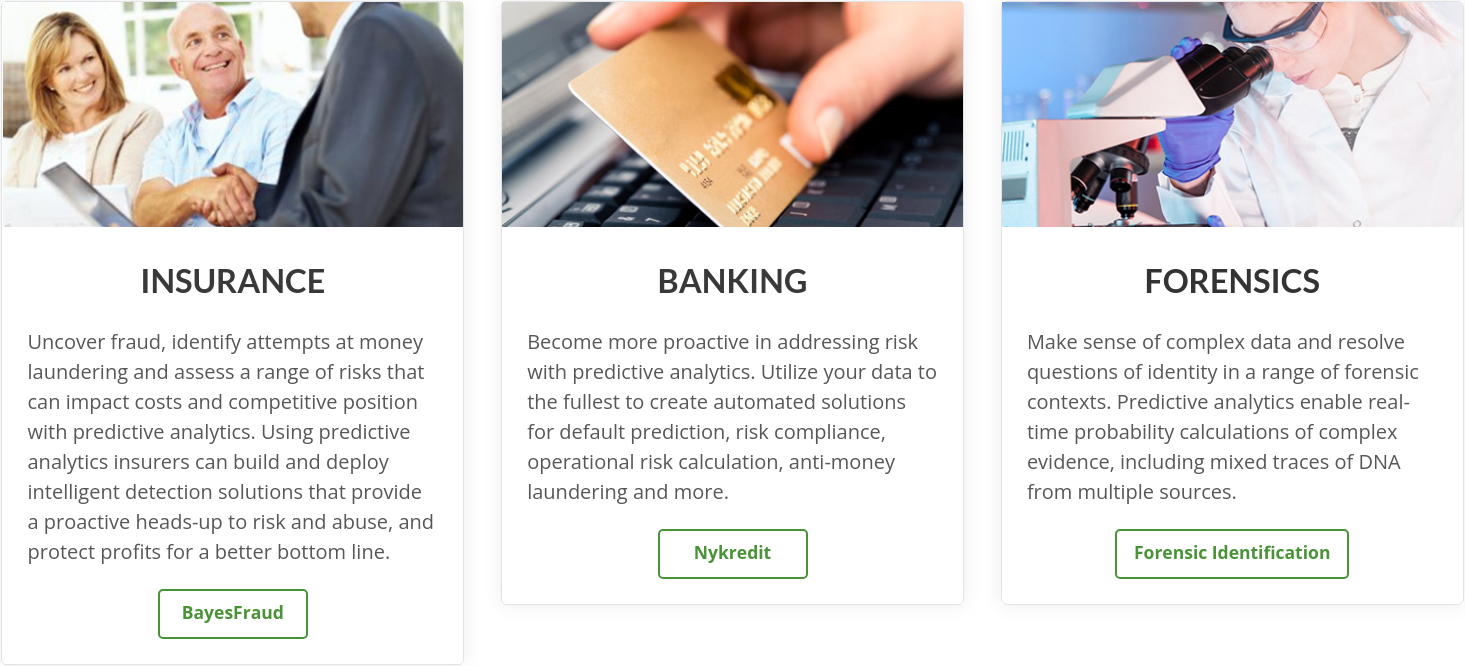
\includegraphics[width=215pt]{figures/hugin-expert/industry-applications-1.png}
  \end{textblock*}
  \begin{textblock*}{10pt}(120pt,150pt)
    
\includegraphics[width=215pt]{figures/hugin-expert/industry-applications-2.png}
  \end{textblock*}
  \only<2>{
    \begin{textblock*}{60pt}(30pt,160pt)
      \scriptsize
      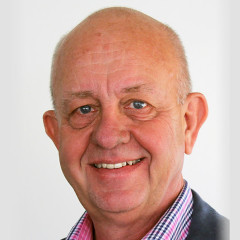
\includegraphics[width=60pt]{figures/hugin-expert/lauritzen.png}
      \textbf{ Steffen Lauritzen}\\Chairman
    \end{textblock*}
  }
\end{frame}

%------------------------------------------------------------------------------
\begin{frame}{Overview of the Junction Tree Algorithm}
  \begin{figure}
    \vspace{0.6cm} % manually adjust vertical positioning
    \scalebox{0.7}{\pptc{}{}}
  \end{figure}
  \only<2->{
    \begin{textblock*}{1pt}(280pt,45pt)
      \scalebox{0.35}{\tikzset {
  myarrow/.style= {-{Stealth[scale=1.0]}},
}

\begin{tikzpicture}[]

  % The various elements are conveniently placed using a matrix:
  \matrix[row sep=0.05cm,column sep=0.5cm] {
    % First line
                                                        &
                                                        &
    \node (d) [var, minimum size=0.7cm, fill=D] {$D$};  &
                                                       \\
    % Second line
                                                        &
    \node (b) [var, minimum size=0.7cm, fill=B] {$B$};  &
                                                        &
                                                       \\
    % Third line
    \node (a) [var, minimum size=0.7cm, fill=A] {$A$};  &
                                                        &
                                                        &
    \node (f) [var, minimum size=0.7cm, fill=F] {$F$}; \\
    % Forth line
                                                        &
    \node (c) [var, minimum size=0.7cm, fill=C] {$C$};  &
    \node (e) [var, minimum size=0.7cm, fill=E] {$E$};  &
                                                       \\
  };

  \draw [myarrow] (a) edge (b);
  \draw [myarrow] (a) edge (c);
  \draw [myarrow] (b) edge (d);
  \draw [myarrow] (b) edge (f);
  \draw [myarrow] (c) edge (e);
  \draw [myarrow] (e) edge (f);

\end{tikzpicture}

}
    \end{textblock*}
  }
  \only<3->{
    \begin{textblock*}{1pt}(280pt,95pt)
      \scalebox{0.2}{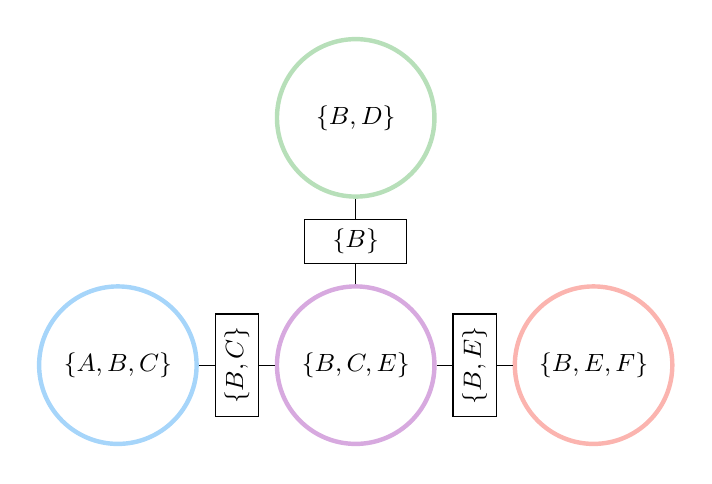
\begin{tikzpicture}[>=latex]

  \tikzset{CliqueStyle/.style =  {opacity=.4,color=#1,}}
  
  % The various elements are conveniently placed using a matrix:
  \matrix[row sep=0.26cm,column sep=0.20cm] {
    % First line
                                                         &
                                                         &
    \node (bd) [bag, minimum size=2.0cm, draw=D] {$\{B,D\}$};  &
                                                         &
                                                        \\
    % Second line
                                                         &
                                                         &
    \node (b) [hsepset] {$\{B\}$};                    &
                                                         &
                                                        \\
    % Third line
    \node (abc) [bag,minimum size=2.0cm,draw=C] {$\{A,B,C\}$};  &
    \node (bc) [vsepset] {$\{B,C\}$};                    &
    \node (bce) [bag,minimum size=2.0cm,draw=E] {$\{B,C,E\}$};  &
    \node (be) [vsepset] {$\{B,E\}$};                    &
    \node (bef) [bag,minimum size=2.0cm,draw=F] {$\{B,E,F\}$};
                                                        \\
  };

  % The diagram elements are now connected through lines:
  \path[-]
    (bd) edge (b)
    (b) edge (bce)
    (abc) edge (bc)
    (bc) edge (bce)
    (bce) edge (be)
    (be) edge (bef)
    ;

  %% Draw colored circles inside clusters corresponding to the assigned cliques
  %\node at (bd) [draw,yshift=-4.0mm] [bag,CliqueStyle=MaterialGreen] {} ;
  %\node at (abc) [draw,yshift= 5.0mm] [bag,CliqueStyle=MaterialOrange] {} ;
  %\node at (abc) [draw,yshift=-4.0mm,xshift= 3.0mm] [bag,CliqueStyle=MaterialBlue] {} ;
  %\node at (abc) [draw,yshift=-4.0mm,xshift=-3.0mm] [bag,CliqueStyle=MaterialCyan] {} ;
  %\node at (bce) [draw,yshift=-4.0mm] [bag,CliqueStyle=MaterialPurple] {} ;
  %\node at (bef) [draw,yshift=-4.0mm] [bag,CliqueStyle=MaterialRed] {} ;

\end{tikzpicture}

}
    \end{textblock*}
  }
  \only<4->{
    \begin{textblock*}{1pt}(280pt,139pt)
      \scalebox{0.2}{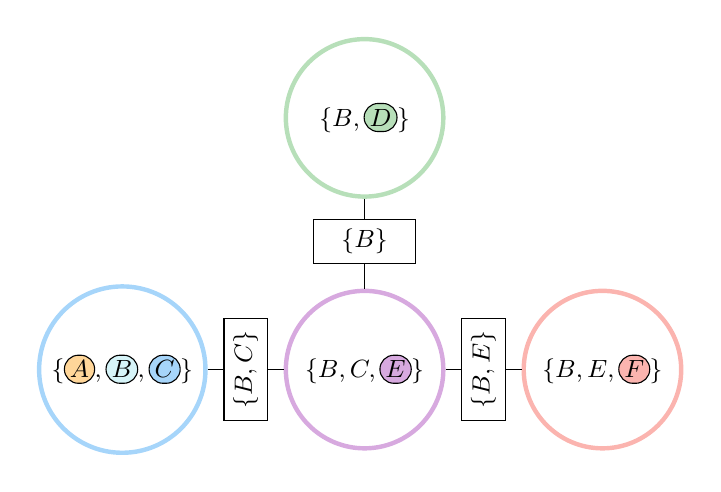
\begin{tikzpicture}[>=latex]

  \tikzset{CliqueStyle/.style =  {opacity=.4,color=#1,}}
  
  % The various elements are conveniently placed using a matrix:
  \matrix[row sep=0.26cm,column sep=0.20cm] {
    % First line
                                                         &
                                                         &
    \node (bd) [bag, minimum size=2.0cm, draw=D] {$\{B,\Circled[fill color=D]{D}\}$};  &
                                                         &
                                                        \\
    % Second line
                                                         &
                                                         &
    \node (b) [hsepset] {$\{B\}$};                    &
                                                         &
                                                        \\
    % Third line
    \node (abc) [bag,minimum size=2.0cm,draw=C] {$\{\Circled[fill color=A]{A},\Circled[fill color=B!40]{B},\Circled[fill color=C]{C}\}$};  &
    \node (bc) [vsepset] {$\{B,C\}$};                    &
    \node (bce) [bag,minimum size=2.0cm,draw=E] {$\{B,C,\Circled[fill color=E]{E}\}$};  &
    \node (be) [vsepset] {$\{B,E\}$};                    &
    \node (bef) [bag,minimum size=2.0cm,draw=F] {$\{B,E,\Circled[fill color=F]{F}\}$};
                                                        \\
  };

  % The diagram elements are now connected through lines:
  \path[-]
    (bd) edge (b)
    (b) edge (bce)
    (abc) edge (bc)
    (bc) edge (bce)
    (bce) edge (be)
    (be) edge (bef)
    ;

  %% Draw colored circles inside clusters corresponding to the assigned cliques
  %\node at (bd) [draw,yshift=-4.0mm] [bag,CliqueStyle=MaterialGreen] {} ;
  %\node at (abc) [draw,yshift= 5.0mm] [bag,CliqueStyle=MaterialOrange] {} ;
  %\node at (abc) [draw,yshift=-4.0mm,xshift= 3.0mm] [bag,CliqueStyle=MaterialBlue] {} ;
  %\node at (abc) [draw,yshift=-4.0mm,xshift=-3.0mm] [bag,CliqueStyle=MaterialCyan] {} ;
  %\node at (bce) [draw,yshift=-4.0mm] [bag,CliqueStyle=MaterialPurple] {} ;
  %\node at (bef) [draw,yshift=-4.0mm] [bag,CliqueStyle=MaterialRed] {} ;

\end{tikzpicture}

}
    \end{textblock*}
  }
  \only<5->{
    \begin{textblock*}{1pt}(280pt,176pt)
      \scalebox{0.2}{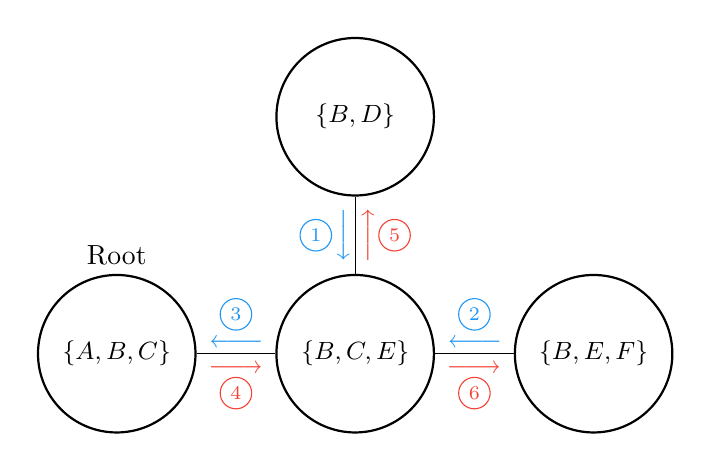
\begin{tikzpicture}[>=latex]
  
  % The various elements are conveniently placed using a matrix:
  \matrix[row sep=0.5cm,column sep=1.0cm,ampersand replacement=\&] { % column sep=1.0cm causes an Overfull \hbox warning
    % First line
                                                                                       \&
    \node (bd) [bag, thick, minimum size=2.0cm] {$\{B,D\}$};                           \&
                                                                                      \\
    % Second line
    \node (abc) [bag, thick, minimum size=2.0cm, label={above:{Root}}] {$\{A,B,C\}$};  \&
    \node (bce) [bag, thick, minimum size=2.0cm] {$\{B,C,E\}$};                        \&
    \node (bef) [bag, thick, minimum size=2.0cm] {$\{B,E,F\}$};                       \\
  };
    
  % The diagram elements are now connected through lines:
  \path[-]
    (bd) edge (bce)
    (abc) edge (bce)
    (bce) edge (bef)
    ;

  \msgcircle{left}{down}{bd}{bce}{0.5}{$1$}{MaterialBlue};
  \msgcircle{up}{left}{bef}{bce}{0.5}{$2$}{MaterialBlue};
  \msgcircle{up}{left}{bce}{abc}{0.5}{$3$}{MaterialBlue};
  \msgcircle{down}{right}{abc}{bce}{0.5}{$4$}{MaterialRed};
  \msgcircle{right}{up}{bce}{bd}{0.5}{$5$}{MaterialRed};
  \msgcircle{down}{right}{bce}{bef}{0.5}{$6$}{MaterialRed};
    
\end{tikzpicture}

}
    \end{textblock*}
  }
\end{frame}

%==============================================================================
\subsection{Probabilistic Graphical Model}
%==============================================================================

%------------------------------------------------------------------------------
\begin{frame}{Overview}
  \begin{figure}
    \vspace{0.6cm} % manually adjust vertical positioning
    \scalebox{0.7}{\pptc{Probabilistic Graphical Model}{}}
  \end{figure}
\end{frame}

%------------------------------------------------------------------------------
\begin{frame}{Probabilistic Graphical Model}

  \begin{columns}

    % Column 1
    \begin{column}{0.6\textwidth}

      \begin{block}{Joint probability distribution}
        \begin{align*}
        &P(\mathcal{V}) = \prod_{V\in\mathcal{V}} P(V \mid pa(V))&
        \end{align*}
      \end{block}
      \begin{block}{Conditional probability distribution}
        \begin{table}
          $P(\textcolor{MaterialCyan}{B} \mid A)$ = 
          \begin{tabular}{ c|c c } 
            & \multicolumn{2}{|c}{$P(b \mid a)$} \\
            $a$ & yes & no \\ 
            \hline
            yes & 0.1 & 0.5 \\ 
            no & 0.4 & 0.3 \\ 
          \end{tabular}
          \hfill
        \end{table}
      \end{block}

      %\begin{block}{Joint probability distribution}
      %  \begin{align*}
      %    &P(\mathcal{V}) = \prod_{V\in\mathcal{V}} P(V \mid pa(V))&
      %  \end{align*}
      %\end{block}

    \end{column}

    % Column 2    
    \begin{column}{0.4\textwidth}

      \begin{figure}
        \scalebox{0.8}{\tikzset {
  myarrow/.style= {-{Stealth[scale=1.0]}},
}

\begin{tikzpicture}[]

  % The various elements are conveniently placed using a matrix:
  \matrix[row sep=0.05cm,column sep=0.5cm] {
    % First line
                                                        &
                                                        &
    \node (d) [var, minimum size=0.7cm, fill=D] {$D$};  &
                                                       \\
    % Second line
                                                        &
    \node (b) [var, minimum size=0.7cm, fill=B] {$B$};  &
                                                        &
                                                       \\
    % Third line
    \node (a) [var, minimum size=0.7cm, fill=A] {$A$};  &
                                                        &
                                                        &
    \node (f) [var, minimum size=0.7cm, fill=F] {$F$}; \\
    % Forth line
                                                        &
    \node (c) [var, minimum size=0.7cm, fill=C] {$C$};  &
    \node (e) [var, minimum size=0.7cm, fill=E] {$E$};  &
                                                       \\
  };

  \draw [myarrow] (a) edge (b);
  \draw [myarrow] (a) edge (c);
  \draw [myarrow] (b) edge (d);
  \draw [myarrow] (b) edge (f);
  \draw [myarrow] (c) edge (e);
  \draw [myarrow] (e) edge (f);

\end{tikzpicture}

}
        \caption{A Bayesian network\footnotemark}
      \end{figure}

    \end{column}

  \end{columns}
  \footnotetext{Example borrowed from Mark A. Paskin - A Short Course on Graphical Models}
\end{frame}

%------------------------------------------------------------------------------
\begin{frame}{Starting Point}
  \begin{figure}
    \scalebox{1.0}{\tikzset {
  myarrow/.style= {-{Stealth[scale=1.0]}},
}

\begin{tikzpicture}[]

  % The various elements are conveniently placed using a matrix:
  \matrix[row sep=0.05cm,column sep=0.5cm] {
    % First line
                                                        &
                                                        &
    \node (d) [var, minimum size=0.7cm, fill=D] {$D$};  &
                                                       \\
    % Second line
                                                        &
    \node (b) [var, minimum size=0.7cm, fill=B] {$B$};  &
                                                        &
                                                       \\
    % Third line
    \node (a) [var, minimum size=0.7cm, fill=A] {$A$};  &
                                                        &
                                                        &
    \node (f) [var, minimum size=0.7cm, fill=F] {$F$}; \\
    % Forth line
                                                        &
    \node (c) [var, minimum size=0.7cm, fill=C] {$C$};  &
    \node (e) [var, minimum size=0.7cm, fill=E] {$E$};  &
                                                       \\
  };

  \draw [myarrow] (a) edge (b);
  \draw [myarrow] (a) edge (c);
  \draw [myarrow] (b) edge (d);
  \draw [myarrow] (b) edge (f);
  \draw [myarrow] (c) edge (e);
  \draw [myarrow] (e) edge (f);

\end{tikzpicture}

}
    \caption{A Bayesian network}
  \end{figure}
\end{frame}

%==============================================================================
\subsection{Moralization}
%==============================================================================

%------------------------------------------------------------------------------
\begin{frame}{Overview}
  \begin{figure}
    \vspace{0.6cm} % manually adjust vertical positioning
    \scalebox{0.7}{\pptc{Probabilistic Graphical Model}{Moralization}}
  \end{figure}
\end{frame}

%------------------------------------------------------------------------------
\begin{frame}{Moralization}
  \centering
  {\footnotesize Marry the parents of each variable and drop the directions of the edges.}
  \begin{figure}[h]  
    \begin{subfigure}[b]{0.49\linewidth}
      \centering
      \scalebox{1.0}{\tikzset {
  myarrow/.style= {-{Stealth[scale=1.0]}},
}

\begin{tikzpicture}[]

  % The various elements are conveniently placed using a matrix:
  \matrix[row sep=0.05cm,column sep=0.5cm] {
    % First line
                                                        &
                                                        &
    \node (d) [var, minimum size=0.7cm, fill=D] {$D$};  &
                                                       \\
    % Second line
                                                        &
    \node (b) [var, minimum size=0.7cm, fill=B] {$B$};  &
                                                        &
                                                       \\
    % Third line
    \node (a) [var, minimum size=0.7cm, fill=A] {$A$};  &
                                                        &
                                                        &
    \node (f) [var, minimum size=0.7cm, fill=F] {$F$}; \\
    % Forth line
                                                        &
    \node (c) [var, minimum size=0.7cm, fill=C] {$C$};  &
    \node (e) [var, minimum size=0.7cm, fill=E] {$E$};  &
                                                       \\
  };

  \draw [myarrow] (a) edge (b);
  \draw [myarrow] (a) edge (c);
  \draw [myarrow] (b) edge (d);
  \draw [myarrow] (b) edge (f);
  \draw [myarrow] (c) edge (e);
  \draw [myarrow] (e) edge (f);

\end{tikzpicture}

}
      %\resizebox{\textwidth}{!}{\tikzset {
  myarrow/.style= {-{Stealth[scale=1.0]}},
}

\begin{tikzpicture}[]

  % The various elements are conveniently placed using a matrix:
  \matrix[row sep=0.05cm,column sep=0.5cm] {
    % First line
                                                        &
                                                        &
    \node (d) [var, minimum size=0.7cm, fill=D] {$D$};  &
                                                       \\
    % Second line
                                                        &
    \node (b) [var, minimum size=0.7cm, fill=B] {$B$};  &
                                                        &
                                                       \\
    % Third line
    \node (a) [var, minimum size=0.7cm, fill=A] {$A$};  &
                                                        &
                                                        &
    \node (f) [var, minimum size=0.7cm, fill=F] {$F$}; \\
    % Forth line
                                                        &
    \node (c) [var, minimum size=0.7cm, fill=C] {$C$};  &
    \node (e) [var, minimum size=0.7cm, fill=E] {$E$};  &
                                                       \\
  };

  \draw [myarrow] (a) edge (b);
  \draw [myarrow] (a) edge (c);
  \draw [myarrow] (b) edge (d);
  \draw [myarrow] (b) edge (f);
  \draw [myarrow] (c) edge (e);
  \draw [myarrow] (e) edge (f);

\end{tikzpicture}

}
      \caption{Bayesian network}
    \end{subfigure}
    \begin{subfigure}[b]{0.49\linewidth}
      \centering
      \scalebox{1.0}{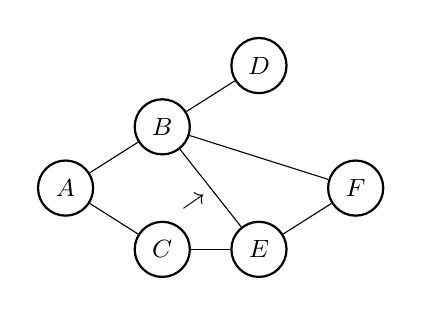
\begin{tikzpicture}[]

  \tikzset{CliqueStyle/.style =  {opacity=.4,line width=14 mm,line cap=round,color=#1,join=round}}
  
  % The various elements are conveniently placed using a matrix:
  \matrix[row sep=0.05cm,column sep=0.5cm] {
    % First line
                                                  &
                                                  &
    \node (d)   [var, minimum size=0.7cm] {$D$};  &
                                                 \\
    % Second line
                                                  &
    \node (b)   [var, minimum size=0.7cm] {$B$};  &
                                                  &
                                                 \\
    % Third line
    \node (a) [var, minimum size=0.7cm] {$A$};    &
                                                  &
                                                  &
    \node (f) [var, minimum size=0.7cm] {$F$};   \\
    % Forth line
                                                  &
    \node (c)   [var, minimum size=0.7cm] {$C$};  &
    \node (e)   [var, minimum size=0.7cm] {$E$};  &
                                                 \\
  };

  \draw (a) edge (b);
  \draw (a) edge (c);
  \draw (b) edge (d);
  \draw (b) edge (f);
  \draw [] (b) edge (e); % add annotation saying that this is the added edge
  \draw (c) edge (e);
  \draw (e) edge (f);

  \path (b) -- node[anchor=center,xshift=-0.2cm,yshift=-0.2cm,rotate=35] (be) {$\rightarrow$} (e);

  %\begin{pgfonlayer}{background}
  %  \draw [CliqueStyle=MaterialBlue] (a.center) -- (b.center) ;
  %  \draw [CliqueStyle=MaterialGreen] (b.center) -- (d.center) ;
  %  \draw [CliqueStyle=MaterialYellow] (a.center) -- (c.center) ;
  %  \draw [CliqueStyle=MaterialRed] (c.center) -- (e.center) ;
  %  \draw [CliqueStyle=MaterialCyan] (b.center) -- (f.center) -- (e.center) -- (b.center);
  %\end{pgfonlayer}

\end{tikzpicture}

}
      %\resizebox{\textwidth}{!}{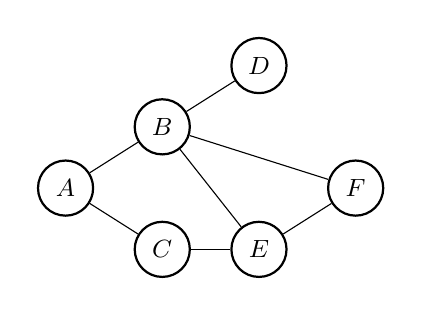
\begin{tikzpicture}[]

  \tikzset{CliqueStyle/.style =  {opacity=.4,line width=14 mm,line cap=round,color=#1,join=round}}
  
  % The various elements are conveniently placed using a matrix:
  \matrix[row sep=0.05cm,column sep=0.5cm] {
    % First line
                                                  &
                                                  &
    \node (d)   [var, minimum size=0.7cm] {$D$};  &
                                                 \\
    % Second line
                                                  &
    \node (b)   [var, minimum size=0.7cm] {$B$};  &
                                                  &
                                                 \\
    % Third line
    \node (a) [var, minimum size=0.7cm] {$A$};    &
                                                  &
                                                  &
    \node (f) [var, minimum size=0.7cm] {$F$};   \\
    % Forth line
                                                  &
    \node (c)   [var, minimum size=0.7cm] {$C$};  &
    \node (e)   [var, minimum size=0.7cm] {$E$};  &
                                                 \\
  };

  \draw (a) edge (b);
  \draw (a) edge (c);
  \draw (b) edge (d);
  \draw (b) edge (f);
  \draw [] (b) edge (e); % add annotation saying that this is the added edge
  \draw (c) edge (e);
  \draw (e) edge (f);

  %\path (b) -- node[anchor=center,xshift=-0.2cm,yshift=-0.2cm,rotate=35] (be) {$\rightarrow$} (e);

  %\begin{pgfonlayer}{background}
  %  \draw [CliqueStyle=MaterialBlue] (a.center) -- (b.center) ;
  %  \draw [CliqueStyle=MaterialGreen] (b.center) -- (d.center) ;
  %  \draw [CliqueStyle=MaterialYellow] (a.center) -- (c.center) ;
  %  \draw [CliqueStyle=MaterialRed] (c.center) -- (e.center) ;
  %  \draw [CliqueStyle=MaterialCyan] (b.center) -- (f.center) -- (e.center) -- (b.center);
  %\end{pgfonlayer}

\end{tikzpicture}

}
      \caption{Moral graph}
    \end{subfigure}
    \caption{Moralization}
  \end{figure}  
\end{frame}

%------------------------------------------------------------------------------
\begin{frame}{Moralization}
  \begin{figure}
    \scalebox{1.0}{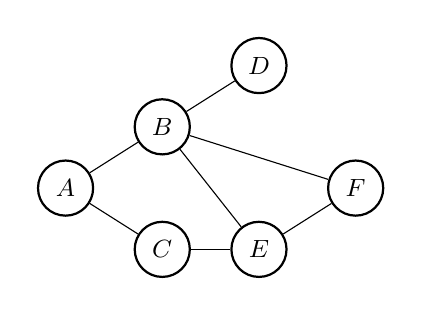
\begin{tikzpicture}[]

  \tikzset{CliqueStyle/.style =  {opacity=.4,line width=14 mm,line cap=round,color=#1,join=round}}
  
  % The various elements are conveniently placed using a matrix:
  \matrix[row sep=0.05cm,column sep=0.5cm] {
    % First line
                                                  &
                                                  &
    \node (d)   [var, minimum size=0.7cm] {$D$};  &
                                                 \\
    % Second line
                                                  &
    \node (b)   [var, minimum size=0.7cm] {$B$};  &
                                                  &
                                                 \\
    % Third line
    \node (a) [var, minimum size=0.7cm] {$A$};    &
                                                  &
                                                  &
    \node (f) [var, minimum size=0.7cm] {$F$};   \\
    % Forth line
                                                  &
    \node (c)   [var, minimum size=0.7cm] {$C$};  &
    \node (e)   [var, minimum size=0.7cm] {$E$};  &
                                                 \\
  };

  \draw (a) edge (b);
  \draw (a) edge (c);
  \draw (b) edge (d);
  \draw (b) edge (f);
  \draw [] (b) edge (e); % add annotation saying that this is the added edge
  \draw (c) edge (e);
  \draw (e) edge (f);

  %\path (b) -- node[anchor=center,xshift=-0.2cm,yshift=-0.2cm,rotate=35] (be) {$\rightarrow$} (e);

  %\begin{pgfonlayer}{background}
  %  \draw [CliqueStyle=MaterialBlue] (a.center) -- (b.center) ;
  %  \draw [CliqueStyle=MaterialGreen] (b.center) -- (d.center) ;
  %  \draw [CliqueStyle=MaterialYellow] (a.center) -- (c.center) ;
  %  \draw [CliqueStyle=MaterialRed] (c.center) -- (e.center) ;
  %  \draw [CliqueStyle=MaterialCyan] (b.center) -- (f.center) -- (e.center) -- (b.center);
  %\end{pgfonlayer}

\end{tikzpicture}

}
    \caption{Moral Graph}
  \end{figure}
\end{frame}

%==============================================================================
\subsection{Triangulation}
%==============================================================================

%------------------------------------------------------------------------------
\begin{frame}{Overview}
  \begin{figure}
    \vspace{0.6cm} % manually adjust vertical positioning
    \scalebox{0.7}{\pptc{Probabilistic Graphical Model}{Triangulation}}
  \end{figure}
\end{frame}

%------------------------------------------------------------------------------
\begin{frame}{Triangulation}
  \centering
  {\footnotesize
    \only<1>{
      Consists of removing every cycle of length greater than three in a graph.
    }
    \only<2>{
      We do so by connecting two nonadjacent nodes in every cycle of length $>$ three.
    }
    \only<3-4>{
      An optimal triangulation minimizes the sum of the state space sizes of the cliques.
    }
    \only<4>{
      This is equivalent to minimizing the size of the largest clique.
    }
    \only<5>{
      This problem is \textit{NP-complete}.
    }
  }

  \begin{figure}[h]  
    \begin{subfigure}[b]{0.49\linewidth}
      \centering
      \scalebox{1.0}{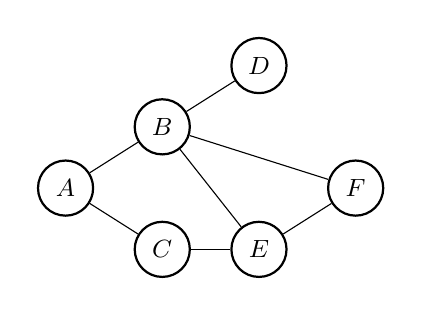
\begin{tikzpicture}[]

  \tikzset{CliqueStyle/.style =  {opacity=.4,line width=14 mm,line cap=round,color=#1,join=round}}
  
  % The various elements are conveniently placed using a matrix:
  \matrix[row sep=0.05cm,column sep=0.5cm] {
    % First line
                                                  &
                                                  &
    \node (d)   [var, minimum size=0.7cm] {$D$};  &
                                                 \\
    % Second line
                                                  &
    \node (b)   [var, minimum size=0.7cm] {$B$};  &
                                                  &
                                                 \\
    % Third line
    \node (a) [var, minimum size=0.7cm] {$A$};    &
                                                  &
                                                  &
    \node (f) [var, minimum size=0.7cm] {$F$};   \\
    % Forth line
                                                  &
    \node (c)   [var, minimum size=0.7cm] {$C$};  &
    \node (e)   [var, minimum size=0.7cm] {$E$};  &
                                                 \\
  };

  \draw (a) edge (b);
  \draw (a) edge (c);
  \draw (b) edge (d);
  \draw (b) edge (f);
  \draw [] (b) edge (e); % add annotation saying that this is the added edge
  \draw (c) edge (e);
  \draw (e) edge (f);

  %\path (b) -- node[anchor=center,xshift=-0.2cm,yshift=-0.2cm,rotate=35] (be) {$\rightarrow$} (e);

  %\begin{pgfonlayer}{background}
  %  \draw [CliqueStyle=MaterialBlue] (a.center) -- (b.center) ;
  %  \draw [CliqueStyle=MaterialGreen] (b.center) -- (d.center) ;
  %  \draw [CliqueStyle=MaterialYellow] (a.center) -- (c.center) ;
  %  \draw [CliqueStyle=MaterialRed] (c.center) -- (e.center) ;
  %  \draw [CliqueStyle=MaterialCyan] (b.center) -- (f.center) -- (e.center) -- (b.center);
  %\end{pgfonlayer}

\end{tikzpicture}

}
      %\resizebox{\textwidth}{!}{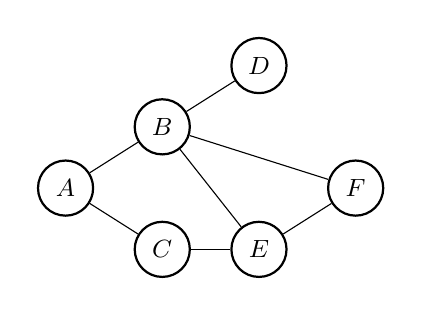
\begin{tikzpicture}[]

  \tikzset{CliqueStyle/.style =  {opacity=.4,line width=14 mm,line cap=round,color=#1,join=round}}
  
  % The various elements are conveniently placed using a matrix:
  \matrix[row sep=0.05cm,column sep=0.5cm] {
    % First line
                                                  &
                                                  &
    \node (d)   [var, minimum size=0.7cm] {$D$};  &
                                                 \\
    % Second line
                                                  &
    \node (b)   [var, minimum size=0.7cm] {$B$};  &
                                                  &
                                                 \\
    % Third line
    \node (a) [var, minimum size=0.7cm] {$A$};    &
                                                  &
                                                  &
    \node (f) [var, minimum size=0.7cm] {$F$};   \\
    % Forth line
                                                  &
    \node (c)   [var, minimum size=0.7cm] {$C$};  &
    \node (e)   [var, minimum size=0.7cm] {$E$};  &
                                                 \\
  };

  \draw (a) edge (b);
  \draw (a) edge (c);
  \draw (b) edge (d);
  \draw (b) edge (f);
  \draw [] (b) edge (e); % add annotation saying that this is the added edge
  \draw (c) edge (e);
  \draw (e) edge (f);

  %\path (b) -- node[anchor=center,xshift=-0.2cm,yshift=-0.2cm,rotate=35] (be) {$\rightarrow$} (e);

  %\begin{pgfonlayer}{background}
  %  \draw [CliqueStyle=MaterialBlue] (a.center) -- (b.center) ;
  %  \draw [CliqueStyle=MaterialGreen] (b.center) -- (d.center) ;
  %  \draw [CliqueStyle=MaterialYellow] (a.center) -- (c.center) ;
  %  \draw [CliqueStyle=MaterialRed] (c.center) -- (e.center) ;
  %  \draw [CliqueStyle=MaterialCyan] (b.center) -- (f.center) -- (e.center) -- (b.center);
  %\end{pgfonlayer}

\end{tikzpicture}

}
      \caption{Moral graph}
    \end{subfigure}
    \begin{subfigure}[b]{0.49\linewidth}
      \centering
      \scalebox{1.0}{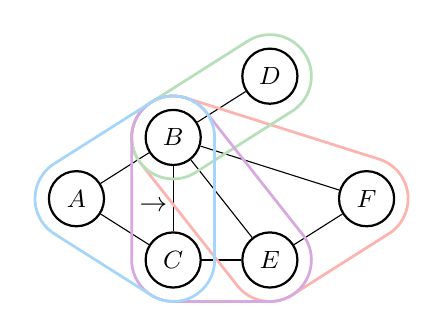
\begin{tikzpicture}[
  %every node/.style={black},
  %every path/.style={red},
  transform shape]

  % The various elements are conveniently placed using a matrix:
  \matrix[row sep=0.05cm,column sep=0.5cm] {
    % First line
                                                  &
                                                  &
    \node (d)   [var, minimum size=0.7cm] {$D$};  &
                                                 \\
    % Second line
                                                  &
    \node (b)   [var, minimum size=0.7cm] {$B$};  &
                                                  &
                                                 \\
    % Third line
    \node (a) [var, minimum size=0.7cm] {$A$};    &
                                                  &
                                                  &
    \node (f) [var, minimum size=0.7cm] {$F$};   \\
    % Forth line
                                                  &
    \node (c)   [var, minimum size=0.7cm] {$C$};  &
    \node (e)   [var, minimum size=0.7cm] {$E$};  &
                                                 \\
  };

  \draw (a) edge (b);
  \draw (a) edge (c);
  \draw [](b) edge (c);
  \draw (b) edge (d);
  \draw (b) edge (f);
  \draw (b) edge (e);
  \draw (c) edge (e);
  \draw (e) edge (f);

  \path (b) -- node[anchor=center,xshift=-0.25cm,yshift=-0.1cm] (bc) {$\rightarrow$} (c);

  \draw[F,line width=1pt] \convexpath{b,f,e}{15pt};
  \draw[D,line width=1pt] \convexpath{b,d}{15pt};
  \draw[E,line width=1pt] \convexpath{b,e,c}{15pt};
  \draw[C,line width=1pt] \convexpath{a,b,c}{15pt};

\end{tikzpicture}

}
      %\resizebox{\textwidth}{!}{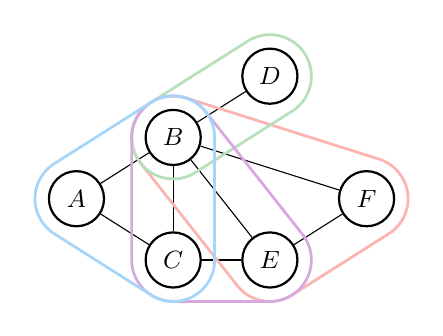
\begin{tikzpicture}[
  %every node/.style={black},
  %every path/.style={red},
  transform shape]

  % The various elements are conveniently placed using a matrix:
  \matrix[row sep=0.05cm,column sep=0.5cm] {
    % First line
                                                  &
                                                  &
    \node (d)   [var, minimum size=0.7cm] {$D$};  &
                                                 \\
    % Second line
                                                  &
    \node (b)   [var, minimum size=0.7cm] {$B$};  &
                                                  &
                                                 \\
    % Third line
    \node (a) [var, minimum size=0.7cm] {$A$};    &
                                                  &
                                                  &
    \node (f) [var, minimum size=0.7cm] {$F$};   \\
    % Forth line
                                                  &
    \node (c)   [var, minimum size=0.7cm] {$C$};  &
    \node (e)   [var, minimum size=0.7cm] {$E$};  &
                                                 \\
  };

  \draw (a) edge (b);
  \draw (a) edge (c);
  \draw [](b) edge (c);
  \draw (b) edge (d);
  \draw (b) edge (f);
  \draw (b) edge (e);
  \draw (c) edge (e);
  \draw (e) edge (f);

  %\path (b) -- node[anchor=center,xshift=-0.25cm,yshift=-0.1cm] (bc) {$\rightarrow$} (c);

  \draw[F,line width=1pt] \convexpath{b,f,e}{15pt};
  \draw[D,line width=1pt] \convexpath{b,d}{15pt};
  \draw[E,line width=1pt] \convexpath{b,e,c}{15pt};
  \draw[C,line width=1pt] \convexpath{a,b,c}{15pt};

\end{tikzpicture}

}
      \caption{Triangulated graph}
    \end{subfigure}
    \caption{Triangulation}
  \end{figure}
\end{frame}
\note{
  - This is the hardest of all steps. And when I say hard, I mean it literally.
  This problem is NP-hard.
  - The goal is to get rid of all cycles of length greater than 3!
  - Note that a byproduct of triangulation is the set of maximal cliques of the
  triangulated graph, which are extremely useful for the junction algorithm:
  these maximal cliques become the nodes of the final junction tree.
  - The overall goal is to minimize the state space size of the system.
  - This is equivalent to minimizing the number of vars in the largest
  clique/cluster.
  - The enclosed sets of nodes are maximal cliques which, in this case, become
  the clusters of the junction tree.
  - A clique is a set of variables in which all variables are connected to each
  other.
  - A maximal clique is a one that is not contained in a larger one.
}

%------------------------------------------------------------------------------
%------------------------------------------------------------------------------
%%
%------------------------------------------------------------------------------

\begin{frame}[fragile]{Triangulation: Min-fill Algorithm}

\centering

{\footnotesize
  We will now demonstrate the \textbf{min-fill algorithm} \cite{Kjærulff90triangulationof}:
  A greedy, polynomial-time \textit{heuristic} that produces high-quality
  triangulations in real-world settings.
}

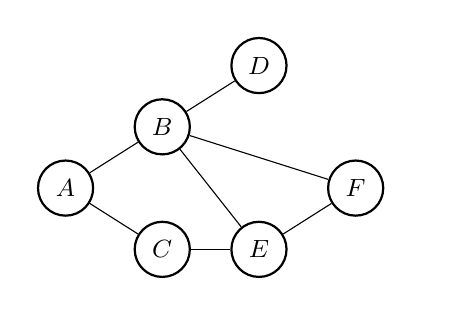
\begin{tikzpicture}[transform shape]

  \matrix[row sep=0.05cm,column sep=0.5cm] {
    % First line
                                                   &
                                                   &
    \node (d1)   [var, minimum size=0.7cm] {$D$};  &
                                                   &
                                                  \\
    % Second line
                                                   &
    \node (b1)   [var, minimum size=0.7cm] {$B$};  &
                                                   &
                                                   &
                                                  \\
    % Third line
    \node (a1) [var, minimum size=0.7cm] {$A$};    &
                                                   &
                                                   &
    \node (f1) [var, minimum size=0.7cm] {$F$};    &
                                                  \\
    % Forth line
                                                   &
    \node (c1)   [var, minimum size=0.7cm] {$C$};  &
    \node (e1)   [var, minimum size=0.7cm] {$E$};  &
                                                   &
                                                  \\
  };

  \draw (a1) edge (b1);
  \draw (a1) edge (c1);
  %\draw (b1) edge (c1);
  \draw (b1) edge (d1);
  \draw (b1) edge (f1);
  \draw (b1) edge (e1);
  \draw (c1) edge (e1);
  \draw (e1) edge (f1);

  %\draw[F,line width=1pt] \convexpath{b1,f1,e1}{15pt};
  %\draw[D,line width=1pt] \convexpath{b1,d1}{15pt};
  %\draw[E,line width=1pt] \convexpath{b1,e1,c1}{15pt};
  %\draw[C,line width=1pt] \convexpath{a1,b1,c1}{15pt};

\end{tikzpicture}

\end{frame}

%------------------------------------------------------------------------------
%%
%------------------------------------------------------------------------------

\begin{frame}[fragile]{Triangulation: Min-fill Algorithm}

\centering

{\footnotesize Subscripts denote the variable's \textit{cardinality}.}

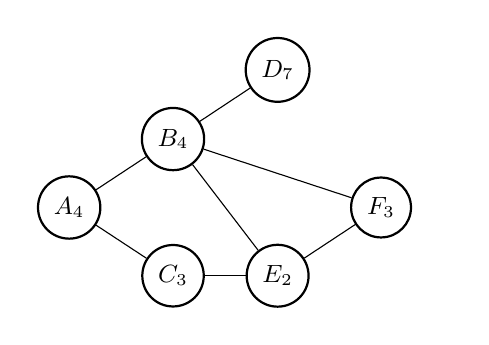
\begin{tikzpicture}[transform shape]

  \matrix[row sep=0.05cm,column sep=0.5cm] {
    % First line
                                                     &
                                                     &
    \node (d1)   [var, minimum size=0.7cm] {$D_7$};  &
                                                     &
                                                    \\
    % Second line
                                                     &
    \node (b1)   [var, minimum size=0.7cm] {$B_4$};  &
                                                     &
                                                     &
                                                    \\
    % Third line
    \node (a1) [var, minimum size=0.7cm] {$A_4$};    &
                                                     &
                                                     &
    \node (f1) [var, minimum size=0.7cm] {$F_3$};    &
                                                    \\
    % Forth line
                                                     &
    \node (c1)   [var, minimum size=0.7cm] {$C_3$};  &
    \node (e1)   [var, minimum size=0.7cm] {$E_2$};  &
                                                     &
                                                    \\
  };

  \draw (a1) edge (b1);
  \draw (a1) edge (c1);
  %\draw (b1) edge (c1);
  \draw (b1) edge (d1);
  \draw (b1) edge (f1);
  \draw (b1) edge (e1);
  \draw (c1) edge (e1);
  \draw (e1) edge (f1);

  %\draw[F,line width=1pt] \convexpath{b1,f1,e1}{15pt};
  %\draw[D,line width=1pt] \convexpath{b1,d1}{15pt};
  %\draw[E,line width=1pt] \convexpath{b1,e1,c1}{15pt};
  %\draw[C,line width=1pt] \convexpath{a1,b1,c1}{15pt};

\end{tikzpicture}

\end{frame}

%------------------------------------------------------------------------------
%%
%------------------------------------------------------------------------------

\begin{frame}[fragile]{Triangulation: Min-fill Algorithm}

\centering

{\footnotesize Make a copy of the graph.}

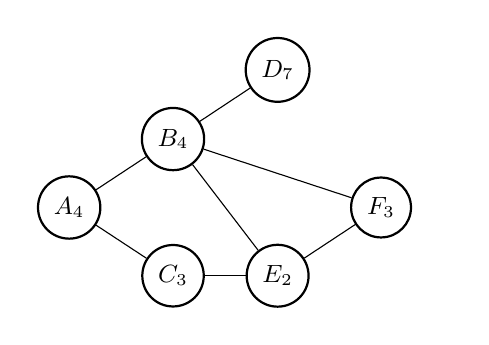
\begin{tikzpicture}[transform shape]

  \matrix[row sep=0.05cm,column sep=0.5cm] {
    % First line
                                                     &
                                                     &
    \node (d1)   [var, minimum size=0.7cm] {$D_7$};  &
                                                     &
                                                    \\
    % Second line
                                                     &
    \node (b1)   [var, minimum size=0.7cm] {$B_4$};  &
                                                     &
                                                     &
                                                    \\
    % Third line
    \node (a1) [var, minimum size=0.7cm] {$A_4$};    &
                                                     &
                                                     &
    \node (f1) [var, minimum size=0.7cm] {$F_3$};    &
                                                    \\
    % Forth line
                                                     &
    \node (c1)   [var, minimum size=0.7cm] {$C_3$};  &
    \node (e1)   [var, minimum size=0.7cm] {$E_2$};  &
                                                     &
                                                    \\
  };

  \draw (a1) edge (b1);
  \draw (a1) edge (c1);
  %\draw (b1) edge (c1);
  \draw (b1) edge (d1);
  \draw (b1) edge (f1);
  \draw (b1) edge (e1);
  \draw (c1) edge (e1);
  \draw (e1) edge (f1);

  %\draw[F,line width=1pt] \convexpath{b1,f1,e1}{15pt};
  %\draw[D,line width=1pt] \convexpath{b1,d1}{15pt};
  %\draw[E,line width=1pt] \convexpath{b1,e1,c1}{15pt};
  %\draw[C,line width=1pt] \convexpath{a1,b1,c1}{15pt};

\end{tikzpicture}
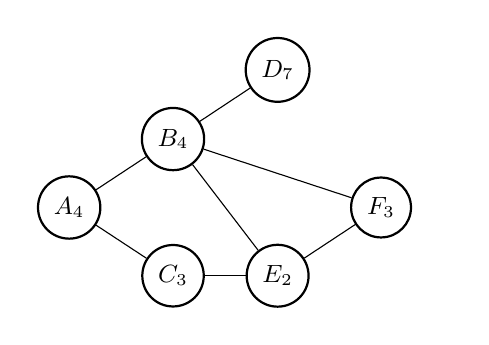
\begin{tikzpicture}[transform shape]
  \matrix[row sep=0.05cm,column sep=0.5cm] {
    % First line
                                                     &
                                                     &
    \node (d2)   [var, minimum size=0.7cm] {$D_7$};  &
                                                     &
                                                    \\
    % Second line
                                                     &
    \node (b2)   [var, minimum size=0.7cm] {$B_4$};  &
                                                     &
                                                     &
                                                    \\
    % Third line
    \node (a2) [var, minimum size=0.7cm] {$A_4$};    &
                                                     &
                                                     &
    \node (f2) [var, minimum size=0.7cm] {$F_3$};    &
                                                    \\
    % Forth line
                                                     &
    \node (c2)   [var, minimum size=0.7cm] {$C_3$};  &
    \node (e2)   [var, minimum size=0.7cm] {$E_2$};  &
                                                     &
                                                    \\
  };

  \draw (a2) edge (b2);
  \draw (a2) edge (c2);
  %\draw (b2) edge (c2);
  \draw (b2) edge (d2);
  \draw (b2) edge (f2);
  \draw (b2) edge (e2);
  \draw (c2) edge (e2);
  \draw (e2) edge (f2);

  %\path (b1) -- node[anchor=center,xshift=-0.25cm,yshift=-0.1cm] (bc) {$\rightarrow$} (c1);

  %\draw[F,line width=1pt] \convexpath{b2,f2,e2}{15pt};
  %\draw[D,line width=1pt] \convexpath{b2,d2}{15pt};
  %\draw[E,line width=1pt] \convexpath{b2,e2,c2}{15pt};
  %\draw[C,line width=1pt] \convexpath{a2,b2,c2}{15pt};

\end{tikzpicture}

\end{frame}

%------------------------------------------------------------------------------
%%
%------------------------------------------------------------------------------

\begin{frame}[fragile]{Triangulation: Min-fill Algorithm}

\centering

{\footnotesize Select a node in the left graph according to the criterion described below.}

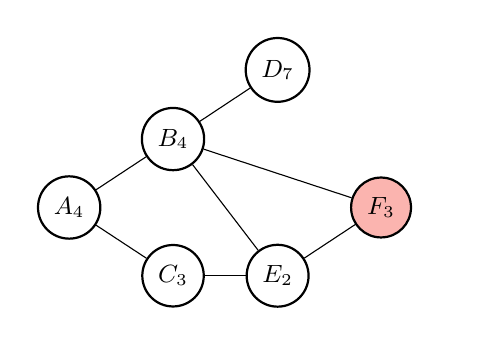
\begin{tikzpicture}[transform shape]

  \matrix[row sep=0.05cm,column sep=0.5cm] {
    % First line
                                                           &
                                                           &
    \node (d1)   [var, minimum size=0.7cm] {$D_7$};        &
                                                           &
                                                          \\
    % Second line
                                                           &
    \node (b1)   [var, minimum size=0.7cm] {$B_4$};        &
                                                           &
                                                           &
                                                          \\
    % Third line
    \node (a1) [var, minimum size=0.7cm] {$A_4$};          &
                                                           &
                                                           &
    \node (f1) [var, minimum size=0.7cm, fill=F] {$F_3$};  &
                                                          \\
    % Forth line
                                                           &
    \node (c1)   [var, minimum size=0.7cm] {$C_3$};        &
    \node (e1)   [var, minimum size=0.7cm] {$E_2$};        &
                                                           &
                                                          \\
  };

  \draw (a1) edge (b1);
  \draw (a1) edge (c1);
  %\draw (b1) edge (c1);
  \draw (b1) edge (d1);
  \draw (b1) edge (f1);
  \draw (b1) edge (e1);
  \draw (c1) edge (e1);
  \draw (e1) edge (f1);

  %\draw[F,line width=1pt] \convexpath{b1,f1,e1}{15pt};
  %\draw[D,line width=1pt] \convexpath{b1,d1}{15pt};
  %\draw[E,line width=1pt] \convexpath{b1,e1,c1}{15pt};
  %\draw[C,line width=1pt] \convexpath{a1,b1,c1}{15pt};

\end{tikzpicture}
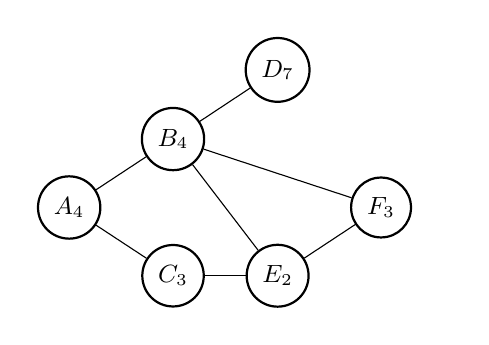
\begin{tikzpicture}[transform shape]
  \matrix[row sep=0.05cm,column sep=0.5cm] {
    % First line
                                                     &
                                                     &
    \node (d2)   [var, minimum size=0.7cm] {$D_7$};  &
                                                     &
                                                    \\
    % Second line
                                                     &
    \node (b2)   [var, minimum size=0.7cm] {$B_4$};  &
                                                     &
                                                     &
                                                    \\
    % Third line
    \node (a2) [var, minimum size=0.7cm] {$A_4$};    &
                                                     &
                                                     &
    \node (f2) [var, minimum size=0.7cm] {$F_3$};    &
                                                    \\
    % Forth line
                                                     &
    \node (c2)   [var, minimum size=0.7cm] {$C_3$};  &
    \node (e2)   [var, minimum size=0.7cm] {$E_2$};  &
                                                     &
                                                    \\
  };

  \draw (a2) edge (b2);
  \draw (a2) edge (c2);
  %\draw (b2) edge (c2);
  \draw (b2) edge (d2);
  \draw (b2) edge (f2);
  \draw (b2) edge (e2);
  \draw (c2) edge (e2);
  \draw (e2) edge (f2);

  %\path (b1) -- node[anchor=center,xshift=-0.25cm,yshift=-0.1cm] (bc) {$\rightarrow$} (c1);

  %\draw[F,line width=1pt] \convexpath{b2,f2,e2}{15pt};
  %\draw[D,line width=1pt] \convexpath{b2,d2}{15pt};
  %\draw[E,line width=1pt] \convexpath{b2,e2,c2}{15pt};
  %\draw[C,line width=1pt] \convexpath{a2,b2,c2}{15pt};

\end{tikzpicture}

\end{frame}

%------------------------------------------------------------------------------
%%
%------------------------------------------------------------------------------

\begin{frame}[fragile]{Triangulation: Min-fill Algorithm}

\centering

{\footnotesize 
  The selected variable and its neighbors form a \textit{cluster}.\\
  Connect all the nodes in the cluster (in this case they are already
  connected).
}

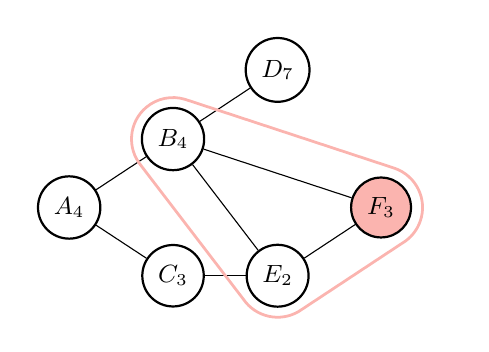
\begin{tikzpicture}[transform shape]
  \matrix[row sep=0.05cm,column sep=0.5cm] {
    % First line
                                                             &
                                                             &
    \node (d2)   [var, minimum size=0.7cm] {$D_7$};  &
                                                             &
                                                            \\
    % Second line
                                                             &
    \node (b2)   [var, minimum size=0.7cm] {$B_4$};          &
                                                             &
                                                             &
                                                            \\
    % Third line
    \node (a2) [var, minimum size=0.7cm] {$A_4$};            &
                                                             &
                                                             &
    \node (f2) [var, minimum size=0.7cm, fill=F] {$F_3$};    &
                                                            \\
    % Forth line
                                                             &
    \node (c2)   [var, minimum size=0.7cm] {$C_3$};          &
    \node (e2)   [var, minimum size=0.7cm] {$E_2$};          &
                                                             &
                                                            \\
  };

  \draw (a2) edge (b2);
  \draw (a2) edge (c2);
  %\draw (b2) edge (c2);
  \draw (b2) edge (d2);
  \draw (b2) edge (f2);
  \draw (b2) edge (e2);
  \draw (c2) edge (e2);
  \draw (e2) edge (f2);

  %\path (b1) -- node[anchor=center,xshift=-0.25cm,yshift=-0.1cm] (bc) {$\rightarrow$} (c1);

  \draw[F,line width=1pt] \convexpath{b2,f2,e2}{15pt};
  %\draw[D,line width=1pt] \convexpath{b2,d2}{15pt};
  %\draw[E,line width=1pt] \convexpath{b2,e2,c2}{15pt};
  %\draw[C,line width=1pt] \convexpath{a2,b2,c2}{15pt};

\end{tikzpicture}
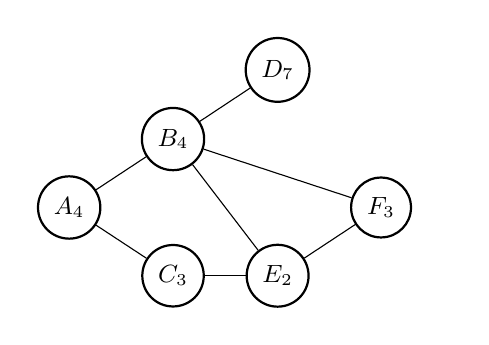
\begin{tikzpicture}[transform shape]

  \matrix[row sep=0.05cm,column sep=0.5cm] {
    % First line
                                                     &
                                                     &
    \node (d1)   [var, minimum size=0.7cm] {$D_7$};  &
                                                     &
                                                    \\
    % Second line
                                                     &
    \node (b1)   [var, minimum size=0.7cm] {$B_4$};  &
                                                     &
                                                     &
                                                    \\
    % Third line
    \node (a1) [var, minimum size=0.7cm] {$A_4$};    &
                                                     &
                                                     &
    \node (f1) [var, minimum size=0.7cm] {$F_3$};    &
                                                    \\
    % Forth line
                                                     &
    \node (c1)   [var, minimum size=0.7cm] {$C_3$};  &
    \node (e1)   [var, minimum size=0.7cm] {$E_2$};  &
                                                     &
                                                    \\
  };

  \draw (a1) edge (b1);
  \draw (a1) edge (c1);
  %\draw (b1) edge (c1);
  \draw (b1) edge (d1);
  \draw (b1) edge (f1);
  \draw (b1) edge (e1);
  \draw (c1) edge (e1);
  \draw (e1) edge (f1);

  %\draw[F,line width=1pt] \convexpath{b1,f1,e1}{15pt};
  %\draw[D,line width=1pt] \convexpath{b1,d1}{15pt};
  %\draw[E,line width=1pt] \convexpath{b1,e1,c1}{15pt};
  %\draw[C,line width=1pt] \convexpath{a1,b1,c1}{15pt};

\end{tikzpicture}

\end{frame}

%------------------------------------------------------------------------------
%%
%------------------------------------------------------------------------------

\begin{frame}[fragile]{Triangulation: Min-fill Algorithm}

\centering

{\footnotesize 
  Copy the cluster with the added edges to the right graph\\
  \textit{only if} it is not contained inside an already copied cluster.
}

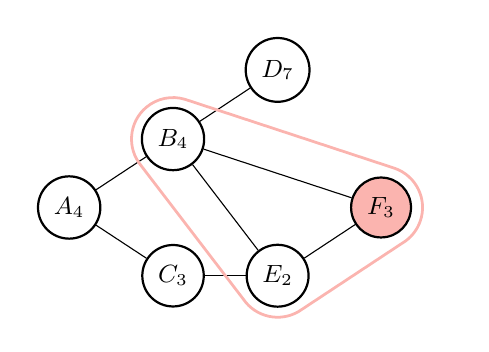
\begin{tikzpicture}[transform shape]
  \matrix[row sep=0.05cm,column sep=0.5cm] {
    % First line
                                                             &
                                                             &
    \node (d2)   [var, minimum size=0.7cm] {$D_7$};  &
                                                             &
                                                            \\
    % Second line
                                                             &
    \node (b2)   [var, minimum size=0.7cm] {$B_4$};          &
                                                             &
                                                             &
                                                            \\
    % Third line
    \node (a2) [var, minimum size=0.7cm] {$A_4$};            &
                                                             &
                                                             &
    \node (f2) [var, minimum size=0.7cm, fill=F] {$F_3$};    &
                                                            \\
    % Forth line
                                                             &
    \node (c2)   [var, minimum size=0.7cm] {$C_3$};          &
    \node (e2)   [var, minimum size=0.7cm] {$E_2$};          &
                                                             &
                                                            \\
  };

  \draw (a2) edge (b2);
  \draw (a2) edge (c2);
  %\draw (b2) edge (c2);
  \draw (b2) edge (d2);
  \draw (b2) edge (f2);
  \draw (b2) edge (e2);
  \draw (c2) edge (e2);
  \draw (e2) edge (f2);

  %\path (b1) -- node[anchor=center,xshift=-0.25cm,yshift=-0.1cm] (bc) {$\rightarrow$} (c1);

  \draw[F,line width=1pt] \convexpath{b2,f2,e2}{15pt};
  %\draw[D,line width=1pt] \convexpath{b2,d2}{15pt};
  %\draw[E,line width=1pt] \convexpath{b2,e2,c2}{15pt};
  %\draw[C,line width=1pt] \convexpath{a2,b2,c2}{15pt};

\end{tikzpicture}
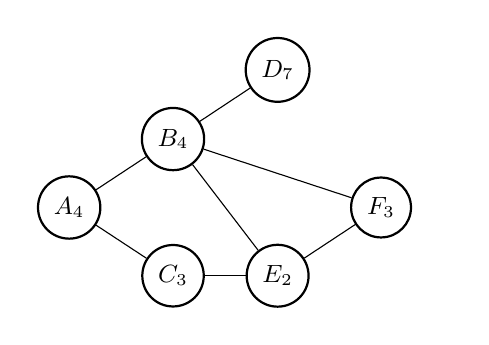
\begin{tikzpicture}[transform shape]

  \matrix[row sep=0.05cm,column sep=0.5cm] {
    % First line
                                                     &
                                                     &
    \node (d1)   [var, minimum size=0.7cm] {$D_7$};  &
                                                     &
                                                    \\
    % Second line
                                                     &
    \node (b1)   [var, minimum size=0.7cm] {$B_4$};  &
                                                     &
                                                     &
                                                    \\
    % Third line
    \node (a1) [var, minimum size=0.7cm] {$A_4$};    &
                                                     &
                                                     &
    \node (f1) [var, minimum size=0.7cm] {$F_3$};    &
                                                    \\
    % Forth line
                                                     &
    \node (c1)   [var, minimum size=0.7cm] {$C_3$};  &
    \node (e1)   [var, minimum size=0.7cm] {$E_2$};  &
                                                     &
                                                    \\
  };

  \draw (a1) edge (b1);
  \draw (a1) edge (c1);
  %\draw (b1) edge (c1);
  \draw (b1) edge (d1);
  \draw (b1) edge (f1);
  \draw (b1) edge (e1);
  \draw (c1) edge (e1);
  \draw (e1) edge (f1);

  %\draw[F,line width=1pt] \convexpath{b1,f1,e1}{15pt};
  %\draw[D,line width=1pt] \convexpath{b1,d1}{15pt};
  %\draw[E,line width=1pt] \convexpath{b1,e1,c1}{15pt};
  %\draw[C,line width=1pt] \convexpath{a1,b1,c1}{15pt};

\end{tikzpicture}

\end{frame}

%------------------------------------------------------------------------------
%%
%------------------------------------------------------------------------------

\begin{frame}[fragile]{Triangulation: Min-fill Algorithm}

\centering

{\footnotesize 
  Copy the cluster with the added edges to the right graph\\
  \textit{only if} it is not contained inside an already copied cluster.
}

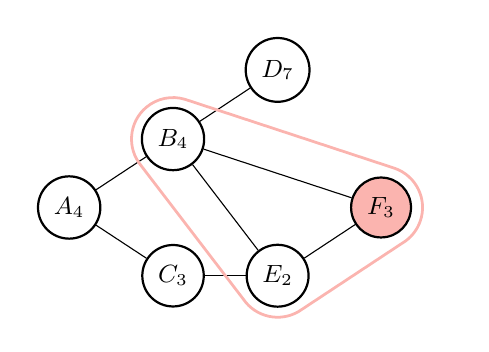
\begin{tikzpicture}[transform shape]
  \matrix[row sep=0.05cm,column sep=0.5cm] {
    % First line
                                                             &
                                                             &
    \node (d2)   [var, minimum size=0.7cm] {$D_7$};  &
                                                             &
                                                            \\
    % Second line
                                                             &
    \node (b2)   [var, minimum size=0.7cm] {$B_4$};          &
                                                             &
                                                             &
                                                            \\
    % Third line
    \node (a2) [var, minimum size=0.7cm] {$A_4$};            &
                                                             &
                                                             &
    \node (f2) [var, minimum size=0.7cm, fill=F] {$F_3$};    &
                                                            \\
    % Forth line
                                                             &
    \node (c2)   [var, minimum size=0.7cm] {$C_3$};          &
    \node (e2)   [var, minimum size=0.7cm] {$E_2$};          &
                                                             &
                                                            \\
  };

  \draw (a2) edge (b2);
  \draw (a2) edge (c2);
  %\draw (b2) edge (c2);
  \draw (b2) edge (d2);
  \draw (b2) edge (f2);
  \draw (b2) edge (e2);
  \draw (c2) edge (e2);
  \draw (e2) edge (f2);

  %\path (b1) -- node[anchor=center,xshift=-0.25cm,yshift=-0.1cm] (bc) {$\rightarrow$} (c1);

  \draw[F,line width=1pt] \convexpath{b2,f2,e2}{15pt};
  %\draw[D,line width=1pt] \convexpath{b2,d2}{15pt};
  %\draw[E,line width=1pt] \convexpath{b2,e2,c2}{15pt};
  %\draw[C,line width=1pt] \convexpath{a2,b2,c2}{15pt};

\end{tikzpicture}
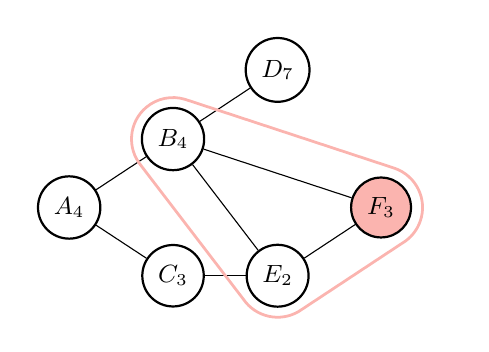
\begin{tikzpicture}[transform shape]

  \matrix[row sep=0.05cm,column sep=0.5cm] {
    % First line
                                                           &
                                                           &
    \node (d1)   [var, minimum size=0.7cm] {$D_7$};        &
                                                           &
                                                          \\
    % Second line
                                                           &
    \node (b1)   [var, minimum size=0.7cm] {$B_4$};        &
                                                           &
                                                           &
                                                          \\
    % Third line
    \node (a1) [var, minimum size=0.7cm] {$A_4$};          &
                                                           &
                                                           &
    \node (f1) [var, minimum size=0.7cm, fill=F] {$F_3$};  &
                                                          \\
    % Forth line
                                                           &
    \node (c1)   [var, minimum size=0.7cm] {$C_3$};        &
    \node (e1)   [var, minimum size=0.7cm] {$E_2$};        &
                                                           &
                                                          \\
  };

  \draw (a1) edge (b1);
  \draw (a1) edge (c1);
  %\draw (b1) edge (c1);
  \draw (b1) edge (d1);
  \draw (b1) edge (f1);
  \draw (b1) edge (e1);
  \draw (c1) edge (e1);
  \draw (e1) edge (f1);

  \draw[F,line width=1pt] \convexpath{b1,f1,e1}{15pt};
  %\draw[D,line width=1pt] \convexpath{b1,d1}{15pt};
  %\draw[E,line width=1pt] \convexpath{b1,e1,c1}{15pt};
  %\draw[C,line width=1pt] \convexpath{a1,b1,c1}{15pt};

\end{tikzpicture}

\end{frame}

%------------------------------------------------------------------------------
%%
%------------------------------------------------------------------------------

\begin{frame}[fragile]{Triangulation: Min-fill Algorithm}

\centering

{\footnotesize Remove $F$ from the left graph.}

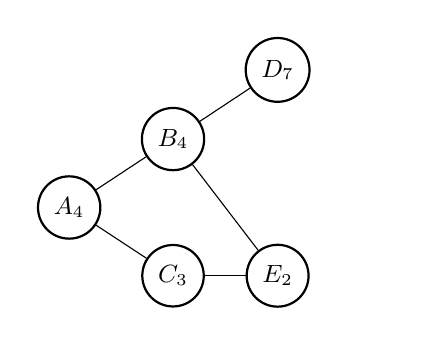
\begin{tikzpicture}[transform shape]
  \matrix[row sep=0.05cm,column sep=0.5cm] {
    % First line
                                                     &
                                                     &
    \node (d2)   [var, minimum size=0.7cm] {$D_7$};  &
                                                     &
                                                    \\
    % Second line
                                                     &
    \node (b2)   [var, minimum size=0.7cm] {$B_4$};  &
                                                     &
                                                     &
                                                    \\
    % Third line
    \node (a2) [var, minimum size=0.7cm] {$A_4$};    &
                                                     &
                                                     &
                                                     &
                                                    \\
    % Forth line
                                                     &
    \node (c2)   [var, minimum size=0.7cm] {$C_3$};  &
    \node (e2)   [var, minimum size=0.7cm] {$E_2$};  &
                                                     &
                                                    \\
  };

  \draw (a2) edge (b2);
  \draw (a2) edge (c2);
  %\draw (b2) edge (c2);
  \draw (b2) edge (d2);
  %\draw (b2) edge (f2);
  \draw (b2) edge (e2);
  \draw (c2) edge (e2);
  %\draw (e2) edge (f2);

  %\path (b1) -- node[anchor=center,xshift=-0.25cm,yshift=-0.1cm] (bc) {$\rightarrow$} (c1);

  %\draw[F,line width=1pt] \convexpath{b2,f2,e2}{15pt};
  %\draw[D,line width=1pt] \convexpath{b2,d2}{15pt};
  %\draw[E,line width=1pt] \convexpath{b2,e2,c2}{15pt};
  %\draw[C,line width=1pt] \convexpath{a2,b2,c2}{15pt};

\end{tikzpicture}
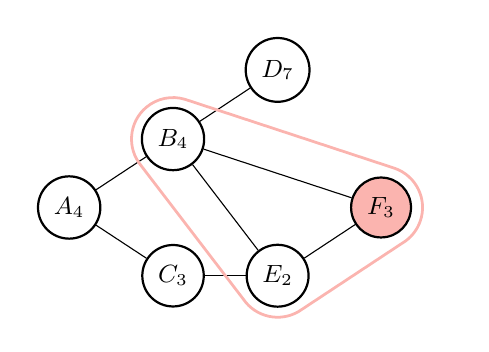
\begin{tikzpicture}[transform shape]

  \matrix[row sep=0.05cm,column sep=0.5cm] {
    % First line
                                                           &
                                                           &
    \node (d1)   [var, minimum size=0.7cm] {$D_7$};        &
                                                           &
                                                          \\
    % Second line
                                                           &
    \node (b1)   [var, minimum size=0.7cm] {$B_4$};        &
                                                           &
                                                           &
                                                          \\
    % Third line
    \node (a1) [var, minimum size=0.7cm] {$A_4$};          &
                                                           &
                                                           &
    \node (f1) [var, minimum size=0.7cm, fill=F] {$F_3$};  &
                                                          \\
    % Forth line
                                                           &
    \node (c1)   [var, minimum size=0.7cm] {$C_3$};        &
    \node (e1)   [var, minimum size=0.7cm] {$E_2$};        &
                                                           &
                                                          \\
  };

  \draw (a1) edge (b1);
  \draw (a1) edge (c1);
  %\draw (b1) edge (c1);
  \draw (b1) edge (d1);
  \draw (b1) edge (f1);
  \draw (b1) edge (e1);
  \draw (c1) edge (e1);
  \draw (e1) edge (f1);

  \draw[F,line width=1pt] \convexpath{b1,f1,e1}{15pt};
  %\draw[D,line width=1pt] \convexpath{b1,d1}{15pt};
  %\draw[E,line width=1pt] \convexpath{b1,e1,c1}{15pt};
  %\draw[C,line width=1pt] \convexpath{a1,b1,c1}{15pt};

\end{tikzpicture}

%\begin{center}
%  \scriptsize
%  \begin{tabular}{ccc}
%  \toprule
%  \textbf{Eliminated Vertex} & \textbf{Induced Cluster} & \textbf{Edges Added} \\
%  \midrule
%  F                 & BEF             & none        \\
%  \bottomrule
%  \end{tabular}
%\end{center}
%\vfill

\end{frame}

%------------------------------------------------------------------------------
%%
%------------------------------------------------------------------------------

\begin{frame}[fragile]{Triangulation: Min-fill Algorithm}

\centering

{\footnotesize Repeat until there are no nodes left in the left graph.}

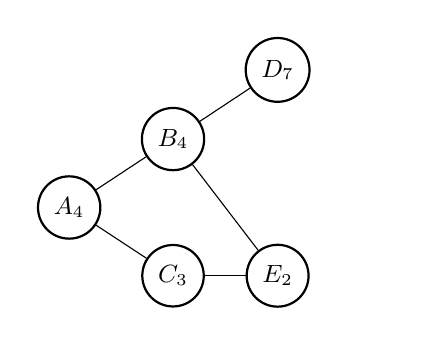
\begin{tikzpicture}[transform shape]
  \matrix[row sep=0.05cm,column sep=0.5cm] {
    % First line
                                                     &
                                                     &
    \node (d2)   [var, minimum size=0.7cm] {$D_7$};  &
                                                     &
                                                    \\
    % Second line
                                                     &
    \node (b2)   [var, minimum size=0.7cm] {$B_4$};  &
                                                     &
                                                     &
                                                    \\
    % Third line
    \node (a2) [var, minimum size=0.7cm] {$A_4$};    &
                                                     &
                                                     &
                                                     &
                                                    \\
    % Forth line
                                                     &
    \node (c2)   [var, minimum size=0.7cm] {$C_3$};  &
    \node (e2)   [var, minimum size=0.7cm] {$E_2$};  &
                                                     &
                                                    \\
  };

  \draw (a2) edge (b2);
  \draw (a2) edge (c2);
  %\draw (b2) edge (c2);
  \draw (b2) edge (d2);
  %\draw (b2) edge (f2);
  \draw (b2) edge (e2);
  \draw (c2) edge (e2);
  %\draw (e2) edge (f2);

  %\path (b1) -- node[anchor=center,xshift=-0.25cm,yshift=-0.1cm] (bc) {$\rightarrow$} (c1);

  %\draw[F,line width=1pt] \convexpath{b2,f2,e2}{15pt};
  %\draw[D,line width=1pt] \convexpath{b2,d2}{15pt};
  %\draw[E,line width=1pt] \convexpath{b2,e2,c2}{15pt};
  %\draw[C,line width=1pt] \convexpath{a2,b2,c2}{15pt};

\end{tikzpicture}
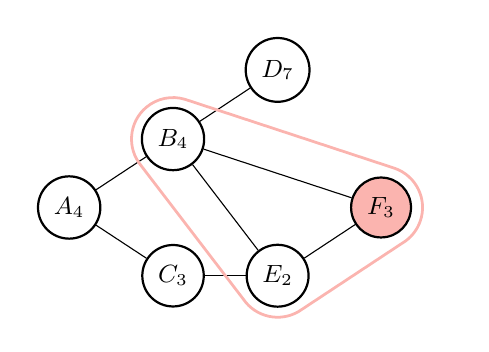
\begin{tikzpicture}[transform shape]

  \matrix[row sep=0.05cm,column sep=0.5cm] {
    % First line
                                                           &
                                                           &
    \node (d1)   [var, minimum size=0.7cm] {$D_7$};        &
                                                           &
                                                          \\
    % Second line
                                                           &
    \node (b1)   [var, minimum size=0.7cm] {$B_4$};        &
                                                           &
                                                           &
                                                          \\
    % Third line
    \node (a1) [var, minimum size=0.7cm] {$A_4$};          &
                                                           &
                                                           &
    \node (f1) [var, minimum size=0.7cm, fill=F] {$F_3$};  &
                                                          \\
    % Forth line
                                                           &
    \node (c1)   [var, minimum size=0.7cm] {$C_3$};        &
    \node (e1)   [var, minimum size=0.7cm] {$E_2$};        &
                                                           &
                                                          \\
  };

  \draw (a1) edge (b1);
  \draw (a1) edge (c1);
  %\draw (b1) edge (c1);
  \draw (b1) edge (d1);
  \draw (b1) edge (f1);
  \draw (b1) edge (e1);
  \draw (c1) edge (e1);
  \draw (e1) edge (f1);

  \draw[F,line width=1pt] \convexpath{b1,f1,e1}{15pt};
  %\draw[D,line width=1pt] \convexpath{b1,d1}{15pt};
  %\draw[E,line width=1pt] \convexpath{b1,e1,c1}{15pt};
  %\draw[C,line width=1pt] \convexpath{a1,b1,c1}{15pt};

\end{tikzpicture}

%\begin{center}
%  \scriptsize
%  \begin{tabular}{ccc}
%  \toprule
%  \textbf{Eliminated Vertex} & \textbf{Induced Cluster} & \textbf{Edges Added} \\
%  \midrule
%  F                 & BEF             & none        \\
%  \bottomrule
%  \end{tabular}
%\end{center}
%\vfill

\end{frame}

%------------------------------------------------------------------------------
%%
%------------------------------------------------------------------------------

\begin{frame}[fragile]{Triangulation: Min-fill Algorithm}

\centering

{\footnotesize
  Node selection criterion: 
  {\scriptsize
  \begin{itemize}
    \item Select the node that causes the \textit{least} number of edges to be
      added in the cluster.
    \item Break ties by choosing the node that induces the cluster with the
      \textit{smallest} state space size.
  \end{itemize}
  }
}

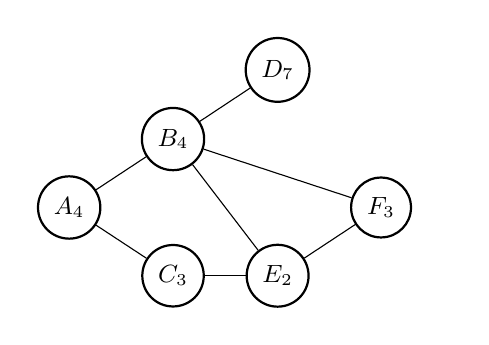
\begin{tikzpicture}[transform shape]

  \matrix[row sep=0.05cm,column sep=0.5cm] {
    % First line
                                                     &
                                                     &
    \node (d1)   [var, minimum size=0.7cm] {$D_7$};  &
                                                     &
                                                    \\
    % Second line
                                                     &
    \node (b1)   [var, minimum size=0.7cm] {$B_4$};  &
                                                     &
                                                     &
                                                    \\
    % Third line
    \node (a1) [var, minimum size=0.7cm] {$A_4$};    &
                                                     &
                                                     &
    \node (f1) [var, minimum size=0.7cm] {$F_3$};    &
                                                    \\
    % Forth line
                                                     &
    \node (c1)   [var, minimum size=0.7cm] {$C_3$};  &
    \node (e1)   [var, minimum size=0.7cm] {$E_2$};  &
                                                     &
                                                    \\
  };

  \draw (a1) edge (b1);
  \draw (a1) edge (c1);
  %\draw (b1) edge (c1);
  \draw (b1) edge (d1);
  \draw (b1) edge (f1);
  \draw (b1) edge (e1);
  \draw (c1) edge (e1);
  \draw (e1) edge (f1);

  %\draw[F,line width=1pt] \convexpath{b1,f1,e1}{15pt};
  %\draw[D,line width=1pt] \convexpath{b1,d1}{15pt};
  %\draw[E,line width=1pt] \convexpath{b1,e1,c1}{15pt};
  %\draw[C,line width=1pt] \convexpath{a1,b1,c1}{15pt};

\end{tikzpicture}
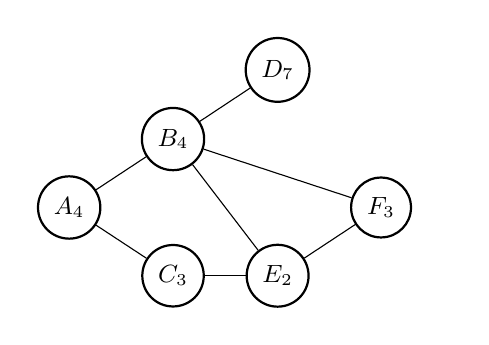
\begin{tikzpicture}[transform shape]
  \matrix[row sep=0.05cm,column sep=0.5cm] {
    % First line
                                                     &
                                                     &
    \node (d2)   [var, minimum size=0.7cm] {$D_7$};  &
                                                     &
                                                    \\
    % Second line
                                                     &
    \node (b2)   [var, minimum size=0.7cm] {$B_4$};  &
                                                     &
                                                     &
                                                    \\
    % Third line
    \node (a2) [var, minimum size=0.7cm] {$A_4$};    &
                                                     &
                                                     &
    \node (f2) [var, minimum size=0.7cm] {$F_3$};    &
                                                    \\
    % Forth line
                                                     &
    \node (c2)   [var, minimum size=0.7cm] {$C_3$};  &
    \node (e2)   [var, minimum size=0.7cm] {$E_2$};  &
                                                     &
                                                    \\
  };

  \draw (a2) edge (b2);
  \draw (a2) edge (c2);
  %\draw (b2) edge (c2);
  \draw (b2) edge (d2);
  \draw (b2) edge (f2);
  \draw (b2) edge (e2);
  \draw (c2) edge (e2);
  \draw (e2) edge (f2);

  %\path (b1) -- node[anchor=center,xshift=-0.25cm,yshift=-0.1cm] (bc) {$\rightarrow$} (c1);

  %\draw[F,line width=1pt] \convexpath{b2,f2,e2}{15pt};
  %\draw[D,line width=1pt] \convexpath{b2,d2}{15pt};
  %\draw[E,line width=1pt] \convexpath{b2,e2,c2}{15pt};
  %\draw[C,line width=1pt] \convexpath{a2,b2,c2}{15pt};

\end{tikzpicture}

\end{frame}

%------------------------------------------------------------------------------
%%
%------------------------------------------------------------------------------

\begin{frame}[fragile]{Triangulation: Min-fill Algorithm}

\centering

{\footnotesize
  Selecting which node causes the least $\#$ of edges to be added in the
  induced cluster?
}

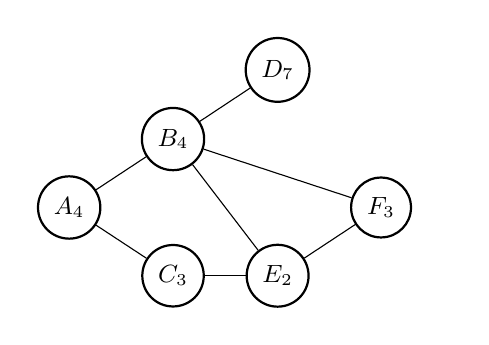
\begin{tikzpicture}[transform shape]

  \matrix[row sep=0.05cm,column sep=0.5cm] {
    % First line
                                                     &
                                                     &
    \node (d1)   [var, minimum size=0.7cm] {$D_7$};  &
                                                     &
                                                    \\
    % Second line
                                                     &
    \node (b1)   [var, minimum size=0.7cm] {$B_4$};  &
                                                     &
                                                     &
                                                    \\
    % Third line
    \node (a1) [var, minimum size=0.7cm] {$A_4$};    &
                                                     &
                                                     &
    \node (f1) [var, minimum size=0.7cm] {$F_3$};    &
                                                    \\
    % Forth line
                                                     &
    \node (c1)   [var, minimum size=0.7cm] {$C_3$};  &
    \node (e1)   [var, minimum size=0.7cm] {$E_2$};  &
                                                     &
                                                    \\
  };

  \draw (a1) edge (b1);
  \draw (a1) edge (c1);
  %\draw (b1) edge (c1);
  \draw (b1) edge (d1);
  \draw (b1) edge (f1);
  \draw (b1) edge (e1);
  \draw (c1) edge (e1);
  \draw (e1) edge (f1);

  %\draw[F,line width=1pt] \convexpath{b1,f1,e1}{15pt};
  %\draw[D,line width=1pt] \convexpath{b1,d1}{15pt};
  %\draw[E,line width=1pt] \convexpath{b1,e1,c1}{15pt};
  %\draw[C,line width=1pt] \convexpath{a1,b1,c1}{15pt};

\end{tikzpicture}
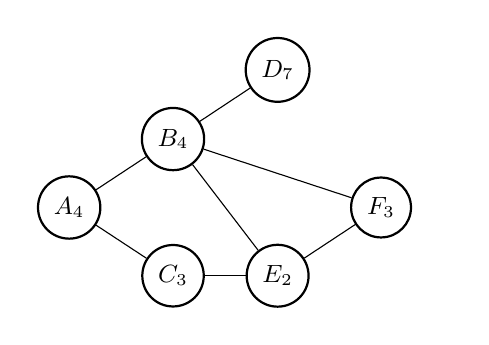
\begin{tikzpicture}[transform shape]
  \matrix[row sep=0.05cm,column sep=0.5cm] {
    % First line
                                                     &
                                                     &
    \node (d2)   [var, minimum size=0.7cm] {$D_7$};  &
                                                     &
                                                    \\
    % Second line
                                                     &
    \node (b2)   [var, minimum size=0.7cm] {$B_4$};  &
                                                     &
                                                     &
                                                    \\
    % Third line
    \node (a2) [var, minimum size=0.7cm] {$A_4$};    &
                                                     &
                                                     &
    \node (f2) [var, minimum size=0.7cm] {$F_3$};    &
                                                    \\
    % Forth line
                                                     &
    \node (c2)   [var, minimum size=0.7cm] {$C_3$};  &
    \node (e2)   [var, minimum size=0.7cm] {$E_2$};  &
                                                     &
                                                    \\
  };

  \draw (a2) edge (b2);
  \draw (a2) edge (c2);
  %\draw (b2) edge (c2);
  \draw (b2) edge (d2);
  \draw (b2) edge (f2);
  \draw (b2) edge (e2);
  \draw (c2) edge (e2);
  \draw (e2) edge (f2);

  %\path (b1) -- node[anchor=center,xshift=-0.25cm,yshift=-0.1cm] (bc) {$\rightarrow$} (c1);

  %\draw[F,line width=1pt] \convexpath{b2,f2,e2}{15pt};
  %\draw[D,line width=1pt] \convexpath{b2,d2}{15pt};
  %\draw[E,line width=1pt] \convexpath{b2,e2,c2}{15pt};
  %\draw[C,line width=1pt] \convexpath{a2,b2,c2}{15pt};

\end{tikzpicture}

\end{frame}

%------------------------------------------------------------------------------
%% 
%------------------------------------------------------------------------------

\begin{frame}[fragile]{Triangulation: Min-fill Algorithm}

\centering

{\footnotesize Tie.}

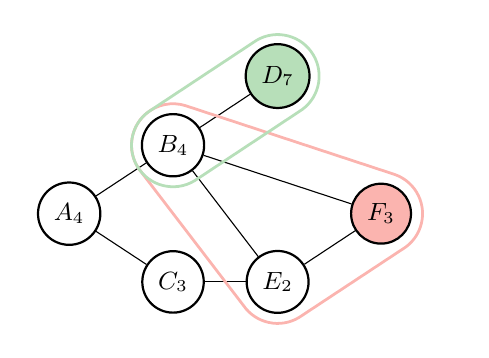
\begin{tikzpicture}[transform shape]
  \matrix[row sep=0.05cm,column sep=0.5cm] {
    % First line
                                                             &
                                                             &
    \node (d2)   [var, minimum size=0.7cm, fill=D] {$D_7$};  &
                                                             &
                                                            \\
    % Second line
                                                             &
    \node (b2)   [var, minimum size=0.7cm] {$B_4$};          &
                                                             &
                                                             &
                                                            \\
    % Third line
    \node (a2) [var, minimum size=0.7cm] {$A_4$};            &
                                                             &
                                                             &
    \node (f2) [var, minimum size=0.7cm, fill=F] {$F_3$};    &
                                                            \\
    % Forth line
                                                             &
    \node (c2)   [var, minimum size=0.7cm] {$C_3$};          &
    \node (e2)   [var, minimum size=0.7cm] {$E_2$};          &
                                                             &
                                                            \\
  };

  \draw (a2) edge (b2);
  \draw (a2) edge (c2);
  %\draw (b2) edge (c2);
  \draw (b2) edge (d2);
  \draw (b2) edge (f2);
  \draw (b2) edge (e2);
  \draw (c2) edge (e2);
  \draw (e2) edge (f2);

  %\path (b1) -- node[anchor=center,xshift=-0.25cm,yshift=-0.1cm] (bc) {$\rightarrow$} (c1);

  \draw[F,line width=1pt] \convexpath{b2,f2,e2}{15pt};
  \draw[D,line width=1pt] \convexpath{b2,d2}{15pt};
  %\draw[E,line width=1pt] \convexpath{b2,e2,c2}{15pt};
  %\draw[C,line width=1pt] \convexpath{a2,b2,c2}{15pt};

\end{tikzpicture}
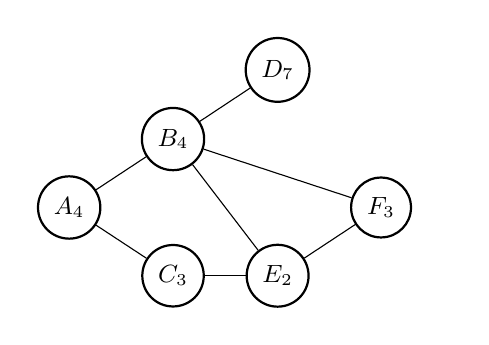
\begin{tikzpicture}[transform shape]

  \matrix[row sep=0.05cm,column sep=0.5cm] {
    % First line
                                                     &
                                                     &
    \node (d1)   [var, minimum size=0.7cm] {$D_7$};  &
                                                     &
                                                    \\
    % Second line
                                                     &
    \node (b1)   [var, minimum size=0.7cm] {$B_4$};  &
                                                     &
                                                     &
                                                    \\
    % Third line
    \node (a1) [var, minimum size=0.7cm] {$A_4$};    &
                                                     &
                                                     &
    \node (f1) [var, minimum size=0.7cm] {$F_3$};    &
                                                    \\
    % Forth line
                                                     &
    \node (c1)   [var, minimum size=0.7cm] {$C_3$};  &
    \node (e1)   [var, minimum size=0.7cm] {$E_2$};  &
                                                     &
                                                    \\
  };

  \draw (a1) edge (b1);
  \draw (a1) edge (c1);
  %\draw (b1) edge (c1);
  \draw (b1) edge (d1);
  \draw (b1) edge (f1);
  \draw (b1) edge (e1);
  \draw (c1) edge (e1);
  \draw (e1) edge (f1);

  %\draw[F,line width=1pt] \convexpath{b1,f1,e1}{15pt};
  %\draw[D,line width=1pt] \convexpath{b1,d1}{15pt};
  %\draw[E,line width=1pt] \convexpath{b1,e1,c1}{15pt};
  %\draw[C,line width=1pt] \convexpath{a1,b1,c1}{15pt};

\end{tikzpicture}

\end{frame}

%------------------------------------------------------------------------------
%% 
%------------------------------------------------------------------------------

\begin{frame}[fragile]{Triangulation: Min-fill Algorithm}

\centering

{\footnotesize Then which of the two clusters has a smaller state space size?}

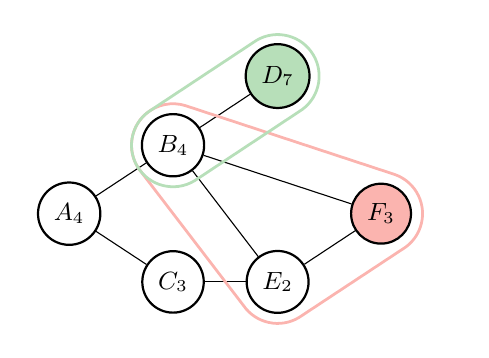
\begin{tikzpicture}[transform shape]
  \matrix[row sep=0.05cm,column sep=0.5cm] {
    % First line
                                                             &
                                                             &
    \node (d2)   [var, minimum size=0.7cm, fill=D] {$D_7$};  &
                                                             &
                                                            \\
    % Second line
                                                             &
    \node (b2)   [var, minimum size=0.7cm] {$B_4$};          &
                                                             &
                                                             &
                                                            \\
    % Third line
    \node (a2) [var, minimum size=0.7cm] {$A_4$};            &
                                                             &
                                                             &
    \node (f2) [var, minimum size=0.7cm, fill=F] {$F_3$};    &
                                                            \\
    % Forth line
                                                             &
    \node (c2)   [var, minimum size=0.7cm] {$C_3$};          &
    \node (e2)   [var, minimum size=0.7cm] {$E_2$};          &
                                                             &
                                                            \\
  };

  \draw (a2) edge (b2);
  \draw (a2) edge (c2);
  %\draw (b2) edge (c2);
  \draw (b2) edge (d2);
  \draw (b2) edge (f2);
  \draw (b2) edge (e2);
  \draw (c2) edge (e2);
  \draw (e2) edge (f2);

  %\path (b1) -- node[anchor=center,xshift=-0.25cm,yshift=-0.1cm] (bc) {$\rightarrow$} (c1);

  \draw[F,line width=1pt] \convexpath{b2,f2,e2}{15pt};
  \draw[D,line width=1pt] \convexpath{b2,d2}{15pt};
  %\draw[E,line width=1pt] \convexpath{b2,e2,c2}{15pt};
  %\draw[C,line width=1pt] \convexpath{a2,b2,c2}{15pt};

\end{tikzpicture}
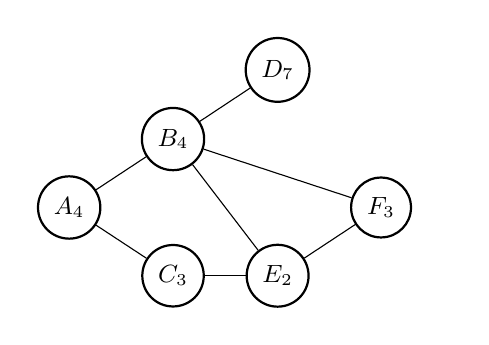
\begin{tikzpicture}[transform shape]

  \matrix[row sep=0.05cm,column sep=0.5cm] {
    % First line
                                                     &
                                                     &
    \node (d1)   [var, minimum size=0.7cm] {$D_7$};  &
                                                     &
                                                    \\
    % Second line
                                                     &
    \node (b1)   [var, minimum size=0.7cm] {$B_4$};  &
                                                     &
                                                     &
                                                    \\
    % Third line
    \node (a1) [var, minimum size=0.7cm] {$A_4$};    &
                                                     &
                                                     &
    \node (f1) [var, minimum size=0.7cm] {$F_3$};    &
                                                    \\
    % Forth line
                                                     &
    \node (c1)   [var, minimum size=0.7cm] {$C_3$};  &
    \node (e1)   [var, minimum size=0.7cm] {$E_2$};  &
                                                     &
                                                    \\
  };

  \draw (a1) edge (b1);
  \draw (a1) edge (c1);
  %\draw (b1) edge (c1);
  \draw (b1) edge (d1);
  \draw (b1) edge (f1);
  \draw (b1) edge (e1);
  \draw (c1) edge (e1);
  \draw (e1) edge (f1);

  %\draw[F,line width=1pt] \convexpath{b1,f1,e1}{15pt};
  %\draw[D,line width=1pt] \convexpath{b1,d1}{15pt};
  %\draw[E,line width=1pt] \convexpath{b1,e1,c1}{15pt};
  %\draw[C,line width=1pt] \convexpath{a1,b1,c1}{15pt};

\end{tikzpicture}

\end{frame}

%------------------------------------------------------------------------------
%%
%------------------------------------------------------------------------------

\begin{frame}[fragile]{Triangulation: Min-fill Algorithm}

\centering

{\footnotesize $ \lvert BEF \rvert < \lvert BD \rvert $, therefore $F$ wins.}

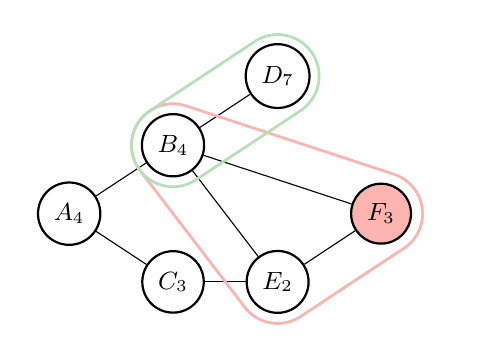
\begin{tikzpicture}[transform shape]
  \matrix[row sep=0.05cm,column sep=0.5cm] {
    % First line
                                                             &
                                                             &
    \node (d2)   [var, minimum size=0.7cm] {$D_7$};  &
                                                             &
                                                            \\
    % Second line
                                                             &
    \node (b2)   [var, minimum size=0.7cm] {$B_4$};          &
                                                             &
                                                             &
                                                            \\
    % Third line
    \node (a2) [var, minimum size=0.7cm] {$A_4$};            &
                                                             &
                                                             &
    \node (f2) [var, minimum size=0.7cm, fill=F] {$F_3$};    &
                                                            \\
    % Forth line
                                                             &
    \node (c2)   [var, minimum size=0.7cm] {$C_3$};          &
    \node (e2)   [var, minimum size=0.7cm] {$E_2$};          &
                                                             &
                                                            \\
  };

  \draw (a2) edge (b2);
  \draw (a2) edge (c2);
  %\draw (b2) edge (c2);
  \draw (b2) edge (d2);
  \draw (b2) edge (f2);
  \draw (b2) edge (e2);
  \draw (c2) edge (e2);
  \draw (e2) edge (f2);

  %\path (b1) -- node[anchor=center,xshift=-0.25cm,yshift=-0.1cm] (bc) {$\rightarrow$} (c1);

  \draw[F,line width=1pt] \convexpath{b2,f2,e2}{15pt};
  \draw[D,line width=1pt] \convexpath{b2,d2}{15pt};
  %\draw[E,line width=1pt] \convexpath{b2,e2,c2}{15pt};
  %\draw[C,line width=1pt] \convexpath{a2,b2,c2}{15pt};

\end{tikzpicture}
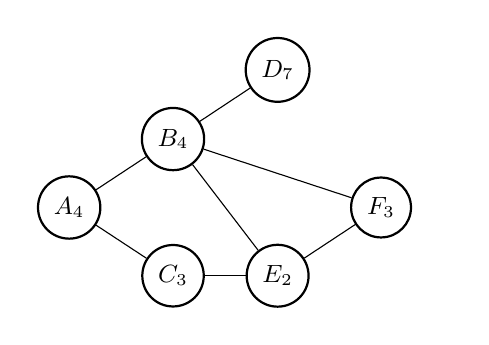
\begin{tikzpicture}[transform shape]

  \matrix[row sep=0.05cm,column sep=0.5cm] {
    % First line
                                                     &
                                                     &
    \node (d1)   [var, minimum size=0.7cm] {$D_7$};  &
                                                     &
                                                    \\
    % Second line
                                                     &
    \node (b1)   [var, minimum size=0.7cm] {$B_4$};  &
                                                     &
                                                     &
                                                    \\
    % Third line
    \node (a1) [var, minimum size=0.7cm] {$A_4$};    &
                                                     &
                                                     &
    \node (f1) [var, minimum size=0.7cm] {$F_3$};    &
                                                    \\
    % Forth line
                                                     &
    \node (c1)   [var, minimum size=0.7cm] {$C_3$};  &
    \node (e1)   [var, minimum size=0.7cm] {$E_2$};  &
                                                     &
                                                    \\
  };

  \draw (a1) edge (b1);
  \draw (a1) edge (c1);
  %\draw (b1) edge (c1);
  \draw (b1) edge (d1);
  \draw (b1) edge (f1);
  \draw (b1) edge (e1);
  \draw (c1) edge (e1);
  \draw (e1) edge (f1);

  %\draw[F,line width=1pt] \convexpath{b1,f1,e1}{15pt};
  %\draw[D,line width=1pt] \convexpath{b1,d1}{15pt};
  %\draw[E,line width=1pt] \convexpath{b1,e1,c1}{15pt};
  %\draw[C,line width=1pt] \convexpath{a1,b1,c1}{15pt};

\end{tikzpicture}
\end{frame}

%------------------------------------------------------------------------------
%%
%------------------------------------------------------------------------------

\begin{frame}[fragile]{Triangulation: Min-fill Algorithm}

\centering

{\footnotesize 
  Back to where we were.\\
  Repeat until there are no nodes left in the left graph.
}

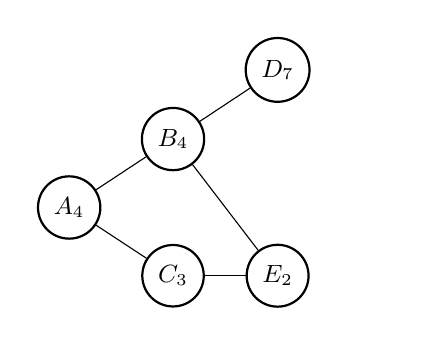
\begin{tikzpicture}[transform shape]
  \matrix[row sep=0.05cm,column sep=0.5cm] {
    % First line
                                                     &
                                                     &
    \node (d2)   [var, minimum size=0.7cm] {$D_7$};  &
                                                     &
                                                    \\
    % Second line
                                                     &
    \node (b2)   [var, minimum size=0.7cm] {$B_4$};  &
                                                     &
                                                     &
                                                    \\
    % Third line
    \node (a2) [var, minimum size=0.7cm] {$A_4$};    &
                                                     &
                                                     &
                                                     &
                                                    \\
    % Forth line
                                                     &
    \node (c2)   [var, minimum size=0.7cm] {$C_3$};  &
    \node (e2)   [var, minimum size=0.7cm] {$E_2$};  &
                                                     &
                                                    \\
  };

  \draw (a2) edge (b2);
  \draw (a2) edge (c2);
  %\draw (b2) edge (c2);
  \draw (b2) edge (d2);
  %\draw (b2) edge (f2);
  \draw (b2) edge (e2);
  \draw (c2) edge (e2);
  %\draw (e2) edge (f2);

  %\path (b1) -- node[anchor=center,xshift=-0.25cm,yshift=-0.1cm] (bc) {$\rightarrow$} (c1);

  %\draw[F,line width=1pt] \convexpath{b2,f2,e2}{15pt};
  %\draw[D,line width=1pt] \convexpath{b2,d2}{15pt};
  %\draw[E,line width=1pt] \convexpath{b2,e2,c2}{15pt};
  %\draw[C,line width=1pt] \convexpath{a2,b2,c2}{15pt};

\end{tikzpicture}
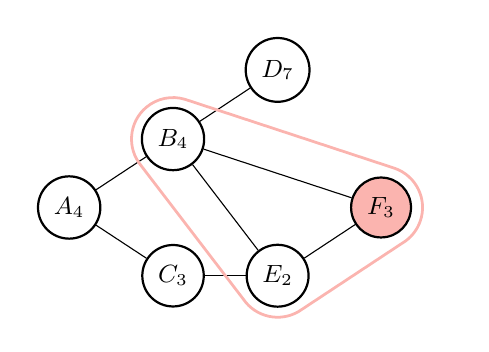
\begin{tikzpicture}[transform shape]

  \matrix[row sep=0.05cm,column sep=0.5cm] {
    % First line
                                                           &
                                                           &
    \node (d1)   [var, minimum size=0.7cm] {$D_7$};        &
                                                           &
                                                          \\
    % Second line
                                                           &
    \node (b1)   [var, minimum size=0.7cm] {$B_4$};        &
                                                           &
                                                           &
                                                          \\
    % Third line
    \node (a1) [var, minimum size=0.7cm] {$A_4$};          &
                                                           &
                                                           &
    \node (f1) [var, minimum size=0.7cm, fill=F] {$F_3$};  &
                                                          \\
    % Forth line
                                                           &
    \node (c1)   [var, minimum size=0.7cm] {$C_3$};        &
    \node (e1)   [var, minimum size=0.7cm] {$E_2$};        &
                                                           &
                                                          \\
  };

  \draw (a1) edge (b1);
  \draw (a1) edge (c1);
  %\draw (b1) edge (c1);
  \draw (b1) edge (d1);
  \draw (b1) edge (f1);
  \draw (b1) edge (e1);
  \draw (c1) edge (e1);
  \draw (e1) edge (f1);

  \draw[F,line width=1pt] \convexpath{b1,f1,e1}{15pt};
  %\draw[D,line width=1pt] \convexpath{b1,d1}{15pt};
  %\draw[E,line width=1pt] \convexpath{b1,e1,c1}{15pt};
  %\draw[C,line width=1pt] \convexpath{a1,b1,c1}{15pt};

\end{tikzpicture}

%\begin{center}
%  \scriptsize
%  \begin{tabular}{ccc}
%  \toprule
%  \textbf{Eliminated Vertex} & \textbf{Induced Cluster} & \textbf{Edges Added} \\
%  \midrule
%  F                 & BEF             & none        \\
%  \bottomrule
%  \end{tabular}
%\end{center}
%\vfill

\end{frame}

%------------------------------------------------------------------------------
%%
%------------------------------------------------------------------------------

\begin{frame}[fragile]{Triangulation: Min-fill Algorithm}

\centering

{\footnotesize
  Selecting which node causes the least $\#$ of edges to be added in the
  induced cluster?
}

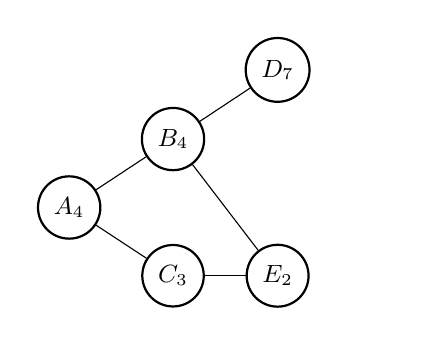
\begin{tikzpicture}[transform shape]
  \matrix[row sep=0.05cm,column sep=0.5cm] {
    % First line
                                                     &
                                                     &
    \node (d2)   [var, minimum size=0.7cm] {$D_7$};  &
                                                     &
                                                    \\
    % Second line
                                                     &
    \node (b2)   [var, minimum size=0.7cm] {$B_4$};  &
                                                     &
                                                     &
                                                    \\
    % Third line
    \node (a2) [var, minimum size=0.7cm] {$A_4$};    &
                                                     &
                                                     &
                                                     &
                                                    \\
    % Forth line
                                                     &
    \node (c2)   [var, minimum size=0.7cm] {$C_3$};  &
    \node (e2)   [var, minimum size=0.7cm] {$E_2$};  &
                                                     &
                                                    \\
  };

  \draw (a2) edge (b2);
  \draw (a2) edge (c2);
  %\draw (b2) edge (c2);
  \draw (b2) edge (d2);
  %\draw (b2) edge (f2);
  \draw (b2) edge (e2);
  \draw (c2) edge (e2);
  %\draw (e2) edge (f2);

  %\path (b1) -- node[anchor=center,xshift=-0.25cm,yshift=-0.1cm] (bc) {$\rightarrow$} (c1);

  %\draw[F,line width=1pt] \convexpath{b2,f2,e2}{15pt};
  %\draw[D,line width=1pt] \convexpath{b2,d2}{15pt};
  %\draw[E,line width=1pt] \convexpath{b2,e2,c2}{15pt};
  %\draw[C,line width=1pt] \convexpath{a2,b2,c2}{15pt};

\end{tikzpicture}
\begin{tikzpicture}[transform shape]

  \matrix[row sep=0.05cm,column sep=0.5cm] {
    % First line
                                                           &
                                                           &
    \node (d1)   [var, minimum size=0.7cm] {$D_7$};        &
                                                           &
                                                          \\
    % Second line
                                                           &
    \node (b1)   [var, minimum size=0.7cm] {$B_4$};        &
                                                           &
                                                           &
                                                          \\
    % Third line
    \node (a1) [var, minimum size=0.7cm] {$A_4$};          &
                                                           &
                                                           &
    \node (f1) [var, minimum size=0.7cm, fill=F] {$F_3$};  &
                                                          \\
    % Forth line
                                                           &
    \node (c1)   [var, minimum size=0.7cm] {$C_3$};        &
    \node (e1)   [var, minimum size=0.7cm] {$E_2$};        &
                                                           &
                                                          \\
  };

  \draw (a1) edge (b1);
  \draw (a1) edge (c1);
  %\draw (b1) edge (c1);
  \draw (b1) edge (d1);
  \draw (b1) edge (f1);
  \draw (b1) edge (e1);
  \draw (c1) edge (e1);
  \draw (e1) edge (f1);

  \draw[F,line width=1pt] \convexpath{b1,f1,e1}{15pt};
  %\draw[D,line width=1pt] \convexpath{b1,d1}{15pt};
  %\draw[E,line width=1pt] \convexpath{b1,e1,c1}{15pt};
  %\draw[C,line width=1pt] \convexpath{a1,b1,c1}{15pt};

\end{tikzpicture}

%\begin{center}
%  \scriptsize
%  \begin{tabular}{ccc}
%  \toprule
%  \textbf{Eliminated Vertex} & \textbf{Induced Cluster} & \textbf{Edges Added} \\
%  \midrule
%  F                 & BEF             & none        \\
%  \bottomrule
%  \end{tabular}
%\end{center}
%\vfill

\end{frame}

%------------------------------------------------------------------------------
%%
%------------------------------------------------------------------------------

\begin{frame}[fragile]{Triangulation: Min-fill Algorithm}

\centering

%{\footnotesize Text.}

\begin{tikzpicture}[transform shape]
  \matrix[row sep=0.05cm,column sep=0.5cm] {
    % First line
                                                             &
                                                             &
    \node (d2)   [var, minimum size=0.7cm, fill=D] {$D_7$};  &
                                                             &
                                                            \\
    % Second line
                                                             &
    \node (b2)   [var, minimum size=0.7cm] {$B_4$};          &
                                                             &
                                                             &
                                                            \\
    % Third line
    \node (a2) [var, minimum size=0.7cm] {$A_4$};            &
                                                             &
                                                             &
                                                             &
                                                            \\
    % Forth line
                                                             &
    \node (c2)   [var, minimum size=0.7cm] {$C_3$};          &
    \node (e2)   [var, minimum size=0.7cm] {$E_2$};          &
                                                             &
                                                            \\
  };

  \draw (a2) edge (b2);
  \draw (a2) edge (c2);
  %\draw (b2) edge (c2);
  \draw (b2) edge (d2);
  %\draw (b2) edge (f2);
  \draw (b2) edge (e2);
  \draw (c2) edge (e2);
  %\draw (e2) edge (f2);

  %\path (b1) -- node[anchor=center,xshift=-0.25cm,yshift=-0.1cm] (bc) {$\rightarrow$} (c1);

  %\draw[F,line width=1pt] \convexpath{b2,f2,e2}{15pt};
  \draw[D,line width=1pt] \convexpath{b2,d2}{15pt};
  %\draw[E,line width=1pt] \convexpath{b2,e2,c2}{15pt};
  %\draw[C,line width=1pt] \convexpath{a2,b2,c2}{15pt};

\end{tikzpicture}
\begin{tikzpicture}[transform shape]

  \matrix[row sep=0.05cm,column sep=0.5cm] {
    % First line
                                                           &
                                                           &
    \node (d1)   [var, minimum size=0.7cm] {$D_7$};        &
                                                           &
                                                          \\
    % Second line
                                                           &
    \node (b1)   [var, minimum size=0.7cm] {$B_4$};        &
                                                           &
                                                           &
                                                          \\
    % Third line
    \node (a1) [var, minimum size=0.7cm] {$A_4$};          &
                                                           &
                                                           &
    \node (f1) [var, minimum size=0.7cm, fill=F] {$F_3$};  &
                                                          \\
    % Forth line
                                                           &
    \node (c1)   [var, minimum size=0.7cm] {$C_3$};        &
    \node (e1)   [var, minimum size=0.7cm] {$E_2$};        &
                                                           &
                                                          \\
  };

  \draw (a1) edge (b1);
  \draw (a1) edge (c1);
  %\draw (b1) edge (c1);
  \draw (b1) edge (d1);
  \draw (b1) edge (f1);
  \draw (b1) edge (e1);
  \draw (c1) edge (e1);
  \draw (e1) edge (f1);

  \draw[F,line width=1pt] \convexpath{b1,f1,e1}{15pt};
  %\draw[D,line width=1pt] \convexpath{b1,d1}{15pt};
  %\draw[E,line width=1pt] \convexpath{b1,e1,c1}{15pt};
  %\draw[C,line width=1pt] \convexpath{a1,b1,c1}{15pt};

\end{tikzpicture}

%\begin{center}
%  \scriptsize
%  \begin{tabular}{ccc}
%  \toprule
%  \textbf{Eliminated Vertex} & \textbf{Induced Cluster} & \textbf{Edges Added} \\
%  \midrule
%  F                 & BEF             & none        \\
%  \bottomrule
%  \end{tabular}
%\end{center}
%\vfill

\end{frame}

%------------------------------------------------------------------------------
%%
%------------------------------------------------------------------------------

\begin{frame}[fragile]{Triangulation: Min-fill Algorithm}

\centering

%{\footnotesize Text.}

\begin{tikzpicture}[transform shape]
  \matrix[row sep=0.05cm,column sep=0.5cm] {
    % First line
                                                             &
                                                             &
    \node (d2)   [var, minimum size=0.7cm, fill=D] {$D_7$};  &
                                                             &
                                                            \\
    % Second line
                                                             &
    \node (b2)   [var, minimum size=0.7cm] {$B_4$};          &
                                                             &
                                                             &
                                                            \\
    % Third line
    \node (a2) [var, minimum size=0.7cm] {$A_4$};            &
                                                             &
                                                             &
                                                             &
                                                            \\
    % Forth line
                                                             &
    \node (c2)   [var, minimum size=0.7cm] {$C_3$};          &
    \node (e2)   [var, minimum size=0.7cm] {$E_2$};          &
                                                             &
                                                            \\
  };

  \draw (a2) edge (b2);
  \draw (a2) edge (c2);
  %\draw (b2) edge (c2);
  \draw (b2) edge (d2);
  %\draw (b2) edge (f2);
  \draw (b2) edge (e2);
  \draw (c2) edge (e2);
  %\draw (e2) edge (f2);

  %\path (b1) -- node[anchor=center,xshift=-0.25cm,yshift=-0.1cm] (bc) {$\rightarrow$} (c1);

  %\draw[F,line width=1pt] \convexpath{b2,f2,e2}{15pt};
  \draw[D,line width=1pt] \convexpath{b2,d2}{15pt};
  %\draw[E,line width=1pt] \convexpath{b2,e2,c2}{15pt};
  %\draw[C,line width=1pt] \convexpath{a2,b2,c2}{15pt};

\end{tikzpicture}
\begin{tikzpicture}[transform shape]

  \matrix[row sep=0.05cm,column sep=0.5cm] {
    % First line
                                                             &
                                                             &
    \node (d1)   [var, minimum size=0.7cm, fill=D] {$D_7$};  &
                                                             &
                                                            \\
    % Second line
                                                             &
    \node (b1)   [var, minimum size=0.7cm] {$B_4$};          &
                                                             &
                                                             &
                                                            \\
    % Third line
    \node (a1) [var, minimum size=0.7cm] {$A_4$};            &
                                                             &
                                                             &
    \node (f1) [var, minimum size=0.7cm, fill=F] {$F_3$};    &
                                                            \\
    % Forth line
                                                             &
    \node (c1)   [var, minimum size=0.7cm] {$C_3$};          &
    \node (e1)   [var, minimum size=0.7cm] {$E_2$};          &
                                                             &
                                                            \\
  };

  \draw (a1) edge (b1);
  \draw (a1) edge (c1);
  %\draw (b1) edge (c1);
  \draw (b1) edge (d1);
  \draw (b1) edge (f1);
  \draw (b1) edge (e1);
  \draw (c1) edge (e1);
  \draw (e1) edge (f1);

  \draw[F,line width=1pt] \convexpath{b1,f1,e1}{15pt};
  \draw[D,line width=1pt] \convexpath{b1,d1}{15pt};
  %\draw[E,line width=1pt] \convexpath{b1,e1,c1}{15pt};
  %\draw[C,line width=1pt] \convexpath{a1,b1,c1}{15pt};

\end{tikzpicture}

%\begin{center}
%  \scriptsize
%  \begin{tabular}{ccc}
%  \toprule
%  \textbf{Eliminated Vertex} & \textbf{Induced Cluster} & \textbf{Edges Added} \\
%  \midrule
%  F                 & BEF             & none        \\
%  \bottomrule
%  \end{tabular}
%\end{center}
%\vfill

\end{frame}

%------------------------------------------------------------------------------
%%
%------------------------------------------------------------------------------

\begin{frame}[fragile]{Triangulation: Min-fill Algorithm}

\centering

%{\footnotesize Text.}

\begin{tikzpicture}[transform shape]
  \matrix[row sep=0.05cm,column sep=0.5cm] {
    % First line
                                                     &
                                                     &
                                                     &
                                                     &
                                                    \\
    % Second line
                                                     &
    \node (b2)   [var, minimum size=0.7cm] {$B_4$};  &
                                                     &
                                                     &
                                                    \\
    % Third line
    \node (a2) [var, minimum size=0.7cm] {$A_4$};    &
                                                     &
                                                     &
                                                     &
                                                    \\
    % Forth line
                                                     &
    \node (c2)   [var, minimum size=0.7cm] {$C_3$};  &
    \node (e2)   [var, minimum size=0.7cm] {$E_2$};  &
                                                     &
                                                    \\
  };

  \draw (a2) edge (b2);
  \draw (a2) edge (c2);
  %\draw (b2) edge (c2);
  %\draw (b2) edge (d2);
  %\draw (b2) edge (f2);
  \draw (b2) edge (e2);
  \draw (c2) edge (e2);
  %\draw (e2) edge (f2);

  %\path (b1) -- node[anchor=center,xshift=-0.25cm,yshift=-0.1cm] (bc) {$\rightarrow$} (c1);

  %\draw[F,line width=1pt] \convexpath{b2,f2,e2}{15pt};
  %\draw[D,line width=1pt] \convexpath{b2,d2}{15pt};
  %\draw[E,line width=1pt] \convexpath{b2,e2,c2}{15pt};
  %\draw[C,line width=1pt] \convexpath{a2,b2,c2}{15pt};

\end{tikzpicture}
\begin{tikzpicture}[transform shape]

  \matrix[row sep=0.05cm,column sep=0.5cm] {
    % First line
                                                             &
                                                             &
    \node (d1)   [var, minimum size=0.7cm, fill=D] {$D_7$};  &
                                                             &
                                                            \\
    % Second line
                                                             &
    \node (b1)   [var, minimum size=0.7cm] {$B_4$};          &
                                                             &
                                                             &
                                                            \\
    % Third line
    \node (a1) [var, minimum size=0.7cm] {$A_4$};            &
                                                             &
                                                             &
    \node (f1) [var, minimum size=0.7cm, fill=F] {$F_3$};    &
                                                            \\
    % Forth line
                                                             &
    \node (c1)   [var, minimum size=0.7cm] {$C_3$};          &
    \node (e1)   [var, minimum size=0.7cm] {$E_2$};          &
                                                             &
                                                            \\
  };

  \draw (a1) edge (b1);
  \draw (a1) edge (c1);
  %\draw (b1) edge (c1);
  \draw (b1) edge (d1);
  \draw (b1) edge (f1);
  \draw (b1) edge (e1);
  \draw (c1) edge (e1);
  \draw (e1) edge (f1);

  \draw[F,line width=1pt] \convexpath{b1,f1,e1}{15pt};
  \draw[D,line width=1pt] \convexpath{b1,d1}{15pt};
  %\draw[E,line width=1pt] \convexpath{b1,e1,c1}{15pt};
  %\draw[C,line width=1pt] \convexpath{a1,b1,c1}{15pt};

\end{tikzpicture}

%\begin{center}
%  \scriptsize
%  \begin{tabular}{ccc}
%  \toprule
%  \textbf{Eliminated Vertex} & \textbf{Induced Cluster} & \textbf{Edges Added} \\
%  \midrule
%  F                          & BEF                      & none                 \\
%  D                          & BD                       & none                 \\
%  \bottomrule
%  \end{tabular}
%\end{center}
%\vfill

\end{frame}

%------------------------------------------------------------------------------
%%
%------------------------------------------------------------------------------

\begin{frame}[fragile]{Triangulation: Min-fill Algorithm}

\centering

%{\footnotesize Text.}

\begin{tikzpicture}[transform shape]
  \matrix[row sep=0.05cm,column sep=0.5cm] {
    % First line
                                                             &
                                                             &
                                                             &
                                                             &
                                                            \\
    % Second line
                                                             &
    \node (b2)   [var, minimum size=0.7cm] {$B_4$};          &
                                                             &
                                                             &
                                                            \\
    % Third line
    \node (a2) [var, minimum size=0.7cm] {$A_4$};            &
                                                             &
                                                             &
                                                             &
                                                            \\
    % Forth line
                                                             &
    \node (c2)   [var, minimum size=0.7cm] {$C_3$};          &
    \node (e2)   [var, minimum size=0.7cm, fill=E] {$E_2$};  &
                                                             &
                                                            \\
  };

  \draw (a2) edge (b2);
  \draw (a2) edge (c2);
  %\draw (b2) edge (c2);
  %\draw (b2) edge (d2);
  %\draw (b2) edge (f2);
  \draw (b2) edge (e2);
  \draw (c2) edge (e2);
  %\draw (e2) edge (f2);

  %\path (b1) -- node[anchor=center,xshift=-0.25cm,yshift=-0.1cm] (bc) {$\rightarrow$} (c1);

  %\draw[F,line width=1pt] \convexpath{b2,f2,e2}{15pt};
  %\draw[D,line width=1pt] \convexpath{b2,d2}{15pt};
  \draw[E,line width=1pt] \convexpath{b2,e2,c2}{15pt};
  %\draw[C,line width=1pt] \convexpath{a2,b2,c2}{15pt};

\end{tikzpicture}
\begin{tikzpicture}[transform shape]

  \matrix[row sep=0.05cm,column sep=0.5cm] {
    % First line
                                                             &
                                                             &
    \node (d1)   [var, minimum size=0.7cm, fill=D] {$D_7$};  &
                                                             &
                                                            \\
    % Second line
                                                             &
    \node (b1)   [var, minimum size=0.7cm] {$B_4$};          &
                                                             &
                                                             &
                                                            \\
    % Third line
    \node (a1) [var, minimum size=0.7cm] {$A_4$};            &
                                                             &
                                                             &
    \node (f1) [var, minimum size=0.7cm, fill=F] {$F_3$};    &
                                                            \\
    % Forth line
                                                             &
    \node (c1)   [var, minimum size=0.7cm] {$C_3$};          &
    \node (e1)   [var, minimum size=0.7cm] {$E_2$};          &
                                                             &
                                                            \\
  };

  \draw (a1) edge (b1);
  \draw (a1) edge (c1);
  %\draw (b1) edge (c1);
  \draw (b1) edge (d1);
  \draw (b1) edge (f1);
  \draw (b1) edge (e1);
  \draw (c1) edge (e1);
  \draw (e1) edge (f1);

  \draw[F,line width=1pt] \convexpath{b1,f1,e1}{15pt};
  \draw[D,line width=1pt] \convexpath{b1,d1}{15pt};
  %\draw[E,line width=1pt] \convexpath{b1,e1,c1}{15pt};
  %\draw[C,line width=1pt] \convexpath{a1,b1,c1}{15pt};

\end{tikzpicture}

%\begin{center}
%  \scriptsize
%  \begin{tabular}{ccc}
%  \toprule
%  \textbf{Eliminated Vertex} & \textbf{Induced Cluster} & \textbf{Edges Added} \\
%  \midrule
%  F                          & BEF                      & none                 \\
%  D                          & BD                       & none                 \\
%  \bottomrule
%  \end{tabular}
%\end{center}
%\vfill

\end{frame}

%------------------------------------------------------------------------------
%%
%------------------------------------------------------------------------------

\begin{frame}[fragile]{Triangulation: Min-fill Algorithm}

\centering

%{\footnotesize Text.}

\begin{tikzpicture}[transform shape]
  \matrix[row sep=0.05cm,column sep=0.5cm] {
    % First line
                                                             &
                                                             &
                                                             &
                                                             &
                                                            \\
    % Second line
                                                             &
    \node (b2)   [var, minimum size=0.7cm] {$B_4$};          &
                                                             &
                                                             &
                                                            \\
    % Third line
    \node (a2) [var, minimum size=0.7cm] {$A_4$};            &
                                                             &
                                                             &
                                                             &
                                                            \\
    % Forth line
                                                             &
    \node (c2)   [var, minimum size=0.7cm] {$C_3$};          &
    \node (e2)   [var, minimum size=0.7cm, fill=E] {$E_2$};  &
                                                             &
                                                            \\
  };

  \draw (a2) edge (b2);
  \draw (a2) edge (c2);
  \draw (b2) edge (c2);
  %\draw (b2) edge (d2);
  %\draw (b2) edge (f2);
  \draw (b2) edge (e2);
  \draw (c2) edge (e2);
  %\draw (e2) edge (f2);

  \path (b2) -- node[anchor=center,xshift=-0.25cm,yshift=-0.0cm] (bc) {$\rightarrow$} (c2);

  %\draw[F,line width=1pt] \convexpath{b2,f2,e2}{15pt};
  %\draw[D,line width=1pt] \convexpath{b2,d2}{15pt};
  \draw[E,line width=1pt] \convexpath{b2,e2,c2}{15pt};
  %\draw[C,line width=1pt] \convexpath{a2,b2,c2}{15pt};

\end{tikzpicture}
\begin{tikzpicture}[transform shape]

  \matrix[row sep=0.05cm,column sep=0.5cm] {
    % First line
                                                             &
                                                             &
    \node (d1)   [var, minimum size=0.7cm, fill=D] {$D_7$};  &
                                                             &
                                                            \\
    % Second line
                                                             &
    \node (b1)   [var, minimum size=0.7cm] {$B_4$};          &
                                                             &
                                                             &
                                                            \\
    % Third line
    \node (a1) [var, minimum size=0.7cm] {$A_4$};            &
                                                             &
                                                             &
    \node (f1) [var, minimum size=0.7cm, fill=F] {$F_3$};    &
                                                            \\
    % Forth line
                                                             &
    \node (c1)   [var, minimum size=0.7cm] {$C_3$};          &
    \node (e1)   [var, minimum size=0.7cm] {$E_2$};          &
                                                             &
                                                            \\
  };

  \draw (a1) edge (b1);
  \draw (a1) edge (c1);
  %\draw (b1) edge (c1);
  \draw (b1) edge (d1);
  \draw (b1) edge (f1);
  \draw (b1) edge (e1);
  \draw (c1) edge (e1);
  \draw (e1) edge (f1);

  \draw[F,line width=1pt] \convexpath{b1,f1,e1}{15pt};
  \draw[D,line width=1pt] \convexpath{b1,d1}{15pt};
  %\draw[E,line width=1pt] \convexpath{b1,e1,c1}{15pt};
  %\draw[C,line width=1pt] \convexpath{a1,b1,c1}{15pt};

\end{tikzpicture}

%\begin{center}
%  \scriptsize
%  \begin{tabular}{ccc}
%  \toprule
%  \textbf{Eliminated Vertex} & \textbf{Induced Cluster} & \textbf{Edges Added} \\
%  \midrule
%  F                          & BEF                      & none                 \\
%  D                          & BD                       & none                 \\
%  \bottomrule
%  \end{tabular}
%\end{center}
%\vfill

\end{frame}

%------------------------------------------------------------------------------
%%
%------------------------------------------------------------------------------

\begin{frame}[fragile]{Triangulation: Min-fill Algorithm}

\centering

%{\footnotesize Text.}

\begin{tikzpicture}[transform shape]
  \matrix[row sep=0.05cm,column sep=0.5cm] {
    % First line
                                                             &
                                                             &
                                                             &
                                                             &
                                                            \\
    % Second line
                                                             &
    \node (b2)   [var, minimum size=0.7cm] {$B_4$};          &
                                                             &
                                                             &
                                                            \\
    % Third line
    \node (a2) [var, minimum size=0.7cm] {$A_4$};            &
                                                             &
                                                             &
                                                             &
                                                            \\
    % Forth line
                                                             &
    \node (c2)   [var, minimum size=0.7cm] {$C_3$};          &
    \node (e2)   [var, minimum size=0.7cm, fill=E] {$E_2$};  &
                                                             &
                                                            \\
  };

  \draw (a2) edge (b2);
  \draw (a2) edge (c2);
  \draw (b2) edge (c2);
  %\draw (b2) edge (d2);
  %\draw (b2) edge (f2);
  \draw (b2) edge (e2);
  \draw (c2) edge (e2);
  %\draw (e2) edge (f2);

  %\path (b1) -- node[anchor=center,xshift=-0.25cm,yshift=-0.1cm] (bc) {$\rightarrow$} (c1);

  %\draw[F,line width=1pt] \convexpath{b2,f2,e2}{15pt};
  %\draw[D,line width=1pt] \convexpath{b2,d2}{15pt};
  \draw[E,line width=1pt] \convexpath{b2,e2,c2}{15pt};
  %\draw[C,line width=1pt] \convexpath{a2,b2,c2}{15pt};

\end{tikzpicture}
\begin{tikzpicture}[transform shape]

  \matrix[row sep=0.05cm,column sep=0.5cm] {
    % First line
                                                             &
                                                             &
    \node (d1)   [var, minimum size=0.7cm, fill=D] {$D_7$};  &
                                                             &
                                                            \\
    % Second line
                                                             &
    \node (b1)   [var, minimum size=0.7cm] {$B_4$};          &
                                                             &
                                                             &
                                                            \\
    % Third line
    \node (a1) [var, minimum size=0.7cm] {$A_4$};            &
                                                             &
                                                             &
    \node (f1) [var, minimum size=0.7cm, fill=F] {$F_3$};    &
                                                            \\
    % Forth line
                                                             &
    \node (c1)   [var, minimum size=0.7cm] {$C_3$};          &
    \node (e1)   [var, minimum size=0.7cm, fill=E] {$E_2$};  &
                                                             &
                                                            \\
  };

  \draw (a1) edge (b1);
  \draw (a1) edge (c1);
  \draw (b1) edge (c1);
  \draw (b1) edge (d1);
  \draw (b1) edge (f1);
  \draw (b1) edge (e1);
  \draw (c1) edge (e1);
  \draw (e1) edge (f1);

  \draw[F,line width=1pt] \convexpath{b1,f1,e1}{15pt};
  \draw[D,line width=1pt] \convexpath{b1,d1}{15pt};
  \draw[E,line width=1pt] \convexpath{b1,e1,c1}{15pt};
  %\draw[C,line width=1pt] \convexpath{a1,b1,c1}{15pt};

\end{tikzpicture}

%\begin{center}
%  \scriptsize
%  \begin{tabular}{ccc}
%  \toprule
%  \textbf{Eliminated Vertex} & \textbf{Induced Cluster} & \textbf{Edges Added} \\
%  \midrule
%  F                          & BEF                      & none                 \\
%  D                          & BD                       & none                 \\
%  \bottomrule
%  \end{tabular}
%\end{center}
%\vfill

\end{frame}

%------------------------------------------------------------------------------
%%
%------------------------------------------------------------------------------

\begin{frame}[fragile]{Triangulation: Min-fill Algorithm}

\centering

%{\footnotesize Text.}

\begin{tikzpicture}[transform shape]
  \matrix[row sep=0.05cm,column sep=0.5cm] {
    % First line
                                                     &
                                                     &
                                                     &
                                                     &
                                                    \\
    % Second line
                                                     &
    \node (b2)   [var, minimum size=0.7cm] {$B_4$};  &
                                                     &
                                                     &
                                                    \\
    % Third line
    \node (a2) [var, minimum size=0.7cm] {$A_4$};    &
                                                     &
                                                     &
                                                     &
                                                    \\
    % Forth line
                                                     &
    \node (c2)   [var, minimum size=0.7cm] {$C_3$};  &
                                                     &
                                                     &
                                                    \\
  };

  \draw (a2) edge (b2);
  \draw (a2) edge (c2);
  \draw (b2) edge (c2);
  %\draw (b2) edge (d2);
  %\draw (b2) edge (f2);
  %\draw (b2) edge (e2);
  %\draw (c2) edge (e2);
  %\draw (e2) edge (f2);

  %\path (b1) -- node[anchor=center,xshift=-0.25cm,yshift=-0.1cm] (bc) {$\rightarrow$} (c1);

  %\draw[F,line width=1pt] \convexpath{b2,f2,e2}{15pt};
  %\draw[D,line width=1pt] \convexpath{b2,d2}{15pt};
  %\draw[E,line width=1pt] \convexpath{b2,e2,c2}{15pt};
  %\draw[C,line width=1pt] \convexpath{a2,b2,c2}{15pt};

\end{tikzpicture}
\begin{tikzpicture}[transform shape]

  \matrix[row sep=0.05cm,column sep=0.5cm] {
    % First line
                                                             &
                                                             &
    \node (d1)   [var, minimum size=0.7cm, fill=D] {$D_7$};  &
                                                             &
                                                            \\
    % Second line
                                                             &
    \node (b1)   [var, minimum size=0.7cm] {$B_4$};          &
                                                             &
                                                             &
                                                            \\
    % Third line
    \node (a1) [var, minimum size=0.7cm] {$A_4$};            &
                                                             &
                                                             &
    \node (f1) [var, minimum size=0.7cm, fill=F] {$F_3$};    &
                                                            \\
    % Forth line
                                                             &
    \node (c1)   [var, minimum size=0.7cm] {$C_3$};          &
    \node (e1)   [var, minimum size=0.7cm, fill=E] {$E_2$};  &
                                                             &
                                                            \\
  };

  \draw (a1) edge (b1);
  \draw (a1) edge (c1);
  \draw (b1) edge (c1);
  \draw (b1) edge (d1);
  \draw (b1) edge (f1);
  \draw (b1) edge (e1);
  \draw (c1) edge (e1);
  \draw (e1) edge (f1);

  \draw[F,line width=1pt] \convexpath{b1,f1,e1}{15pt};
  \draw[D,line width=1pt] \convexpath{b1,d1}{15pt};
  \draw[E,line width=1pt] \convexpath{b1,e1,c1}{15pt};
  %\draw[C,line width=1pt] \convexpath{a1,b1,c1}{15pt};

\end{tikzpicture}

%\begin{center}
%  \scriptsize
%  \begin{tabular}{ccc}
%  \toprule
%  \textbf{Eliminated Vertex} & \textbf{Induced Cluster} & \textbf{Edges Added} \\
%  \midrule
%  F                          & BEF                      & none                 \\
%  D                          & BD                       & none                 \\
%  E                          & BEC                      & (B,C)                \\
%  \bottomrule
%  \end{tabular}
%\end{center}
%\vfill

\end{frame}

%------------------------------------------------------------------------------
%%
%------------------------------------------------------------------------------

\begin{frame}[fragile]{Triangulation: Min-fill Algorithm}

\centering

%{\footnotesize Text.

\begin{tikzpicture}[transform shape]
  \matrix[row sep=0.05cm,column sep=0.5cm] {
    % First line
                                                             &
                                                             &
                                                             &
                                                             &
                                                            \\
    % Second line
                                                             &
    \node (b2)   [var, minimum size=0.7cm] {$B_4$};          &
                                                             &
                                                             &
                                                            \\
    % Third line
    \node (a2) [var, minimum size=0.7cm] {$A_4$};            &
                                                             &
                                                             &
                                                             &
                                                            \\
    % Forth line
                                                             &
    \node (c2)   [var, minimum size=0.7cm, fill=C] {$C_3$};  &
                                                             &
                                                             &
                                                            \\
  };

  \draw (a2) edge (b2);
  \draw (a2) edge (c2);
  \draw (b2) edge (c2);
  %\draw (b2) edge (d2);
  %\draw (b2) edge (f2);
  %\draw (b2) edge (e2);
  %\draw (c2) edge (e2);
  %\draw (e2) edge (f2);

  %\path (b1) -- node[anchor=center,xshift=-0.25cm,yshift=-0.1cm] (bc) {$\rightarrow$} (c1);

  %\draw[F,line width=1pt] \convexpath{b2,f2,e2}{15pt};
  %\draw[D,line width=1pt] \convexpath{b2,d2}{15pt};
  %\draw[E,line width=1pt] \convexpath{b2,e2,c2}{15pt};
  \draw[C,line width=1pt] \convexpath{a2,b2,c2}{15pt};

\end{tikzpicture}
\begin{tikzpicture}[transform shape]

  \matrix[row sep=0.05cm,column sep=0.5cm] {
    % First line
                                                             &
                                                             &
    \node (d1)   [var, minimum size=0.7cm, fill=D] {$D_7$};  &
                                                             &
                                                            \\
    % Second line
                                                             &
    \node (b1)   [var, minimum size=0.7cm] {$B_4$};          &
                                                             &
                                                             &
                                                            \\
    % Third line
    \node (a1) [var, minimum size=0.7cm] {$A_4$};            &
                                                             &
                                                             &
    \node (f1) [var, minimum size=0.7cm, fill=F] {$F_3$};    &
                                                            \\
    % Forth line
                                                             &
    \node (c1)   [var, minimum size=0.7cm] {$C_3$};          &
    \node (e1)   [var, minimum size=0.7cm, fill=E] {$E_2$};  &
                                                             &
                                                            \\
  };

  \draw (a1) edge (b1);
  \draw (a1) edge (c1);
  \draw (b1) edge (c1);
  \draw (b1) edge (d1);
  \draw (b1) edge (f1);
  \draw (b1) edge (e1);
  \draw (c1) edge (e1);
  \draw (e1) edge (f1);

  \draw[F,line width=1pt] \convexpath{b1,f1,e1}{15pt};
  \draw[D,line width=1pt] \convexpath{b1,d1}{15pt};
  \draw[E,line width=1pt] \convexpath{b1,e1,c1}{15pt};
  %\draw[C,line width=1pt] \convexpath{a1,b1,c1}{15pt};

\end{tikzpicture}

%\begin{center}
%  \scriptsize
%  \begin{tabular}{ccc}
%  \toprule
%  \textbf{Eliminated Vertex} & \textbf{Induced Cluster} & \textbf{Edges Added} \\
%  \midrule
%  F                          & BEF                      & none                 \\
%  D                          & BD                       & none                 \\
%  E                          & BEC                      & (B,C)                \\
%  \bottomrule
%  \end{tabular}
%\end{center}
%\vfill

\end{frame}

%------------------------------------------------------------------------------
%%
%------------------------------------------------------------------------------

\begin{frame}[fragile]{Triangulation: Min-fill Algorithm}

\centering

%{\footnotesize Text.

\begin{tikzpicture}[transform shape]
  \matrix[row sep=0.05cm,column sep=0.5cm] {
    % First line
                                                             &
                                                             &
                                                             &
                                                             &
                                                            \\
    % Second line
                                                             &
    \node (b2)   [var, minimum size=0.7cm] {$B_4$};          &
                                                             &
                                                             &
                                                            \\
    % Third line
    \node (a2) [var, minimum size=0.7cm] {$A_4$};            &
                                                             &
                                                             &
                                                             &
                                                            \\
    % Forth line
                                                             &
    \node (c2)   [var, minimum size=0.7cm, fill=C] {$C_3$};  &
                                                             &
                                                             &
                                                            \\
  };

  \draw (a2) edge (b2);
  \draw (a2) edge (c2);
  \draw (b2) edge (c2);
  %\draw (b2) edge (d2);
  %\draw (b2) edge (f2);
  %\draw (b2) edge (e2);
  %\draw (c2) edge (e2);
  %\draw (e2) edge (f2);

  %\path (b1) -- node[anchor=center,xshift=-0.25cm,yshift=-0.1cm] (bc) {$\rightarrow$} (c1);

  %\draw[F,line width=1pt] \convexpath{b2,f2,e2}{15pt};
  %\draw[D,line width=1pt] \convexpath{b2,d2}{15pt};
  %\draw[E,line width=1pt] \convexpath{b2,e2,c2}{15pt};
  \draw[C,line width=1pt] \convexpath{a2,b2,c2}{15pt};

\end{tikzpicture}
\begin{tikzpicture}[transform shape]

  \matrix[row sep=0.05cm,column sep=0.5cm] {
    % First line
                                                             &
                                                             &
    \node (d1)   [var, minimum size=0.7cm, fill=D] {$D_7$};  &
                                                             &
                                                            \\
    % Second line
                                                             &
    \node (b1)   [var, minimum size=0.7cm] {$B_4$};          &
                                                             &
                                                             &
                                                            \\
    % Third line
    \node (a1) [var, minimum size=0.7cm] {$A_4$};            &
                                                             &
                                                             &
    \node (f1) [var, minimum size=0.7cm, fill=F] {$F_3$};    &
                                                            \\
    % Forth line
                                                             &
    \node (c1)   [var, minimum size=0.7cm] {$C_3$};          &
    \node (e1)   [var, minimum size=0.7cm, fill=E] {$E_2$};  &
                                                             &
                                                            \\
  };

  \draw (a1) edge (b1);
  \draw (a1) edge (c1);
  \draw (b1) edge (c1);
  \draw (b1) edge (d1);
  \draw (b1) edge (f1);
  \draw (b1) edge (e1);
  \draw (c1) edge (e1);
  \draw (e1) edge (f1);

  \draw[F,line width=1pt] \convexpath{b1,f1,e1}{15pt};
  \draw[D,line width=1pt] \convexpath{b1,d1}{15pt};
  \draw[E,line width=1pt] \convexpath{b1,e1,c1}{15pt};
  \draw[C,line width=1pt] \convexpath{a1,b1,c1}{15pt};

\end{tikzpicture}

%\begin{center}
%  \scriptsize
%  \begin{tabular}{ccc}
%  \toprule
%  \textbf{Eliminated Vertex} & \textbf{Induced Cluster} & \textbf{Edges Added} \\
%  \midrule
%  F                          & BEF                      & none                 \\
%  D                          & BD                       & none                 \\
%  E                          & BEC                      & (B,C)                \\
%  \bottomrule
%  \end{tabular}
%\end{center}
%\vfill

\end{frame}

%------------------------------------------------------------------------------
%%
%------------------------------------------------------------------------------

\begin{frame}[fragile]{Triangulation: Min-fill Algorithm}

\centering

%{\footnotesize Text.

\begin{tikzpicture}[transform shape]
  \matrix[row sep=0.05cm,column sep=0.5cm] {
    % First line
                                                     &
                                                     &
                                                     &
                                                     &
                                                    \\
    % Second line
                                                     &
    \node (b2)   [var, minimum size=0.7cm] {$B_4$};  &
                                                     &
                                                     &
                                                    \\
    % Third line
    \node (a2) [var, minimum size=0.7cm] {$A_4$};    &
                                                     &
                                                     &
                                                     &
                                                    \\
    % Forth line
                                                     &
                                                     &
                                                     &
                                                     &
                                                    \\
  };

  \draw (a2) edge (b2);
  %\draw (a2) edge (c2);
  %\draw (b2) edge (c2);
  %\draw (b2) edge (d2);
  %\draw (b2) edge (f2);
  %\draw (b2) edge (e2);
  %\draw (c2) edge (e2);
  %\draw (e2) edge (f2);

  %\path (b1) -- node[anchor=center,xshift=-0.25cm,yshift=-0.1cm] (bc) {$\rightarrow$} (c1);

  %\draw[F,line width=1pt] \convexpath{b2,f2,e2}{15pt};
  %\draw[D,line width=1pt] \convexpath{b2,d2}{15pt};
  %\draw[E,line width=1pt] \convexpath{b2,e2,c2}{15pt};
  %\draw[C,line width=1pt] \convexpath{a2,b2,c2}{15pt};

\end{tikzpicture}
\begin{tikzpicture}[transform shape]

  \matrix[row sep=0.05cm,column sep=0.5cm] {
    % First line
                                                             &
                                                             &
    \node (d1)   [var, minimum size=0.7cm, fill=D] {$D_7$};  &
                                                             &
                                                            \\
    % Second line
                                                             &
    \node (b1)   [var, minimum size=0.7cm] {$B_4$};          &
                                                             &
                                                             &
                                                            \\
    % Third line
    \node (a1) [var, minimum size=0.7cm] {$A_4$};            &
                                                             &
                                                             &
    \node (f1) [var, minimum size=0.7cm, fill=F] {$F_3$};    &
                                                            \\
    % Forth line
                                                             &
    \node (c1)   [var, minimum size=0.7cm, fill=C] {$C_3$};  &
    \node (e1)   [var, minimum size=0.7cm, fill=E] {$E_2$};  &
                                                             &
                                                            \\
  };

  \draw (a1) edge (b1);
  \draw (a1) edge (c1);
  \draw (b1) edge (c1);
  \draw (b1) edge (d1);
  \draw (b1) edge (f1);
  \draw (b1) edge (e1);
  \draw (c1) edge (e1);
  \draw (e1) edge (f1);

  \draw[F,line width=1pt] \convexpath{b1,f1,e1}{15pt};
  \draw[D,line width=1pt] \convexpath{b1,d1}{15pt};
  \draw[E,line width=1pt] \convexpath{b1,e1,c1}{15pt};
  \draw[C,line width=1pt] \convexpath{a1,b1,c1}{15pt};

\end{tikzpicture}

%\begin{center}
%  \scriptsize
%  \begin{tabular}{ccc}
%  \toprule
%  \textbf{Eliminated Vertex} & \textbf{Induced Cluster} & \textbf{Edges Added} \\
%  \midrule
%  F                          & BEF                      & none                 \\
%  D                          & BD                       & none                 \\
%  E                          & BEC                      & (B,C)                \\
%  C                          & ABC                      & none                 \\
%  \bottomrule
%  \end{tabular}
%\end{center}
%\vfill

\end{frame}

%------------------------------------------------------------------------------
%%
%------------------------------------------------------------------------------

\begin{frame}[fragile]{Triangulation: Min-fill Algorithm}

\centering

%{\footnotesize Text.

\begin{tikzpicture}[transform shape]
  \matrix[row sep=0.05cm,column sep=0.5cm] {
    % First line
                                                           &
                                                           &
                                                           &
                                                           &
                                                          \\
    % Second line
                                                           &
    \node (b2)   [var, minimum size=0.7cm] {$B_4$};        &
                                                           &
                                                           &
                                                          \\
    % Third line
    \node (a2) [var, minimum size=0.7cm, fill=A] {$A_4$};  &
                                                           &
                                                           &
                                                           &
                                                          \\
    % Forth line
                                                           &
                                                           &
                                                           &
                                                           &
                                                          \\
  };

  \draw (a2) edge (b2);
  %\draw (a2) edge (c2);
  %\draw (b2) edge (c2);
  %\draw (b2) edge (d2);
  %\draw (b2) edge (f2);
  %\draw (b2) edge (e2);
  %\draw (c2) edge (e2);
  %\draw (e2) edge (f2);

  %\path (b1) -- node[anchor=center,xshift=-0.25cm,yshift=-0.1cm] (bc) {$\rightarrow$} (c1);

  %\draw[F,line width=1pt] \convexpath{b2,f2,e2}{15pt};
  %\draw[D,line width=1pt] \convexpath{b2,d2}{15pt};
  %\draw[E,line width=1pt] \convexpath{b2,e2,c2}{15pt};
  %\draw[C,line width=1pt] \convexpath{a2,b2,c2}{15pt};
  \draw[A,line width=1pt] \convexpath{a2,b2}{15pt};

\end{tikzpicture}
\begin{tikzpicture}[transform shape]

  \matrix[row sep=0.05cm,column sep=0.5cm] {
    % First line
                                                             &
                                                             &
    \node (d1)   [var, minimum size=0.7cm, fill=D] {$D_7$};  &
                                                             &
                                                            \\
    % Second line
                                                             &
    \node (b1)   [var, minimum size=0.7cm] {$B_4$};          &
                                                             &
                                                             &
                                                            \\
    % Third line
    \node (a1) [var, minimum size=0.7cm] {$A_4$};            &
                                                             &
                                                             &
    \node (f1) [var, minimum size=0.7cm, fill=F] {$F_3$};    &
                                                            \\
    % Forth line
                                                             &
    \node (c1)   [var, minimum size=0.7cm, fill=C] {$C_3$};  &
    \node (e1)   [var, minimum size=0.7cm, fill=E] {$E_2$};  &
                                                             &
                                                            \\
  };

  \draw (a1) edge (b1);
  \draw (a1) edge (c1);
  \draw (b1) edge (c1);
  \draw (b1) edge (d1);
  \draw (b1) edge (f1);
  \draw (b1) edge (e1);
  \draw (c1) edge (e1);
  \draw (e1) edge (f1);

  \draw[F,line width=1pt] \convexpath{b1,f1,e1}{15pt};
  \draw[D,line width=1pt] \convexpath{b1,d1}{15pt};
  \draw[E,line width=1pt] \convexpath{b1,e1,c1}{15pt};
  \draw[C,line width=1pt] \convexpath{a1,b1,c1}{15pt};

\end{tikzpicture}

%\begin{center}
%  \scriptsize
%  \begin{tabular}{ccc}
%  \toprule
%  \textbf{Eliminated Vertex} & \textbf{Induced Cluster} & \textbf{Edges Added} \\
%  \midrule
%  F                          & BEF                      & none                 \\
%  D                          & BD                       & none                 \\
%  E                          & BEC                      & (B,C)                \\
%  C                          & ABC                      & none                 \\
%  \bottomrule
%  \end{tabular}
%\end{center}
%\vfill

\end{frame}

%------------------------------------------------------------------------------
%%
%------------------------------------------------------------------------------

\begin{frame}[fragile]{Triangulation: Min-fill Algorithm}

\centering

%{\footnotesize Text.

\begin{tikzpicture}[transform shape]
  \matrix[row sep=0.05cm,column sep=0.5cm] {
    % First line
                                                             &
                                                             &
                                                             &
                                                             &
                                                            \\
    % Second line
                                                             &
    \node (b2)   [var, minimum size=0.7cm, fill=B] {$B_4$};  &
                                                             &
                                                             &
                                                            \\
    % Third line
                                                             &
                                                             &
                                                             &
                                                             &
                                                            \\
    % Forth line
                                                             &
                                                             &
                                                             &
                                                             &
                                                            \\
  };

  %\draw (a2) edge (b2);
  %\draw (a2) edge (c2);
  %\draw (b2) edge (c2);
  %\draw (b2) edge (d2);
  %\draw (b2) edge (f2);
  %\draw (b2) edge (e2);
  %\draw (c2) edge (e2);
  %\draw (e2) edge (f2);

  %\path (b1) -- node[anchor=center,xshift=-0.25cm,yshift=-0.1cm] (bc) {$\rightarrow$} (c1);

  %\draw[F,line width=1pt] \convexpath{b2,f2,e2}{15pt};
  %\draw[D,line width=1pt] \convexpath{b2,d2}{15pt};
  %\draw[E,line width=1pt] \convexpath{b2,e2,c2}{15pt};
  %\draw[C,line width=1pt] \convexpath{a2,b2,c2}{15pt};
  %\draw[A,line width=1pt] \convexpath{a2,b2}{15pt};
  \draw[B, line width=1pt] (b2) circle (0.55cm);

\end{tikzpicture}
\begin{tikzpicture}[transform shape]

  \matrix[row sep=0.05cm,column sep=0.5cm] {
    % First line
                                                             &
                                                             &
    \node (d1)   [var, minimum size=0.7cm, fill=D] {$D_7$};  &
                                                             &
                                                            \\
    % Second line
                                                             &
    \node (b1)   [var, minimum size=0.7cm] {$B_4$};          &
                                                             &
                                                             &
                                                            \\
    % Third line
    \node (a1) [var, minimum size=0.7cm] {$A_4$};            &
                                                             &
                                                             &
    \node (f1) [var, minimum size=0.7cm, fill=F] {$F_3$};    &
                                                            \\
    % Forth line
                                                             &
    \node (c1)   [var, minimum size=0.7cm, fill=C] {$C_3$};  &
    \node (e1)   [var, minimum size=0.7cm, fill=E] {$E_2$};  &
                                                             &
                                                            \\
  };

  \draw (a1) edge (b1);
  \draw (a1) edge (c1);
  \draw (b1) edge (c1);
  \draw (b1) edge (d1);
  \draw (b1) edge (f1);
  \draw (b1) edge (e1);
  \draw (c1) edge (e1);
  \draw (e1) edge (f1);

  \draw[F,line width=1pt] \convexpath{b1,f1,e1}{15pt};
  \draw[D,line width=1pt] \convexpath{b1,d1}{15pt};
  \draw[E,line width=1pt] \convexpath{b1,e1,c1}{15pt};
  \draw[C,line width=1pt] \convexpath{a1,b1,c1}{15pt};

\end{tikzpicture}

%\begin{center}
%  \scriptsize
%  \begin{tabular}{ccc}
%  \toprule
%  \textbf{Eliminated Vertex} & \textbf{Induced Cluster} & \textbf{Edges Added} \\
%  \midrule
%  F                          & BEF                      & none                 \\
%  D                          & BD                       & none                 \\
%  E                          & BEC                      & (B,C)                \\
%  C                          & ABC                      & none                 \\
%  \bottomrule
%  \end{tabular}
%\end{center}
%\vfill

\end{frame}

%------------------------------------------------------------------------------
%%
%------------------------------------------------------------------------------

\begin{frame}[fragile]{Triangulation: Min-fill Algorithm}

\centering

%{\footnotesize Text.

\begin{tikzpicture}[transform shape]

  \matrix[row sep=0.05cm,column sep=0.5cm] {
    % First line
                                                             &
                                                             &
    \node (d1)   [var, minimum size=0.7cm, fill=D] {$D_7$};  &
                                                             &
                                                            \\
    % Second line
                                                             &
    \node (b1)   [var, minimum size=0.7cm] {$B_4$};          &
                                                             &
                                                             &
                                                            \\
    % Third line
    \node (a1) [var, minimum size=0.7cm] {$A_4$};            &
                                                             &
                                                             &
    \node (f1) [var, minimum size=0.7cm, fill=F] {$F_3$};    &
                                                            \\
    % Forth line
                                                             &
    \node (c1)   [var, minimum size=0.7cm, fill=C] {$C_3$};  &
    \node (e1)   [var, minimum size=0.7cm, fill=E] {$E_2$};  &
                                                             &
                                                            \\
  };

  \draw (a1) edge (b1);
  \draw (a1) edge (c1);
  \draw (b1) edge (c1);
  \draw (b1) edge (d1);
  \draw (b1) edge (f1);
  \draw (b1) edge (e1);
  \draw (c1) edge (e1);
  \draw (e1) edge (f1);

  \draw[F,line width=1pt] \convexpath{b1,f1,e1}{15pt};
  \draw[D,line width=1pt] \convexpath{b1,d1}{15pt};
  \draw[E,line width=1pt] \convexpath{b1,e1,c1}{15pt};
  \draw[C,line width=1pt] \convexpath{a1,b1,c1}{15pt};

\end{tikzpicture}

%\begin{center}
%  \scriptsize
%  \begin{tabular}{ccc}
%  \toprule
%  \textbf{Eliminated Vertex} & \textbf{Induced Cluster} & \textbf{Edges Added} \\
%  \midrule
%  F                          & BEF                      & none                 \\
%  D                          & BD                       & none                 \\
%  E                          & BEC                      & (B,C)                \\
%  C                          & ABC                      & none                 \\
%  \bottomrule
%  \end{tabular}
%\end{center}
%\vfill

\end{frame}



%------------------------------------------------------------------------------
\begin{frame}{Triangulated Graph}
    \begin{figure}
        \scalebox{1.0}{\begin{tikzpicture}[
  %every node/.style={black},
  %every path/.style={red},
  transform shape]

  % The various elements are conveniently placed using a matrix:
  \matrix[row sep=0.05cm,column sep=0.5cm] {
    % First line
                                                  &
                                                  &
    \node (d)   [var, minimum size=0.7cm] {$D$};  &
                                                 \\
    % Second line
                                                  &
    \node (b)   [var, minimum size=0.7cm] {$B$};  &
                                                  &
                                                 \\
    % Third line
    \node (a) [var, minimum size=0.7cm] {$A$};    &
                                                  &
                                                  &
    \node (f) [var, minimum size=0.7cm] {$F$};   \\
    % Forth line
                                                  &
    \node (c)   [var, minimum size=0.7cm] {$C$};  &
    \node (e)   [var, minimum size=0.7cm] {$E$};  &
                                                 \\
  };

  \draw (a) edge (b);
  \draw (a) edge (c);
  \draw [](b) edge (c);
  \draw (b) edge (d);
  \draw (b) edge (f);
  \draw (b) edge (e);
  \draw (c) edge (e);
  \draw (e) edge (f);

  %\path (b) -- node[anchor=center,xshift=-0.25cm,yshift=-0.1cm] (bc) {$\rightarrow$} (c);

  \draw[F,line width=1pt] \convexpath{b,f,e}{15pt};
  \draw[D,line width=1pt] \convexpath{b,d}{15pt};
  \draw[E,line width=1pt] \convexpath{b,e,c}{15pt};
  \draw[C,line width=1pt] \convexpath{a,b,c}{15pt};

\end{tikzpicture}

}
        \caption{Triangulated graph with its set of maximal cliques}
    \end{figure}
\end{frame}

%==============================================================================
\subsection{Connection of Clusters}
%==============================================================================

%------------------------------------------------------------------------------
\begin{frame}{Overview}
  \begin{figure}
    \vspace{0.6cm} % manually adjust vertical positioning
    \scalebox{0.7}{\pptc{Probabilistic Graphical Model}{Connection of clusters}}
  \end{figure}
\end{frame}

%------------------------------------------------------------------------------
\begin{frame}{Connection of Clusters}
  \centering
  {\footnotesize
    \only<1>{
      Consists of transforming the triangulated graph into a \textit{junction tree}.
    }
    \only<2>{
      A junction tree is a tree that satisfies the \textit{running intersection
      property}:\\
      \textit{All clusters on the path between two given clusters contain their
      common variables.}
    }
    \only<3>{
      We now present an \textit{optimal} algorithm to perform this transformation
      \cite{jensen2013optimal}.
    }
    \only<4>{
      The clusters of the triangulated graphs correspond to the nodes of the
      junction tree.
    }
  }
  \begin{figure}
    \begin{subfigure}[b]{0.41\textwidth}
      \centering
      \scalebox{0.8}{\begin{tikzpicture}[
  %every node/.style={black},
  %every path/.style={red},
  transform shape]

  % The various elements are conveniently placed using a matrix:
  \matrix[row sep=0.05cm,column sep=0.5cm] {
    % First line
                                                  &
                                                  &
    \node (d)   [var, minimum size=0.7cm] {$D$};  &
                                                 \\
    % Second line
                                                  &
    \node (b)   [var, minimum size=0.7cm] {$B$};  &
                                                  &
                                                 \\
    % Third line
    \node (a) [var, minimum size=0.7cm] {$A$};    &
                                                  &
                                                  &
    \node (f) [var, minimum size=0.7cm] {$F$};   \\
    % Forth line
                                                  &
    \node (c)   [var, minimum size=0.7cm] {$C$};  &
    \node (e)   [var, minimum size=0.7cm] {$E$};  &
                                                 \\
  };

  \draw (a) edge (b);
  \draw (a) edge (c);
  \draw [](b) edge (c);
  \draw (b) edge (d);
  \draw (b) edge (f);
  \draw (b) edge (e);
  \draw (c) edge (e);
  \draw (e) edge (f);

  %\path (b) -- node[anchor=center,xshift=-0.25cm,yshift=-0.1cm] (bc) {$\rightarrow$} (c);

  \draw[F,line width=1pt] \convexpath{b,f,e}{15pt};
  \draw[D,line width=1pt] \convexpath{b,d}{15pt};
  \draw[E,line width=1pt] \convexpath{b,e,c}{15pt};
  \draw[C,line width=1pt] \convexpath{a,b,c}{15pt};

\end{tikzpicture}

}
      %\resizebox{\textwidth}{!}{\begin{tikzpicture}[>=latex]
  
  % The various elements are conveniently placed using a matrix:
  \matrix[row sep=1.0cm,column sep=1.0cm] {

    % First line
    \node (bd)  [bag, minimum size=1.8cm, draw=D] {$\{B,D\}$};    &
    \node (bef) [bag, minimum size=1.8cm, draw=F] {$\{B,E,F\}$}; \\
    % Second line
    \node (bce) [bag, minimum size=1.8cm, draw=E] {$\{B,C,E\}$};  &
    \node (abc) [bag, minimum size=1.8cm, draw=C] {$\{A,B,C\}$}; \\
  };
    
  %% The diagram elements are now connected through lines:
  \path[-]
    (bd) edge (bef)
    (bd) edge (bce)
    (bd) edge (abc)
    (bef) edge (bce)
    (bef) edge (abc)
    (bce) edge (abc)
    ;

\end{tikzpicture}

}
      \caption{Triangulated graph}
    \end{subfigure}
    \begin{subfigure}[b]{0.58\textwidth}
      \centering
      %\scalebox{1.0}{\begin{tikzpicture}[>=latex]

  \tikzset{CliqueStyle/.style =  {opacity=.4,color=#1,}}
  
  % The various elements are conveniently placed using a matrix:
  \matrix[row sep=0.26cm,column sep=0.20cm] {
    % First line
                                                         &
                                                         &
    \node (bd) [bag, minimum size=2.0cm, draw=D] {$\{B,D\}$};  &
                                                         &
                                                        \\
    % Second line
                                                         &
                                                         &
    \node (b) [hsepset] {$\{B\}$};                    &
                                                         &
                                                        \\
    % Third line
    \node (abc) [bag,minimum size=2.0cm,draw=C] {$\{A,B,C\}$};  &
    \node (bc) [vsepset] {$\{B,C\}$};                    &
    \node (bce) [bag,minimum size=2.0cm,draw=E] {$\{B,C,E\}$};  &
    \node (be) [vsepset] {$\{B,E\}$};                    &
    \node (bef) [bag,minimum size=2.0cm,draw=F] {$\{B,E,F\}$};
                                                        \\
  };

  % The diagram elements are now connected through lines:
  \path[-]
    (bd) edge (b)
    (b) edge (bce)
    (abc) edge (bc)
    (bc) edge (bce)
    (bce) edge (be)
    (be) edge (bef)
    ;

  %% Draw colored circles inside clusters corresponding to the assigned cliques
  %\node at (bd) [draw,yshift=-4.0mm] [bag,CliqueStyle=MaterialGreen] {} ;
  %\node at (abc) [draw,yshift= 5.0mm] [bag,CliqueStyle=MaterialOrange] {} ;
  %\node at (abc) [draw,yshift=-4.0mm,xshift= 3.0mm] [bag,CliqueStyle=MaterialBlue] {} ;
  %\node at (abc) [draw,yshift=-4.0mm,xshift=-3.0mm] [bag,CliqueStyle=MaterialCyan] {} ;
  %\node at (bce) [draw,yshift=-4.0mm] [bag,CliqueStyle=MaterialPurple] {} ;
  %\node at (bef) [draw,yshift=-4.0mm] [bag,CliqueStyle=MaterialRed] {} ;

\end{tikzpicture}

}
      \resizebox{\textwidth}{!}{\begin{tikzpicture}[>=latex]

  \tikzset{CliqueStyle/.style =  {opacity=.4,color=#1,}}
  
  % The various elements are conveniently placed using a matrix:
  \matrix[row sep=0.26cm,column sep=0.20cm] {
    % First line
                                                         &
                                                         &
    \node (bd) [bag, minimum size=2.0cm, draw=D] {$\{B,D\}$};  &
                                                         &
                                                        \\
    % Second line
                                                         &
                                                         &
    \node (b) [hsepset] {$\{B\}$};                    &
                                                         &
                                                        \\
    % Third line
    \node (abc) [bag,minimum size=2.0cm,draw=C] {$\{A,B,C\}$};  &
    \node (bc) [vsepset] {$\{B,C\}$};                    &
    \node (bce) [bag,minimum size=2.0cm,draw=E] {$\{B,C,E\}$};  &
    \node (be) [vsepset] {$\{B,E\}$};                    &
    \node (bef) [bag,minimum size=2.0cm,draw=F] {$\{B,E,F\}$};
                                                        \\
  };

  % The diagram elements are now connected through lines:
  \path[-]
    (bd) edge (b)
    (b) edge (bce)
    (abc) edge (bc)
    (bc) edge (bce)
    (bce) edge (be)
    (be) edge (bef)
    ;

  %% Draw colored circles inside clusters corresponding to the assigned cliques
  %\node at (bd) [draw,yshift=-4.0mm] [bag,CliqueStyle=MaterialGreen] {} ;
  %\node at (abc) [draw,yshift= 5.0mm] [bag,CliqueStyle=MaterialOrange] {} ;
  %\node at (abc) [draw,yshift=-4.0mm,xshift= 3.0mm] [bag,CliqueStyle=MaterialBlue] {} ;
  %\node at (abc) [draw,yshift=-4.0mm,xshift=-3.0mm] [bag,CliqueStyle=MaterialCyan] {} ;
  %\node at (bce) [draw,yshift=-4.0mm] [bag,CliqueStyle=MaterialPurple] {} ;
  %\node at (bef) [draw,yshift=-4.0mm] [bag,CliqueStyle=MaterialRed] {} ;

\end{tikzpicture}

}
      \caption{Junction tree}
    \end{subfigure}
    \caption{Junction tree construction from a triangulated graph}
  \end{figure}
\end{frame}

%------------------------------------------------------------------------------
%------------------------------------------------------------------------------
%%
%------------------------------------------------------------------------------

\begin{frame}[fragile]{Connection of Clusters}

\centering

{\footnotesize
  \only<1>{ 
    The clusters of the triangulated graphs correspond to the nodes of the
    junction tree.
  }
}

\begin{figure}

\begin{tikzpicture}[>=latex]
  
  % The various elements are conveniently placed using a matrix:
  \matrix[row sep=1.0cm,column sep=1.0cm,ampersand replacement=\&] {

    % First line
    \node (bd)  [bag, minimum size=1.8cm, draw=D] {$\{B,D\}$};    \&
    \node (bef) [bag, minimum size=1.8cm, draw=F] {$\{B,E,F\}$}; \\
    % Second line
    \node (bce) [bag, minimum size=1.8cm, draw=E] {$\{B,C,E\}$};  \&
    \node (abc) [bag, minimum size=1.8cm, draw=C] {$\{A,B,C\}$}; \\
  };


  %%% The diagram elements are now connected through lines:
  %\path[-]
  %  (bd) edge (bef)
  %  (bd) edge (bce)
  %  (bd) edge (abc)
  %  (bef) edge (bce)
  %  (bef) edge (abc)
  %  (bce) edge (abc)
  %  ;

  %% The diagram elements are now connected through lines:
  %% (See manual pg. 132)
  %\path[-]
  %  (bd)  edge node[above] {$1$} (bef)
  %        edge [ultra thick] node[left] {$1$} (bce)
  %        edge node[above right,pos=0.8] {$1$} (abc)
  %  (bef) edge [ultra thick] node[above left,pos=0.8] {$2$} (bce)
  %        edge node[right] {$1$} (abc)
  %  (bce) edge [ultra thick] node[below] {$2$} (abc)
  %  ;

\end{tikzpicture}

\end{figure}

\end{frame}

%------------------------------------------------------------------------------
%%
%------------------------------------------------------------------------------

\begin{frame}[fragile]{Connection of Clusters}

\centering

{\footnotesize
  Form a \textit{complete graph}, i.e. connect each node with every other node.
}

\begin{figure}

\begin{tikzpicture}[>=latex]
  
  % The various elements are conveniently placed using a matrix:
  \matrix[row sep=1.0cm,column sep=1.0cm,ampersand replacement=\&] {

    % First line
    \node (bd)  [bag, minimum size=1.8cm, draw=D] {$\{B,D\}$};    \&
    \node (bef) [bag, minimum size=1.8cm, draw=F] {$\{B,E,F\}$}; \\
    % Second line
    \node (bce) [bag, minimum size=1.8cm, draw=E] {$\{B,C,E\}$};  \&
    \node (abc) [bag, minimum size=1.8cm, draw=C] {$\{A,B,C\}$}; \\
  };


  %% The diagram elements are now connected through lines:
  \path[-]
    (bd) edge (bef)
    (bd) edge (bce)
    (bd) edge (abc)
    (bef) edge (bce)
    (bef) edge (abc)
    (bce) edge (abc)
    ;

  %% The diagram elements are now connected through lines:
  %% (See manual pg. 132)
  %\path[-]
  %  (bd)  edge node[above] {$1$} (bef)
  %        edge [ultra thick] node[left] {$1$} (bce)
  %        edge node[above right,pos=0.8] {$1$} (abc)
  %  (bef) edge [ultra thick] node[above left,pos=0.8] {$2$} (bce)
  %        edge node[right] {$1$} (abc)
  %  (bce) edge [ultra thick] node[below] {$2$} (abc)
  %  ;

\end{tikzpicture}

\end{figure}

\end{frame}

%------------------------------------------------------------------------------
%%
%------------------------------------------------------------------------------

\begin{frame}[fragile]{Connection of Clusters}

\centering

{\footnotesize
  Like before, subscripts denote the variable's \textit{cardinality}.
}

\begin{figure}

\begin{tikzpicture}[>=latex]
  
  % The various elements are conveniently placed using a matrix:
  \matrix[row sep=1.0cm,column sep=1.0cm,ampersand replacement=\&] {

    % First line
    \node (bd)  [bag, minimum size=1.8cm, draw=D] {$\{B_4,D_7\}$};    \&
    \node (bef) [bag, minimum size=1.8cm, draw=F] {$\{B_4,E_2,F_3\}$}; \\
    % Second line
    \node (bce) [bag, minimum size=1.8cm, draw=E] {$\{B_4,C_3,E_2\}$};  \&
    \node (abc) [bag, minimum size=1.8cm, draw=C] {$\{A_4,B_4,C_3\}$}; \\
  };

  %% The diagram elements are now connected through lines:
  \path[-]
    (bd) edge (bef)
    (bd) edge (bce)
    (bd) edge (abc)
    (bef) edge (bce)
    (bef) edge (abc)
    (bce) edge (abc)
    ;

\end{tikzpicture}

\end{figure}

\end{frame}

%------------------------------------------------------------------------------
%%
%------------------------------------------------------------------------------

\begin{frame}[fragile]{Connection of Clusters}

\centering

{\footnotesize
  Count the common variables between each pair of clusters.
}

\begin{figure}

\begin{tikzpicture}[>=latex]
  
  % The various elements are conveniently placed using a matrix:
  \matrix[row sep=1.0cm,column sep=1.0cm,ampersand replacement=\&] {

    % First line
    \node (bd)  [bag, minimum size=1.8cm, draw=D] {$\{B_4,D_7\}$};    \&
    \node (bef) [bag, minimum size=1.8cm, draw=F] {$\{B_4,E_2,F_3\}$}; \\
    % Second line
    \node (bce) [bag, minimum size=1.8cm, draw=E] {$\{B_4,C_3,E_2\}$};  \&
    \node (abc) [bag, minimum size=1.8cm, draw=C] {$\{A_4,B_4,C_3\}$}; \\
  };


  % The diagram elements are now connected through lines:
  % (See manual pg. 132)
  \path[-]
    (bd)  edge node[above] {$1$} (bef)
          edge node[left] {$1$} (bce)
          edge node[above right,pos=0.8] {$1$} (abc)
    (bef) edge node[above left,pos=0.8] {$2$} (bce)
          edge node[right] {$1$} (abc)
    (bce) edge node[below] {$2$} (abc)
    ;

\end{tikzpicture}

\end{figure}

\end{frame}

%------------------------------------------------------------------------------
%%
%------------------------------------------------------------------------------

\begin{frame}[fragile]{Connection of Clusters}

\centering

{\footnotesize
  Create a new graph with only the nodes of the complete cluster graph.
}

\begin{figure}

\begin{subfigure}[b]{0.49\linewidth}
\centering
\scalebox{0.8}{
\begin{tikzpicture}[>=latex]
  
  % The various elements are conveniently placed using a matrix:
  \matrix[row sep=1.0cm,column sep=1.0cm,ampersand replacement=\&] {

    % First line
    \node (bd)  [bag, minimum size=1.8cm, draw=D] {$\{B_4,D_7\}$};    \&
    \node (bef) [bag, minimum size=1.8cm, draw=F] {$\{B_4,E_2,F_3\}$}; \\
    % Second line
    \node (bce) [bag, minimum size=1.8cm, draw=E] {$\{B_4,C_3,E_2\}$};  \&
    \node (abc) [bag, minimum size=1.8cm, draw=C] {$\{A_4,B_4,C_3\}$}; \\
  };

  % The diagram elements are now connected through lines:
  % (See manual pg. 132)
  \path[-]
    (bd)  edge node[above] {$1$} (bef)
          edge node[left] {$1$} (bce)
          edge node[above right,pos=0.8] {$1$} (abc)
    (bef) edge node[above left,pos=0.8] {$2$} (bce)
          edge node[right] {$1$} (abc)
    (bce) edge node[below] {$2$} (abc)
    ;

\end{tikzpicture}
}
\end{subfigure}
\hfill
\begin{subfigure}[b]{0.49\linewidth}
\centering
\scalebox{0.8}{
\begin{tikzpicture}[>=latex]
  
  % The various elements are conveniently placed using a matrix:
  \matrix[row sep=1.0cm,column sep=1.0cm,ampersand replacement=\&] {

    % First line
    \node (bd)  [bag, minimum size=1.8cm, draw=D] {$\{B_4,D_7\}$};    \&
    \node (bef) [bag, minimum size=1.8cm, draw=F] {$\{B_4,E_2,F_3\}$}; \\
    % Second line
    \node (bce) [bag, minimum size=1.8cm, draw=E] {$\{B_4,C_3,E_2\}$};  \&
    \node (abc) [bag, minimum size=1.8cm, draw=C] {$\{A_4,B_4,C_3\}$}; \\
  };
\end{tikzpicture}
}
\end{subfigure}

\end{figure}

\end{frame}

%------------------------------------------------------------------------------
%%
%------------------------------------------------------------------------------

\begin{frame}[fragile]{Connection of Clusters}

\centering

{\footnotesize
  Select the edge that connects the two clusters with the most common variables
  \textit{and} that would not create a loop in the right graph if moved.
}

\begin{figure}

\begin{subfigure}[b]{0.49\linewidth}
\centering
\scalebox{0.8}{
\begin{tikzpicture}[>=latex]
  
  % The various elements are conveniently placed using a matrix:
  \matrix[row sep=1.0cm,column sep=1.0cm,ampersand replacement=\&] {

    % First line
    \node (bd)  [bag, minimum size=1.8cm, draw=D] {$\{B_4,D_7\}$};    \&
    \node (bef) [bag, minimum size=1.8cm, draw=F] {$\{B_4,E_2,F_3\}$}; \\
    % Second line
    \node (bce) [bag, minimum size=1.8cm, draw=E] {$\{B_4,C_3,E_2\}$};  \&
    \node (abc) [bag, minimum size=1.8cm, draw=C] {$\{A_4,B_4,C_3\}$}; \\
  };

  % The diagram elements are now connected through lines:
  % (See manual pg. 132)
  \path[-]
    (bd)  edge node[above] {$1$} (bef)
          edge node[left] {$1$} (bce)
          edge node[above right,pos=0.8] {$1$} (abc)
    (bef) edge node[above left,pos=0.8] {$2$} (bce)
          edge node[right] {$1$} (abc)
    (bce) edge node[below] {$2$} (abc)
    ;

\end{tikzpicture}
}
\end{subfigure}
\hfill
\begin{subfigure}[b]{0.49\linewidth}
\centering
\scalebox{0.8}{
\begin{tikzpicture}[>=latex]
  
  % The various elements are conveniently placed using a matrix:
  \matrix[row sep=1.0cm,column sep=1.0cm,ampersand replacement=\&] {

    % First line
    \node (bd)  [bag, minimum size=1.8cm, draw=D] {$\{B_4,D_7\}$};    \&
    \node (bef) [bag, minimum size=1.8cm, draw=F] {$\{B_4,E_2,F_3\}$}; \\
    % Second line
    \node (bce) [bag, minimum size=1.8cm, draw=E] {$\{B_4,C_3,E_2\}$};  \&
    \node (abc) [bag, minimum size=1.8cm, draw=C] {$\{A_4,B_4,C_3\}$}; \\
  };
\end{tikzpicture}
}
\end{subfigure}

\end{figure}

\end{frame}

%------------------------------------------------------------------------------
%%
%------------------------------------------------------------------------------

\begin{frame}[fragile]{Connection of Clusters}

\centering

{\footnotesize
  Tie.\\
  Then select the edge connecting the clusters that have the smallest
  \textit{state space} size.
}

\begin{figure}

\begin{subfigure}[b]{0.49\linewidth}
\centering
\scalebox{0.8}{
\begin{tikzpicture}[>=latex]
  
  % The various elements are conveniently placed using a matrix:
  \matrix[row sep=1.0cm,column sep=1.0cm,ampersand replacement=\&] {

    % First line
    \node (bd)  [bag, minimum size=1.8cm, draw=D] {$\{B_4,D_7\}$};    \&
    \node (bef) [bag, minimum size=1.8cm, draw=F] {$\{B_4,E_2,F_3\}$}; \\
    % Second line
    \node (bce) [bag, minimum size=1.8cm, draw=E] {$\{B_4,C_3,E_2\}$};  \&
    \node (abc) [bag, minimum size=1.8cm, draw=C] {$\{A_4,B_4,C_3\}$}; \\
  };

  % The diagram elements are now connected through lines:
  % (See manual pg. 132)
  \path[-]
    (bd)  edge node[above] {$1$} (bef)
          edge node[left] {$1$} (bce)
          edge node[above right,pos=0.8] {$1$} (abc)
    (bef) edge [ultra thick] node[above left,pos=0.8] {$2$} (bce)
          edge node[right] {$1$} (abc)
    (bce) edge [ultra thick] node[below] {$2$} (abc)
    ;

\end{tikzpicture}
}
\end{subfigure}
\hfill
\begin{subfigure}[b]{0.49\linewidth}
\centering
\scalebox{0.8}{
\begin{tikzpicture}[>=latex]
  
  % The various elements are conveniently placed using a matrix:
  \matrix[row sep=1.0cm,column sep=1.0cm,ampersand replacement=\&] {

    % First line
    \node (bd)  [bag, minimum size=1.8cm, draw=D] {$\{B_4,D_7\}$};    \&
    \node (bef) [bag, minimum size=1.8cm, draw=F] {$\{B_4,E_2,F_3\}$}; \\
    % Second line
    \node (bce) [bag, minimum size=1.8cm, draw=E] {$\{B_4,C_3,E_2\}$};  \&
    \node (abc) [bag, minimum size=1.8cm, draw=C] {$\{A_4,B_4,C_3\}$}; \\
  };
\end{tikzpicture}
}
\end{subfigure}

\end{figure}

\end{frame}

%------------------------------------------------------------------------------
%%
%------------------------------------------------------------------------------

\begin{frame}[fragile]{Connection of Clusters}

\centering

{\footnotesize
  $ \lvert \{B_4,C_3,E_2\} \rvert + \lvert \{B_4,E_2,F_3\} \rvert <
  \lvert \{B_4,C_3,E_2\} \rvert + \lvert \{A_4,B_4,C_3\} \rvert $,\\
  therefore the edge connecting
  $\{B_4,C_3,E_2\}$ and $\{B_4,E_2,F_3\}$ wins.
}

\begin{figure}

\begin{subfigure}[b]{0.49\linewidth}
\centering
\scalebox{0.8}{
\begin{tikzpicture}[>=latex]
  
  % The various elements are conveniently placed using a matrix:
  \matrix[row sep=1.0cm,column sep=1.0cm,ampersand replacement=\&] {

    % First line
    \node (bd)  [bag, minimum size=1.8cm, draw=D] {$\{B_4,D_7\}$};    \&
    \node (bef) [bag, minimum size=1.8cm, draw=F] {$\{B_4,E_2,F_3\}$}; \\
    % Second line
    \node (bce) [bag, minimum size=1.8cm, draw=E] {$\{B_4,C_3,E_2\}$};  \&
    \node (abc) [bag, minimum size=1.8cm, draw=C] {$\{A_4,B_4,C_3\}$}; \\
  };

  % The diagram elements are now connected through lines:
  % (See manual pg. 132)
  \path[-]
    (bd)  edge node[above] {$1$} (bef)
          edge node[left] {$1$} (bce)
          edge node[above right,pos=0.8] {$1$} (abc)
    (bef) edge [ultra thick] node[above left,pos=0.8] {$2$} (bce)
          edge node[right] {$1$} (abc)
    (bce) edge node[below] {$2$} (abc)
    ;

\end{tikzpicture}
}
\end{subfigure}
\hfill
\begin{subfigure}[b]{0.49\linewidth}
\centering
\scalebox{0.8}{
\begin{tikzpicture}[>=latex]
  
  % The various elements are conveniently placed using a matrix:
  \matrix[row sep=1.0cm,column sep=1.0cm,ampersand replacement=\&] {

    % First line
    \node (bd)  [bag, minimum size=1.8cm, draw=D] {$\{B_4,D_7\}$};    \&
    \node (bef) [bag, minimum size=1.8cm, draw=F] {$\{B_4,E_2,F_3\}$}; \\
    % Second line
    \node (bce) [bag, minimum size=1.8cm, draw=E] {$\{B_4,C_3,E_2\}$};  \&
    \node (abc) [bag, minimum size=1.8cm, draw=C] {$\{A_4,B_4,C_3\}$}; \\
  };
\end{tikzpicture}
}
\end{subfigure}

\end{figure}

\end{frame}

%------------------------------------------------------------------------------
%%
%------------------------------------------------------------------------------

\begin{frame}[fragile]{Connection of Clusters}

\centering

{\footnotesize
  Move the selected edge to the right graph.
}

\begin{figure}

\begin{subfigure}[b]{0.49\linewidth}
\centering
\scalebox{0.8}{
\begin{tikzpicture}[>=latex]
  
  % The various elements are conveniently placed using a matrix:
  \matrix[row sep=1.0cm,column sep=1.0cm,ampersand replacement=\&] {

    % First line
    \node (bd)  [bag, minimum size=1.8cm, draw=D] {$\{B_4,D_7\}$};    \&
    \node (bef) [bag, minimum size=1.8cm, draw=F] {$\{B_4,E_2,F_3\}$}; \\
    % Second line
    \node (bce) [bag, minimum size=1.8cm, draw=E] {$\{B_4,C_3,E_2\}$};  \&
    \node (abc) [bag, minimum size=1.8cm, draw=C] {$\{A_4,B_4,C_3\}$}; \\
  };

  % The diagram elements are now connected through lines:
  % (See manual pg. 132)
  \path[-]
    (bd)  edge node[above] {$1$} (bef)
          edge node[left] {$1$} (bce)
          edge node[above right,pos=0.8] {$1$} (abc)
    %(bef) edge node[above left,pos=0.8] {$2$} (bce)
    (bef) edge node[right] {$1$} (abc)
    (bce) edge node[below] {$2$} (abc)
    ;

\end{tikzpicture}
}
\end{subfigure}
\hfill
\begin{subfigure}[b]{0.49\linewidth}
\centering
\scalebox{0.8}{
\begin{tikzpicture}[>=latex]
  
  % The various elements are conveniently placed using a matrix:
  \matrix[row sep=1.0cm,column sep=1.0cm,ampersand replacement=\&] {

    % First line
    \node (bd)  [bag, minimum size=1.8cm, draw=D] {$\{B_4,D_7\}$};    \&
    \node (bef) [bag, minimum size=1.8cm, draw=F] {$\{B_4,E_2,F_3\}$}; \\
    % Second line
    \node (bce) [bag, minimum size=1.8cm, draw=E] {$\{B_4,C_3,E_2\}$};  \&
    \node (abc) [bag, minimum size=1.8cm, draw=C] {$\{A_4,B_4,C_3\}$}; \\
  };
  \path[-]
    (bce) edge (bef)
    ;
\end{tikzpicture}
}
\end{subfigure}

\end{figure}

\end{frame}

%------------------------------------------------------------------------------
%%
%------------------------------------------------------------------------------

\begin{frame}[fragile]{Connection of Clusters}

\centering

{\footnotesize
  Repeat this procedure until the right graph has $N-1$ edges,\\
  where $N$ is the number of clusters.
}

\begin{figure}

\begin{subfigure}[b]{0.49\linewidth}
\centering
\scalebox{0.8}{
\begin{tikzpicture}[>=latex]
  
  % The various elements are conveniently placed using a matrix:
  \matrix[row sep=1.0cm,column sep=1.0cm,ampersand replacement=\&] {

    % First line
    \node (bd)  [bag, minimum size=1.8cm, draw=D] {$\{B_4,D_7\}$};    \&
    \node (bef) [bag, minimum size=1.8cm, draw=F] {$\{B_4,E_2,F_3\}$}; \\
    % Second line
    \node (bce) [bag, minimum size=1.8cm, draw=E] {$\{B_4,C_3,E_2\}$};  \&
    \node (abc) [bag, minimum size=1.8cm, draw=C] {$\{A_4,B_4,C_3\}$}; \\
  };

  % The diagram elements are now connected through lines:
  % (See manual pg. 132)
  \path[-]
    (bd)  edge node[above] {$1$} (bef)
          edge node[left] {$1$} (bce)
          edge node[above right,pos=0.8] {$1$} (abc)
    %(bef) edge node[above left,pos=0.8] {$2$} (bce)
    (bef) edge node[right] {$1$} (abc)
    (bce) edge node[below] {$2$} (abc)
    ;

\end{tikzpicture}
}
\end{subfigure}
\hfill
\begin{subfigure}[b]{0.49\linewidth}
\centering
\scalebox{0.8}{
\begin{tikzpicture}[>=latex]
  
  % The various elements are conveniently placed using a matrix:
  \matrix[row sep=1.0cm,column sep=1.0cm,ampersand replacement=\&] {

    % First line
    \node (bd)  [bag, minimum size=1.8cm, draw=D] {$\{B_4,D_7\}$};    \&
    \node (bef) [bag, minimum size=1.8cm, draw=F] {$\{B_4,E_2,F_3\}$}; \\
    % Second line
    \node (bce) [bag, minimum size=1.8cm, draw=E] {$\{B_4,C_3,E_2\}$};  \&
    \node (abc) [bag, minimum size=1.8cm, draw=C] {$\{A_4,B_4,C_3\}$}; \\
  };
  \path[-]
    (bce) edge (bef)
    ;
\end{tikzpicture}
}
\end{subfigure}

\end{figure}

\end{frame}

%------------------------------------------------------------------------------
%%
%------------------------------------------------------------------------------

\begin{frame}[fragile]{Connection of Clusters}

\centering

%{\footnotesize
%  Repeat selecting and adding edges until the right graph has $N-1$ edges.
%}

\begin{figure}

\begin{subfigure}[b]{0.49\linewidth}
\centering
\scalebox{0.8}{
\begin{tikzpicture}[>=latex]
  
  % The various elements are conveniently placed using a matrix:
  \matrix[row sep=1.0cm,column sep=1.0cm,ampersand replacement=\&] {

    % First line
    \node (bd)  [bag, minimum size=1.8cm, draw=D] {$\{B_4,D_7\}$};    \&
    \node (bef) [bag, minimum size=1.8cm, draw=F] {$\{B_4,E_2,F_3\}$}; \\
    % Second line
    \node (bce) [bag, minimum size=1.8cm, draw=E] {$\{B_4,C_3,E_2\}$};  \&
    \node (abc) [bag, minimum size=1.8cm, draw=C] {$\{A_4,B_4,C_3\}$}; \\
  };

  % The diagram elements are now connected through lines:
  % (See manual pg. 132)
  \path[-]
    (bd)  edge node[above] {$1$} (bef)
          edge node[left] {$1$} (bce)
          edge node[above right,pos=0.8] {$1$} (abc)
    %(bef) edge [ultra thick] node[above left,pos=0.8] {$2$} (bce)
    (bef) edge node[right] {$1$} (abc)
    (bce) edge [ultra thick] node[below] {$2$} (abc)
    ;

\end{tikzpicture}
}
\end{subfigure}
\hfill
\begin{subfigure}[b]{0.49\linewidth}
\centering
\scalebox{0.8}{
\begin{tikzpicture}[>=latex]
  
  % The various elements are conveniently placed using a matrix:
  \matrix[row sep=1.0cm,column sep=1.0cm,ampersand replacement=\&] {

    % First line
    \node (bd)  [bag, minimum size=1.8cm, draw=D] {$\{B_4,D_7\}$};    \&
    \node (bef) [bag, minimum size=1.8cm, draw=F] {$\{B_4,E_2,F_3\}$}; \\
    % Second line
    \node (bce) [bag, minimum size=1.8cm, draw=E] {$\{B_4,C_3,E_2\}$};  \&
    \node (abc) [bag, minimum size=1.8cm, draw=C] {$\{A_4,B_4,C_3\}$}; \\
  };
  \path[-]
    (bce) edge (bef)
    ;
\end{tikzpicture}
}
\end{subfigure}

\end{figure}

\end{frame}

%------------------------------------------------------------------------------
%%
%------------------------------------------------------------------------------

\begin{frame}[fragile]{Connection of Clusters}

\centering

%{\footnotesize
%  Repeat selecting and adding edges until the right graph has $N-1$ edges.
%}

\begin{figure}

\begin{subfigure}[b]{0.49\linewidth}
\centering
\scalebox{0.8}{
\begin{tikzpicture}[>=latex]
  
  % The various elements are conveniently placed using a matrix:
  \matrix[row sep=1.0cm,column sep=1.0cm,ampersand replacement=\&] {

    % First line
    \node (bd)  [bag, minimum size=1.8cm, draw=D] {$\{B_4,D_7\}$};    \&
    \node (bef) [bag, minimum size=1.8cm, draw=F] {$\{B_4,E_2,F_3\}$}; \\
    % Second line
    \node (bce) [bag, minimum size=1.8cm, draw=E] {$\{B_4,C_3,E_2\}$};  \&
    \node (abc) [bag, minimum size=1.8cm, draw=C] {$\{A_4,B_4,C_3\}$}; \\
  };

  % The diagram elements are now connected through lines:
  % (See manual pg. 132)
  \path[-]
    (bd)  edge node[above] {$1$} (bef)
          edge node[left] {$1$} (bce)
          edge node[above right,pos=0.8] {$1$} (abc)
    %(bef) edge [ultra thick] node[above left,pos=0.8] {$2$} (bce)
    (bef) edge node[right] {$1$} (abc)
    %(bce) edge [ultra thick] node[below] {$2$} (abc)
    ;

\end{tikzpicture}
}
\end{subfigure}
\hfill
\begin{subfigure}[b]{0.49\linewidth}
\centering
\scalebox{0.8}{
\begin{tikzpicture}[>=latex]
  
  % The various elements are conveniently placed using a matrix:
  \matrix[row sep=1.0cm,column sep=1.0cm,ampersand replacement=\&] {

    % First line
    \node (bd)  [bag, minimum size=1.8cm, draw=D] {$\{B_4,D_7\}$};    \&
    \node (bef) [bag, minimum size=1.8cm, draw=F] {$\{B_4,E_2,F_3\}$}; \\
    % Second line
    \node (bce) [bag, minimum size=1.8cm, draw=E] {$\{B_4,C_3,E_2\}$};  \&
    \node (abc) [bag, minimum size=1.8cm, draw=C] {$\{A_4,B_4,C_3\}$}; \\
  };
  \path[-]
    (bef) edge (bce)
    (bce) edge (abc)
    ;
\end{tikzpicture}
}
\end{subfigure}

\end{figure}

\end{frame}

%------------------------------------------------------------------------------
%%
%------------------------------------------------------------------------------

\begin{frame}[fragile]{Connection of Clusters}

\centering

%{\footnotesize
%  Repeat selecting and adding edges until the right graph has $N-1$ edges.
%}

\begin{figure}

\begin{subfigure}[b]{0.49\linewidth}
\centering
\scalebox{0.8}{
\begin{tikzpicture}[>=latex]
  
  % The various elements are conveniently placed using a matrix:
  \matrix[row sep=1.0cm,column sep=1.0cm,ampersand replacement=\&] {

    % First line
    \node (bd)  [bag, minimum size=1.8cm, draw=D] {$\{B_4,D_7\}$};    \&
    \node (bef) [bag, minimum size=1.8cm, draw=F] {$\{B_4,E_2,F_3\}$}; \\
    % Second line
    \node (bce) [bag, minimum size=1.8cm, draw=E] {$\{B_4,C_3,E_2\}$};  \&
    \node (abc) [bag, minimum size=1.8cm, draw=C] {$\{A_4,B_4,C_3\}$}; \\
  };

  % The diagram elements are now connected through lines:
  % (See manual pg. 132)
  \path[-]
    (bd)  edge [ultra thick] node[above] {$1$} (bef)
          edge [ultra thick] node[left] {$1$} (bce)
          edge [ultra thick] node[above right,pos=0.8] {$1$} (abc)
    %(bef) edge [ultra thick] node[above left,pos=0.8] {$2$} (bce)
    (bef) edge node[right] {$1$} (abc)
    %(bce) edge [ultra thick] node[below] {$2$} (abc)
    ;

\end{tikzpicture}
}
\end{subfigure}
\hfill
\begin{subfigure}[b]{0.49\linewidth}
\centering
\scalebox{0.8}{
\begin{tikzpicture}[>=latex]
  
  % The various elements are conveniently placed using a matrix:
  \matrix[row sep=1.0cm,column sep=1.0cm,ampersand replacement=\&] {

    % First line
    \node (bd)  [bag, minimum size=1.8cm, draw=D] {$\{B_4,D_7\}$};    \&
    \node (bef) [bag, minimum size=1.8cm, draw=F] {$\{B_4,E_2,F_3\}$}; \\
    % Second line
    \node (bce) [bag, minimum size=1.8cm, draw=E] {$\{B_4,C_3,E_2\}$};  \&
    \node (abc) [bag, minimum size=1.8cm, draw=C] {$\{A_4,B_4,C_3\}$}; \\
  };
  \path[-]
    (bef) edge (bce)
    (bce) edge (abc)
    ;
\end{tikzpicture}
}
\end{subfigure}

\end{figure}

\end{frame}

%------------------------------------------------------------------------------
%%
%------------------------------------------------------------------------------

\begin{frame}[fragile]{Connection of Clusters}

\centering

%{\footnotesize
%  Repeat selecting and adding edges until the right graph has $N-1$ edges.
%}

\begin{figure}

\begin{subfigure}[b]{0.49\linewidth}
\centering
\scalebox{0.8}{
\begin{tikzpicture}[>=latex]
  
  % The various elements are conveniently placed using a matrix:
  \matrix[row sep=1.0cm,column sep=1.0cm,ampersand replacement=\&] {

    % First line
    \node (bd)  [bag, minimum size=1.8cm, draw=D] {$\{B_4,D_7\}$};    \&
    \node (bef) [bag, minimum size=1.8cm, draw=F] {$\{B_4,E_2,F_3\}$}; \\
    % Second line
    \node (bce) [bag, minimum size=1.8cm, draw=E] {$\{B_4,C_3,E_2\}$};  \&
    \node (abc) [bag, minimum size=1.8cm, draw=C] {$\{A_4,B_4,C_3\}$}; \\
  };

  % The diagram elements are now connected through lines:
  % (See manual pg. 132)
  \path[-]
    (bd)  edge node[above] {$1$} (bef)
          edge [ultra thick] node[left] {$1$} (bce)
          edge node[above right,pos=0.8] {$1$} (abc)
    %(bef) edge [ultra thick] node[above left,pos=0.8] {$2$} (bce)
    (bef) edge node[right] {$1$} (abc)
    %(bce) edge [ultra thick] node[below] {$2$} (abc)
    ;

\end{tikzpicture}
}
\end{subfigure}
\hfill
\begin{subfigure}[b]{0.49\linewidth}
\centering
\scalebox{0.8}{
\begin{tikzpicture}[>=latex]
  
  % The various elements are conveniently placed using a matrix:
  \matrix[row sep=1.0cm,column sep=1.0cm,ampersand replacement=\&] {

    % First line
    \node (bd)  [bag, minimum size=1.8cm, draw=D] {$\{B_4,D_7\}$};    \&
    \node (bef) [bag, minimum size=1.8cm, draw=F] {$\{B_4,E_2,F_3\}$}; \\
    % Second line
    \node (bce) [bag, minimum size=1.8cm, draw=E] {$\{B_4,C_3,E_2\}$};  \&
    \node (abc) [bag, minimum size=1.8cm, draw=C] {$\{A_4,B_4,C_3\}$}; \\
  };
  \path[-]
    (bef) edge (bce)
    (bce) edge (abc)
    ;
\end{tikzpicture}
}
\end{subfigure}

\end{figure}

\end{frame}

%------------------------------------------------------------------------------
%%
%------------------------------------------------------------------------------

\begin{frame}[fragile]{Connection of Clusters}

\centering

%{\footnotesize
%  Repeat selecting and adding edges until the right graph has $N-1$ edges.
%}

\begin{figure}

\begin{subfigure}[b]{0.49\linewidth}
\centering
\scalebox{0.8}{
\begin{tikzpicture}[>=latex]
  
  % The various elements are conveniently placed using a matrix:
  \matrix[row sep=1.0cm,column sep=1.0cm,ampersand replacement=\&] {

    % First line
    \node (bd)  [bag, minimum size=1.8cm, draw=D] {$\{B_4,D_7\}$};    \&
    \node (bef) [bag, minimum size=1.8cm, draw=F] {$\{B_4,E_2,F_3\}$}; \\
    % Second line
    \node (bce) [bag, minimum size=1.8cm, draw=E] {$\{B_4,C_3,E_2\}$};  \&
    \node (abc) [bag, minimum size=1.8cm, draw=C] {$\{A_4,B_4,C_3\}$}; \\
  };

  % The diagram elements are now connected through lines:
  % (See manual pg. 132)
  \path[-]
    (bd)  edge node[above] {$1$} (bef)
          %edge [ultra thick] node[left] {$1$} (bce)
    (bd)  edge node[above right,pos=0.8] {$1$} (abc)
    %(bef) edge [ultra thick] node[above left,pos=0.8] {$2$} (bce)
    (bef) edge node[right] {$1$} (abc)
    %(bce) edge [ultra thick] node[below] {$2$} (abc)
    ;

\end{tikzpicture}
}
\end{subfigure}
\hfill
\begin{subfigure}[b]{0.49\linewidth}
\centering
\scalebox{0.8}{
\begin{tikzpicture}[>=latex]
  
  % The various elements are conveniently placed using a matrix:
  \matrix[row sep=1.0cm,column sep=1.0cm,ampersand replacement=\&] {

    % First line
    \node (bd)  [bag, minimum size=1.8cm, draw=D] {$\{B_4,D_7\}$};    \&
    \node (bef) [bag, minimum size=1.8cm, draw=F] {$\{B_4,E_2,F_3\}$}; \\
    % Second line
    \node (bce) [bag, minimum size=1.8cm, draw=E] {$\{B_4,C_3,E_2\}$};  \&
    \node (abc) [bag, minimum size=1.8cm, draw=C] {$\{A_4,B_4,C_3\}$}; \\
  };
  \path[-]
    (bef) edge (bce)
    (bce) edge (abc)
    (bd) edge (bce)
    ;
\end{tikzpicture}
}
\end{subfigure}

\end{figure}

\end{frame}

%------------------------------------------------------------------------------
%%
%------------------------------------------------------------------------------

\begin{frame}[fragile]{Connection of Clusters}

\centering

{\footnotesize
  Finally, we label each edge with a \textit{sepset},
  \\i.e. the intersection of variables between adjacent clusters.
}

\begin{figure}

\begin{subfigure}[b]{0.41\linewidth}
\centering
\scalebox{0.75}{
\begin{tikzpicture}[>=latex]
  
  % The various elements are conveniently placed using a matrix:
  \matrix[row sep=1.0cm,column sep=1.0cm,ampersand replacement=\&] {

    % First line
    \node (bd)  [bag, minimum size=1.8cm, draw=D] {$\{B_4,D_7\}$};    \&
    \node (bef) [bag, minimum size=1.8cm, draw=F] {$\{B_4,E_2,F_3\}$}; \\
    % Second line
    \node (bce) [bag, minimum size=1.8cm, draw=E] {$\{B_4,C_3,E_2\}$};  \&
    \node (abc) [bag, minimum size=1.8cm, draw=C] {$\{A_4,B_4,C_3\}$}; \\
  };
  \path[-]
    (bef) edge (bce)
    (bce) edge (abc)
    (bd) edge (bce)
    ;
\end{tikzpicture}
}
\end{subfigure}
\hfill
\begin{subfigure}[b]{0.58\linewidth}
\centering
\scalebox{0.75}{
\begin{tikzpicture}[>=latex]

  \tikzset{CliqueStyle/.style =  {opacity=.4,color=#1,}}
  
  % The various elements are conveniently placed using a matrix:
  \matrix[row sep=0.26cm,column sep=0.20cm,ampersand replacement=\&] {
    % First line
                                                         \&
                                                         \&
    \node (bd) [bag, minimum size=1.8cm, draw=D] {$\{B,D\}$};  \&
                                                         \&
                                                        \\
    % Second line
                                                         \&
                                                         \&
    \node (b) [hsepset] {$\{B\}$};                    \&
                                                         \&
                                                        \\
    % Third line
    \node (abc) [bag,minimum size=1.8cm,draw=C] {$\{A,B,C\}$};  \&
    \node (bc) [vsepset] {$\{B,C\}$};                    \&
    \node (bce) [bag,minimum size=1.8cm,draw=E] {$\{B,C,E\}$};  \&
    \node (be) [vsepset] {$\{B,E\}$};                    \&
    \node (bef) [bag,minimum size=1.8cm,draw=F] {$\{B,E,F\}$};
                                                        \\
  };

  % The diagram elements are now connected through lines:
  \path[-]
    (bd) edge (b)
    (b) edge (bce)
    (abc) edge (bc)
    (bc) edge (bce)
    (bce) edge (be)
    (be) edge (bef)
    ;

  %% Draw colored circles inside clusters corresponding to the assigned cliques
  %\node at (bd) [draw,yshift=-4.0mm] [bag,CliqueStyle=MaterialGreen] {} ;
  %\node at (abc) [draw,yshift= 5.0mm] [bag,CliqueStyle=MaterialOrange] {} ;
  %\node at (abc) [draw,yshift=-4.0mm,xshift= 3.0mm] [bag,CliqueStyle=MaterialBlue] {} ;
  %\node at (abc) [draw,yshift=-4.0mm,xshift=-3.0mm] [bag,CliqueStyle=MaterialCyan] {} ;
  %\node at (bce) [draw,yshift=-4.0mm] [bag,CliqueStyle=MaterialPurple] {} ;
  %\node at (bef) [draw,yshift=-4.0mm] [bag,CliqueStyle=MaterialRed] {} ;

\end{tikzpicture}
}
\end{subfigure}

\end{figure}

\end{frame}



%------------------------------------------------------------------------------
\begin{frame}{Junction Tree}
    \begin{figure}
        \scalebox{0.9}{\begin{tikzpicture}[>=latex]

  \tikzset{CliqueStyle/.style =  {opacity=.4,color=#1,}}
  
  % The various elements are conveniently placed using a matrix:
  \matrix[row sep=0.26cm,column sep=0.20cm] {
    % First line
                                                         &
                                                         &
    \node (bd) [bag, minimum size=2.0cm, draw=D] {$\{B,D\}$};  &
                                                         &
                                                        \\
    % Second line
                                                         &
                                                         &
    \node (b) [hsepset] {$\{B\}$};                    &
                                                         &
                                                        \\
    % Third line
    \node (abc) [bag,minimum size=2.0cm,draw=C] {$\{A,B,C\}$};  &
    \node (bc) [vsepset] {$\{B,C\}$};                    &
    \node (bce) [bag,minimum size=2.0cm,draw=E] {$\{B,C,E\}$};  &
    \node (be) [vsepset] {$\{B,E\}$};                    &
    \node (bef) [bag,minimum size=2.0cm,draw=F] {$\{B,E,F\}$};
                                                        \\
  };

  % The diagram elements are now connected through lines:
  \path[-]
    (bd) edge (b)
    (b) edge (bce)
    (abc) edge (bc)
    (bc) edge (bce)
    (bce) edge (be)
    (be) edge (bef)
    ;

  %% Draw colored circles inside clusters corresponding to the assigned cliques
  %\node at (bd) [draw,yshift=-4.0mm] [bag,CliqueStyle=MaterialGreen] {} ;
  %\node at (abc) [draw,yshift= 5.0mm] [bag,CliqueStyle=MaterialOrange] {} ;
  %\node at (abc) [draw,yshift=-4.0mm,xshift= 3.0mm] [bag,CliqueStyle=MaterialBlue] {} ;
  %\node at (abc) [draw,yshift=-4.0mm,xshift=-3.0mm] [bag,CliqueStyle=MaterialCyan] {} ;
  %\node at (bce) [draw,yshift=-4.0mm] [bag,CliqueStyle=MaterialPurple] {} ;
  %\node at (bef) [draw,yshift=-4.0mm] [bag,CliqueStyle=MaterialRed] {} ;

\end{tikzpicture}

}
        \caption{Junction tree}
    \end{figure}
\end{frame}

%==============================================================================
\subsection{Junction Tree}
%==============================================================================

%==============================================================================
\subsection{initialization}
%==============================================================================

%------------------------------------------------------------------------------
\begin{frame}{Overview}
  \begin{figure}
    \vspace{0.6cm} % manually adjust vertical positioning
    \scalebox{0.7}{\pptc{Junction Tree}{Initialization}}
  \end{figure}
\end{frame}

%------------------------------------------------------------------------------
% TODO: include the CPD table here
\begin{frame}{Initialization}
  \centering
  {\footnotesize
    Multiply each conditional probability distribution $P(V \mid pa(V))$\\
    into a cluster potential that contains its variables.
  }
  \begin{figure}
    \begin{subfigure}[b]{0.41\textwidth}
      \centering
      \scalebox{0.8}{\tikzset {
  myarrow/.style= {-{Stealth[scale=1.0]}},
}

\begin{tikzpicture}[]

  % The various elements are conveniently placed using a matrix:
  \matrix[row sep=0.05cm,column sep=0.5cm] {
    % First line
                                                        &
                                                        &
    \node (d) [var, minimum size=0.7cm, fill=D] {$D$};  &
                                                       \\
    % Second line
                                                        &
    \node (b) [var, minimum size=0.7cm, fill=B] {$B$};  &
                                                        &
                                                       \\
    % Third line
    \node (a) [var, minimum size=0.7cm, fill=A] {$A$};  &
                                                        &
                                                        &
    \node (f) [var, minimum size=0.7cm, fill=F] {$F$}; \\
    % Forth line
                                                        &
    \node (c) [var, minimum size=0.7cm, fill=C] {$C$};  &
    \node (e) [var, minimum size=0.7cm, fill=E] {$E$};  &
                                                       \\
  };

  \draw [myarrow] (a) edge (b);
  \draw [myarrow] (a) edge (c);
  \draw [myarrow] (b) edge (d);
  \draw [myarrow] (b) edge (f);
  \draw [myarrow] (c) edge (e);
  \draw [myarrow] (e) edge (f);

\end{tikzpicture}

}
      %\resizebox{\textwidth}{!}{\tikzset {
  myarrow/.style= {-{Stealth[scale=1.0]}},
}

\begin{tikzpicture}[]

  % The various elements are conveniently placed using a matrix:
  \matrix[row sep=0.05cm,column sep=0.5cm] {
    % First line
                                                        &
                                                        &
    \node (d) [var, minimum size=0.7cm, fill=D] {$D$};  &
                                                       \\
    % Second line
                                                        &
    \node (b) [var, minimum size=0.7cm, fill=B] {$B$};  &
                                                        &
                                                       \\
    % Third line
    \node (a) [var, minimum size=0.7cm, fill=A] {$A$};  &
                                                        &
                                                        &
    \node (f) [var, minimum size=0.7cm, fill=F] {$F$}; \\
    % Forth line
                                                        &
    \node (c) [var, minimum size=0.7cm, fill=C] {$C$};  &
    \node (e) [var, minimum size=0.7cm, fill=E] {$E$};  &
                                                       \\
  };

  \draw [myarrow] (a) edge (b);
  \draw [myarrow] (a) edge (c);
  \draw [myarrow] (b) edge (d);
  \draw [myarrow] (b) edge (f);
  \draw [myarrow] (c) edge (e);
  \draw [myarrow] (e) edge (f);

\end{tikzpicture}

}
      \caption{Bayesian network}
    \end{subfigure}
    \begin{subfigure}[b]{0.58\textwidth}
      \centering
      %\scalebox{1.0}{\begin{tikzpicture}[>=latex]

  \tikzset{CliqueStyle/.style =  {opacity=.4,color=#1,}}
  
  % The various elements are conveniently placed using a matrix:
  \matrix[row sep=0.26cm,column sep=0.20cm] {
    % First line
                                                         &
                                                         &
    \node (bd) [bag, minimum size=2.0cm, draw=D] {$\{B,\Circled[fill color=D]{D}\}$};  &
                                                         &
                                                        \\
    % Second line
                                                         &
                                                         &
    \node (b) [hsepset] {$\{B\}$};                    &
                                                         &
                                                        \\
    % Third line
    \node (abc) [bag,minimum size=2.0cm,draw=C] {$\{\Circled[fill color=A]{A},\Circled[fill color=B!40]{B},\Circled[fill color=C]{C}\}$};  &
    \node (bc) [vsepset] {$\{B,C\}$};                    &
    \node (bce) [bag,minimum size=2.0cm,draw=E] {$\{B,C,\Circled[fill color=E]{E}\}$};  &
    \node (be) [vsepset] {$\{B,E\}$};                    &
    \node (bef) [bag,minimum size=2.0cm,draw=F] {$\{B,E,\Circled[fill color=F]{F}\}$};
                                                        \\
  };

  % The diagram elements are now connected through lines:
  \path[-]
    (bd) edge (b)
    (b) edge (bce)
    (abc) edge (bc)
    (bc) edge (bce)
    (bce) edge (be)
    (be) edge (bef)
    ;

  %% Draw colored circles inside clusters corresponding to the assigned cliques
  %\node at (bd) [draw,yshift=-4.0mm] [bag,CliqueStyle=MaterialGreen] {} ;
  %\node at (abc) [draw,yshift= 5.0mm] [bag,CliqueStyle=MaterialOrange] {} ;
  %\node at (abc) [draw,yshift=-4.0mm,xshift= 3.0mm] [bag,CliqueStyle=MaterialBlue] {} ;
  %\node at (abc) [draw,yshift=-4.0mm,xshift=-3.0mm] [bag,CliqueStyle=MaterialCyan] {} ;
  %\node at (bce) [draw,yshift=-4.0mm] [bag,CliqueStyle=MaterialPurple] {} ;
  %\node at (bef) [draw,yshift=-4.0mm] [bag,CliqueStyle=MaterialRed] {} ;

\end{tikzpicture}

}
      \resizebox{\textwidth}{!}{\begin{tikzpicture}[>=latex]

  \tikzset{CliqueStyle/.style =  {opacity=.4,color=#1,}}
  
  % The various elements are conveniently placed using a matrix:
  \matrix[row sep=0.26cm,column sep=0.20cm] {
    % First line
                                                         &
                                                         &
    \node (bd) [bag, minimum size=2.0cm, draw=D] {$\{B,\Circled[fill color=D]{D}\}$};  &
                                                         &
                                                        \\
    % Second line
                                                         &
                                                         &
    \node (b) [hsepset] {$\{B\}$};                    &
                                                         &
                                                        \\
    % Third line
    \node (abc) [bag,minimum size=2.0cm,draw=C] {$\{\Circled[fill color=A]{A},\Circled[fill color=B!40]{B},\Circled[fill color=C]{C}\}$};  &
    \node (bc) [vsepset] {$\{B,C\}$};                    &
    \node (bce) [bag,minimum size=2.0cm,draw=E] {$\{B,C,\Circled[fill color=E]{E}\}$};  &
    \node (be) [vsepset] {$\{B,E\}$};                    &
    \node (bef) [bag,minimum size=2.0cm,draw=F] {$\{B,E,\Circled[fill color=F]{F}\}$};
                                                        \\
  };

  % The diagram elements are now connected through lines:
  \path[-]
    (bd) edge (b)
    (b) edge (bce)
    (abc) edge (bc)
    (bc) edge (bce)
    (bce) edge (be)
    (be) edge (bef)
    ;

  %% Draw colored circles inside clusters corresponding to the assigned cliques
  %\node at (bd) [draw,yshift=-4.0mm] [bag,CliqueStyle=MaterialGreen] {} ;
  %\node at (abc) [draw,yshift= 5.0mm] [bag,CliqueStyle=MaterialOrange] {} ;
  %\node at (abc) [draw,yshift=-4.0mm,xshift= 3.0mm] [bag,CliqueStyle=MaterialBlue] {} ;
  %\node at (abc) [draw,yshift=-4.0mm,xshift=-3.0mm] [bag,CliqueStyle=MaterialCyan] {} ;
  %\node at (bce) [draw,yshift=-4.0mm] [bag,CliqueStyle=MaterialPurple] {} ;
  %\node at (bef) [draw,yshift=-4.0mm] [bag,CliqueStyle=MaterialRed] {} ;

\end{tikzpicture}

}
      \caption{Initialized junction tree}
    \end{subfigure}
    \caption{Initialization}
  \end{figure}
\end{frame}

%==============================================================================
\subsection{Observation Entry}
%==============================================================================

%------------------------------------------------------------------------------
\begin{frame}{Overview}
  \begin{figure}
    \vspace{0.6cm} % manually adjust vertical positioning
    \scalebox{0.7}{\pptc{Junction Tree}{Observation entry}}
  \end{figure}
\end{frame}

%------------------------------------------------------------------------------
\begin{frame}{Observation Entry}
  \centering
  {\footnotesize
    Suppose that $E$ is an observed variable and that\\
    the table below is the \textit{factor} associated to cluster $BEF$.
  }
  \begin{table}
    \scalebox{0.8}{
      \begin{tabular}{ccc|c} \toprule
        %\multicolumn{4}{c}{$P(F \mid B,C)$} \\ \midrule
        $F$ & $B$ & $E$ & Element \\ \midrule
        0   & 0   & 0   & 0.25            \\
        0   & 0   & 1   & 0.35            \\
        0   & 1   & 0   & 0.08            \\
        0   & 1   & 1   & 0.16            \\
        1   & 0   & 0   & 0.05            \\
        1   & 0   & 1   & 0.07            \\
        1   & 1   & 0   & 0.00            \\
        1   & 1   & 1   & 0.00            \\
        2   & 0   & 0   & 0.15            \\
        2   & 0   & 1   & 0.21            \\
        2   & 1   & 0   & 0.09            \\
        2   & 1   & 1   & 0.18            \\
        \hline
    \end{tabular}}
    %\caption{Conditional Probability Distribution of $F$}
  \end{table}
\end{frame}

%------------------------------------------------------------------------------
\begin{frame}{Observation Entry}
  \centering
  {\footnotesize
    Now suppose that we observe that $E=0$.\\
    We enter this observation by zeroing all entries that do not agree with the
    evidence.  
  }
  \begin{table}
    \scalebox{0.8}{
      \begin{tabular}{ccc|c} \toprule
        $F$ & $B$ & $E$ & $\phi(F,B,E)$ \\ \midrule
        0   & 0   & 0   & 0.25            \\
        0   & 0   & 1   & \alert{0.00}            \\
        0   & 1   & 0   & 0.08            \\
        0   & 1   & 1   & \alert{0.00}            \\
        1   & 0   & 0   & 0.05            \\
        1   & 0   & 1   & \alert{0.00}            \\
        1   & 1   & 0   & 0.00            \\
        1   & 1   & 1   & \alert{0.00}            \\
        2   & 0   & 0   & 0.15            \\
        2   & 0   & 1   & \alert{0.00}            \\
        2   & 1   & 0   & 0.09            \\
        2   & 1   & 1   & \alert{0.00}            \\
        \hline
    \end{tabular}}
    %\caption{Conditional Probability Distribution of $F$}
  \end{table}
\end{frame}

%==============================================================================
\subsection{Inconsistent Junction Tree}
%==============================================================================

%==============================================================================
\subsection{Propagation}
%==============================================================================

%------------------------------------------------------------------------------
\begin{frame}{Overview}
  \begin{figure}
    \vspace{0.6cm} % manually adjust vertical positioning
    \scalebox{0.7}{\pptc{Inconsistent Junction Tree}{Propagation}}
  \end{figure}
\end{frame}

%------------------------------------------------------------------------------
%------------------------------------------------------------------------------
%%
%------------------------------------------------------------------------------

\begin{frame}[fragile]{Message Passing}

\centering

{\footnotesize
  \only<1>{
    Represents the local computations that are necessary to spread each
    cluster's information with every other cluster in the graph.
  }
  \only<2>{
    Designate an arbitrary cluster as the \textit{root}.\\
    This gives "direction" to the edges.
  }
  \only<3>{
    Two passes: \textit{inward} and \textit{outward}.
  }
  \only<4>{
    Inward pass: each cluster passes a message to its \textit{parent}.\\
    Backward pass: each cluster passes a message to each of its \textit{children}.
  }
  \only<5>{
    A cluster can only pass a message to a neighbor after\\
    it has received messages from all \textit{other} neighbors.
  }
}

%\begin{subfigure}[b]{0.49\linewidth}
%  \centering
%  \scalebox{1.0}{\tikzset {
  myarrow/.style= {-{Stealth[scale=1.0]}},
}

\begin{tikzpicture}[]

  % The various elements are conveniently placed using a matrix:
  \matrix[row sep=0.05cm,column sep=0.5cm] {
    % First line
                                                        &
                                                        &
    \node (d) [var, minimum size=0.7cm, fill=D] {$D$};  &
                                                       \\
    % Second line
                                                        &
    \node (b) [var, minimum size=0.7cm, fill=B] {$B$};  &
                                                        &
                                                       \\
    % Third line
    \node (a) [var, minimum size=0.7cm, fill=A] {$A$};  &
                                                        &
                                                        &
    \node (f) [var, minimum size=0.7cm, fill=F] {$F$}; \\
    % Forth line
                                                        &
    \node (c) [var, minimum size=0.7cm, fill=C] {$C$};  &
    \node (e) [var, minimum size=0.7cm, fill=E] {$E$};  &
                                                       \\
  };

  \draw [myarrow] (a) edge (b);
  \draw [myarrow] (a) edge (c);
  \draw [myarrow] (b) edge (d);
  \draw [myarrow] (b) edge (f);
  \draw [myarrow] (c) edge (e);
  \draw [myarrow] (e) edge (f);

\end{tikzpicture}

}

\begin{figure}
\scalebox{0.85}{
\begin{tikzpicture}[>=latex]
  
  % The various elements are conveniently placed using a matrix:
  \matrix[row sep=0.5cm,column sep=1.0cm,ampersand replacement=\&] { % column sep=1.0cm causes an Overfull \hbox warning
    % First line
                                                                                       \&
    \node (bd) [bag, thick, minimum size=2.0cm] {$\{B,D\}$};                           \&
                                                                                      \\
    % Second line
    \node (abc) [bag, thick, minimum size=2.0cm, label={above:{Root}}] {$\{A,B,C\}$};  \&
    \node (bce) [bag, thick, minimum size=2.0cm] {$\{B,C,E\}$};                        \&
    \node (bef) [bag, thick, minimum size=2.0cm] {$\{B,E,F\}$};                       \\
  };
    
  % The diagram elements are now connected through lines:
  \path[-]
    (bd) edge (bce)
    (abc) edge (bce)
    (bce) edge (bef)
    ;

  %\msgcircle{left}{down}{bd}{bce}{0.5}{$1$}{MaterialBlue};
  %\msgcircle{up}{left}{bef}{bce}{0.5}{$2$}{MaterialBlue};
  %\msgcircle{up}{left}{bce}{abc}{0.5}{$3$}{MaterialBlue};
  %\msgcircle{down}{right}{abc}{bce}{0.5}{$4$}{MaterialRed};
  %\msgcircle{right}{up}{bce}{bd}{0.5}{$5$}{MaterialRed};
  %\msgcircle{down}{right}{bce}{bef}{0.5}{$6$}{MaterialRed};
    
\end{tikzpicture}
}
\end{figure}

\end{frame}

%------------------------------------------------------------------------------
%%
%------------------------------------------------------------------------------

\begin{frame}[fragile]{Message Passing}

\centering

\begin{figure}
\scalebox{0.85}{
\begin{tikzpicture}[>=latex]
  
  % The various elements are conveniently placed using a matrix:
  \matrix[row sep=0.5cm,column sep=1.0cm,ampersand replacement=\&] { % column sep=1.0cm causes an Overfull \hbox warning
    % First line
                                                                                       \&
    \node (bd) [bag, thick, minimum size=2.0cm] {$\{B,D\}$};                           \&
                                                                                      \\
    % Second line
    \node (abc) [bag, thick, minimum size=2.0cm, label={above:{Root}}] {$\{A,B,C\}$};  \&
    \node (bce) [bag, thick, minimum size=2.0cm] {$\{B,C,E\}$};                        \&
    \node (bef) [bag, thick, minimum size=2.0cm] {$\{B,E,F\}$};                       \\
  };
    
  % The diagram elements are now connected through lines:
  \path[-]
    (bd) edge (bce)
    (abc) edge (bce)
    (bce) edge (bef)
    ;

  %\msgcircle{left}{down}{bd}{bce}{0.5}{$1$}{MaterialBlue};
  %\msgcircle{up}{left}{bef}{bce}{0.5}{$2$}{MaterialBlue};
  %\msgcircle{up}{left}{bce}{abc}{0.5}{$3$}{MaterialBlue};
  %\msgcircle{down}{right}{abc}{bce}{0.5}{$4$}{MaterialRed};
  %\msgcircle{right}{up}{bce}{bd}{0.5}{$5$}{MaterialRed};
  %\msgcircle{down}{right}{bce}{bef}{0.5}{$6$}{MaterialRed};
    
\end{tikzpicture}
}
\end{figure}

\end{frame}

%------------------------------------------------------------------------------
%%
%------------------------------------------------------------------------------

\begin{frame}[fragile]{Message Passing}

\centering

\begin{figure}
\scalebox{0.85}{
\begin{tikzpicture}[>=latex]
  
  % The various elements are conveniently placed using a matrix:
  \matrix[row sep=0.5cm,column sep=1.0cm,ampersand replacement=\&] { % column sep=1.0cm causes an Overfull \hbox warning
    % First line
                                                                                       \&
    \node (bd) [bag, thick, minimum size=2.0cm] {$\{B,D\}$};                           \&
                                                                                      \\
    % Second line
    \node (abc) [bag, thick, minimum size=2.0cm, label={above:{Root}}] {$\{A,B,C\}$};  \&
    \node (bce) [bag, thick, minimum size=2.0cm] {$\{B,C,E\}$};                        \&
    \node (bef) [bag, thick, minimum size=2.0cm] {$\{B,E,F\}$};                       \\
  };
    
  % The diagram elements are now connected through lines:
  \path[-]
    (bd) edge (bce)
    (abc) edge (bce)
    (bce) edge (bef)
    ;

  \msgcircle{left}{down}{bd}{bce}{0.5}{$1$}{MaterialBlue};
  %\msgcircle{up}{left}{bef}{bce}{0.5}{$2$}{MaterialBlue};
  %\msgcircle{up}{left}{bce}{abc}{0.5}{$3$}{MaterialBlue};
  %\msgcircle{down}{right}{abc}{bce}{0.5}{$4$}{MaterialRed};
  %\msgcircle{right}{up}{bce}{bd}{0.5}{$5$}{MaterialRed};
  %\msgcircle{down}{right}{bce}{bef}{0.5}{$6$}{MaterialRed};
    
\end{tikzpicture}
}
\end{figure}

\end{frame}

%------------------------------------------------------------------------------
%%
%------------------------------------------------------------------------------

\begin{frame}[fragile]{Message Passing}

\centering

\begin{figure}
\scalebox{0.85}{
\begin{tikzpicture}[>=latex]
  
  % The various elements are conveniently placed using a matrix:
  \matrix[row sep=0.5cm,column sep=1.0cm,ampersand replacement=\&] { % column sep=1.0cm causes an Overfull \hbox warning
    % First line
                                                                                       \&
    \node (bd) [bag, thick, minimum size=2.0cm] {$\{B,D\}$};                           \&
                                                                                      \\
    % Second line
    \node (abc) [bag, thick, minimum size=2.0cm, label={above:{Root}}] {$\{A,B,C\}$};  \&
    \node (bce) [bag, thick, minimum size=2.0cm] {$\{B,C,E\}$};                        \&
    \node (bef) [bag, thick, minimum size=2.0cm] {$\{B,E,F\}$};                       \\
  };
    
  % The diagram elements are now connected through lines:
  \path[-]
    (bd) edge (bce)
    (abc) edge (bce)
    (bce) edge (bef)
    ;

  \msgcircle{left}{down}{bd}{bce}{0.5}{$1$}{MaterialBlue};
  \msgcircle{up}{left}{bef}{bce}{0.5}{$2$}{MaterialBlue};
  %\msgcircle{up}{left}{bce}{abc}{0.5}{$3$}{MaterialBlue};
  %\msgcircle{down}{right}{abc}{bce}{0.5}{$4$}{MaterialRed};
  %\msgcircle{right}{up}{bce}{bd}{0.5}{$5$}{MaterialRed};
  %\msgcircle{down}{right}{bce}{bef}{0.5}{$6$}{MaterialRed};
    
\end{tikzpicture}
}
\end{figure}

\end{frame}

%------------------------------------------------------------------------------
%%
%------------------------------------------------------------------------------

\begin{frame}[fragile]{Message Passing}

\centering

\begin{figure}
\scalebox{0.85}{
\begin{tikzpicture}[>=latex]
  
  % The various elements are conveniently placed using a matrix:
  \matrix[row sep=0.5cm,column sep=1.0cm,ampersand replacement=\&] { % column sep=1.0cm causes an Overfull \hbox warning
    % First line
                                                                                       \&
    \node (bd) [bag, thick, minimum size=2.0cm] {$\{B,D\}$};                           \&
                                                                                      \\
    % Second line
    \node (abc) [bag, thick, minimum size=2.0cm, label={above:{Root}}] {$\{A,B,C\}$};  \&
    \node (bce) [bag, thick, minimum size=2.0cm] {$\{B,C,E\}$};                        \&
    \node (bef) [bag, thick, minimum size=2.0cm] {$\{B,E,F\}$};                       \\
  };
    
  % The diagram elements are now connected through lines:
  \path[-]
    (bd) edge (bce)
    (abc) edge (bce)
    (bce) edge (bef)
    ;

  \msgcircle{left}{down}{bd}{bce}{0.5}{$1$}{MaterialBlue};
  \msgcircle{up}{left}{bef}{bce}{0.5}{$2$}{MaterialBlue};
  \msgcircle{up}{left}{bce}{abc}{0.5}{$3$}{MaterialBlue};
  %\msgcircle{down}{right}{abc}{bce}{0.5}{$4$}{MaterialRed};
  %\msgcircle{right}{up}{bce}{bd}{0.5}{$5$}{MaterialRed};
  %\msgcircle{down}{right}{bce}{bef}{0.5}{$6$}{MaterialRed};
    
\end{tikzpicture}
}
\end{figure}

\end{frame}

%------------------------------------------------------------------------------
%%
%------------------------------------------------------------------------------

\begin{frame}[fragile]{Message Passing}

\centering

\begin{figure}
\scalebox{0.85}{
\begin{tikzpicture}[>=latex]
  
  % The various elements are conveniently placed using a matrix:
  \matrix[row sep=0.5cm,column sep=1.0cm,ampersand replacement=\&] { % column sep=1.0cm causes an Overfull \hbox warning
    % First line
                                                                                       \&
    \node (bd) [bag, thick, minimum size=2.0cm] {$\{B,D\}$};                           \&
                                                                                      \\
    % Second line
    \node (abc) [bag, thick, minimum size=2.0cm, label={above:{Root}}] {$\{A,B,C\}$};  \&
    \node (bce) [bag, thick, minimum size=2.0cm] {$\{B,C,E\}$};                        \&
    \node (bef) [bag, thick, minimum size=2.0cm] {$\{B,E,F\}$};                       \\
  };
    
  % The diagram elements are now connected through lines:
  \path[-]
    (bd) edge (bce)
    (abc) edge (bce)
    (bce) edge (bef)
    ;

  \msgcircle{left}{down}{bd}{bce}{0.5}{$1$}{MaterialBlue};
  \msgcircle{up}{left}{bef}{bce}{0.5}{$2$}{MaterialBlue};
  \msgcircle{up}{left}{bce}{abc}{0.5}{$3$}{MaterialBlue};
  \msgcircle{down}{right}{abc}{bce}{0.5}{$4$}{MaterialRed};
  %\msgcircle{right}{up}{bce}{bd}{0.5}{$5$}{MaterialRed};
  %\msgcircle{down}{right}{bce}{bef}{0.5}{$6$}{MaterialRed};
    
\end{tikzpicture}
}
\end{figure}

\end{frame}

%------------------------------------------------------------------------------
%%
%------------------------------------------------------------------------------

\begin{frame}[fragile]{Message Passing}

\centering

\begin{figure}
\scalebox{0.85}{
\begin{tikzpicture}[>=latex]
  
  % The various elements are conveniently placed using a matrix:
  \matrix[row sep=0.5cm,column sep=1.0cm,ampersand replacement=\&] { % column sep=1.0cm causes an Overfull \hbox warning
    % First line
                                                                                       \&
    \node (bd) [bag, thick, minimum size=2.0cm] {$\{B,D\}$};                           \&
                                                                                      \\
    % Second line
    \node (abc) [bag, thick, minimum size=2.0cm, label={above:{Root}}] {$\{A,B,C\}$};  \&
    \node (bce) [bag, thick, minimum size=2.0cm] {$\{B,C,E\}$};                        \&
    \node (bef) [bag, thick, minimum size=2.0cm] {$\{B,E,F\}$};                       \\
  };
    
  % The diagram elements are now connected through lines:
  \path[-]
    (bd) edge (bce)
    (abc) edge (bce)
    (bce) edge (bef)
    ;

  \msgcircle{left}{down}{bd}{bce}{0.5}{$1$}{MaterialBlue};
  \msgcircle{up}{left}{bef}{bce}{0.5}{$2$}{MaterialBlue};
  \msgcircle{up}{left}{bce}{abc}{0.5}{$3$}{MaterialBlue};
  \msgcircle{down}{right}{abc}{bce}{0.5}{$4$}{MaterialRed};
  \msgcircle{right}{up}{bce}{bd}{0.5}{$5$}{MaterialRed};
  %\msgcircle{down}{right}{bce}{bef}{0.5}{$6$}{MaterialRed};
    
\end{tikzpicture}
}
\end{figure}

\end{frame}

%------------------------------------------------------------------------------
%%
%------------------------------------------------------------------------------

\begin{frame}[fragile]{Message Passing}

\centering

%{\footnotesize
%  Ultimately, two messages in opposite directions will be passing through each
%  edge.
%}

\begin{figure}
\scalebox{0.85}{
\begin{tikzpicture}[>=latex]
  
  % The various elements are conveniently placed using a matrix:
  \matrix[row sep=0.5cm,column sep=1.0cm,ampersand replacement=\&] { % column sep=1.0cm causes an Overfull \hbox warning
    % First line
                                                                                       \&
    \node (bd) [bag, thick, minimum size=2.0cm] {$\{B,D\}$};                           \&
                                                                                      \\
    % Second line
    \node (abc) [bag, thick, minimum size=2.0cm, label={above:{Root}}] {$\{A,B,C\}$};  \&
    \node (bce) [bag, thick, minimum size=2.0cm] {$\{B,C,E\}$};                        \&
    \node (bef) [bag, thick, minimum size=2.0cm] {$\{B,E,F\}$};                       \\
  };
    
  % The diagram elements are now connected through lines:
  \path[-]
    (bd) edge (bce)
    (abc) edge (bce)
    (bce) edge (bef)
    ;

  \msgcircle{left}{down}{bd}{bce}{0.5}{$1$}{MaterialBlue};
  \msgcircle{up}{left}{bef}{bce}{0.5}{$2$}{MaterialBlue};
  \msgcircle{up}{left}{bce}{abc}{0.5}{$3$}{MaterialBlue};
  \msgcircle{down}{right}{abc}{bce}{0.5}{$4$}{MaterialRed};
  \msgcircle{right}{up}{bce}{bd}{0.5}{$5$}{MaterialRed};
  \msgcircle{down}{right}{bce}{bef}{0.5}{$6$}{MaterialRed};
    
\end{tikzpicture}
}
\end{figure}

\end{frame}



%==============================================================================
\subsection{Consistent Junction Tree}
%==============================================================================

%==============================================================================
\subsection{Marginalization}
%==============================================================================

%------------------------------------------------------------------------------
\begin{frame}{Overview}
  \begin{figure}
    \vspace{0.6cm} % manually adjust vertical positioning
    \scalebox{0.7}{\pptc{Consistent Junction Tree}{Marginalization}}
  \end{figure}
\end{frame}

%------------------------------------------------------------------------------
%------------------------------------------------------------------------------
%%
%------------------------------------------------------------------------------

\begin{frame}[fragile]{Marginalization}

\centering

{\footnotesize
  \only<1>{
    We marginalize each variable of interest from a sepset or cluster that contains it.
  }
  \only<2>{
    Suppose we are interested in variables $A$, $B$, and $C$.
  }
  \only<3>{
    To marginalize a variable from a \textit{cluster} we perform a product between the
    incoming messages and the cluster potential, and sum out all other variables.
  }
  \only<4>{
    To marginalize a variable from a \textit{sepset} we perform a product between the
    two messages incoming messages and sum out all other variables.
  }
}

\begin{figure}
\scalebox{0.85}{
\begin{tikzpicture}[>=latex]

  % The various elements are conveniently placed using a matrix:
  \matrix[row sep=1.00cm,column sep=1.00cm, ampersand replacement = \&] {
    % First line
                                                               \&
                                                               \&
    \node (bd) [bag,thick,minimum size=1.5cm] {$\{B,D\}$};     \&
                                                               \&
                                                              \\
    % Second line
                                                               \&
                                                               \&
    \node (b) [hsepset,thick] {$\{B\}$};                             \&
                                                               \&
                                                              \\
    % Third line
    \node (abc) [bag,thick,minimum size=1.5cm] {$\{A,B,C\}$};  \&
    \node (bc) [vsepset,thick] {$\{B,C\}$};                          \&
    \node (bce) [bag,thick,minimum size=1.5cm] {$\{B,C,E\}$};  \&
    \node (be) [vsepset,thick] {$\{B,E\}$};                          \&
    \node (bef) [bag,thick,minimum size=1.5cm] {$\{B,E,F\}$};
                                                              \\
  };

  % The diagram elements are now connected through lines:
  \path[-]
    (bd) edge (b)
    (b) edge (bce)
    (abc) edge (bc)
    (bc) edge (bce)
    (bce) edge (be)
    (be) edge (bef)
    ;

  \msgcircle{left}{down}{bd}{b}{0.6}{$1$}{MaterialBlue};
  \msgcircle{up}{left}{bef}{be}{0.6}{$2$}{MaterialBlue};
  \msgcircle{up}{left}{bce}{bc}{0.6}{$3$}{MaterialBlue};
  \msgcircle{down}{right}{abc}{bc}{0.6}{$4$}{MaterialRed};
  \msgcircle{right}{up}{bce}{b}{0.6}{$5$}{MaterialRed};
  \msgcircle{down}{right}{bce}{be}{0.6}{$6$}{MaterialRed};
    
\end{tikzpicture}

}
\end{figure}
\end{frame}

%------------------------------------------------------------------------------
%%
%------------------------------------------------------------------------------

\begin{frame}[fragile]{Marginalization}

\centering

\begin{figure}[t]
  \begin{subfigure}{4.6cm}
    \[ p(A, \bm{E=e}) = \sum_{B,C} \psi_{\bm{\{A,B,C\}}} \times \]
  \end{subfigure}
  \begin{subfigure}{0.8cm}
    \hspace{-0.5cm}
    \vspace{-0.4cm}
    \resizebox{\textwidth}{!}{
      \begin{tikzpicture}
        \msgcircle{up}{left}{a}{b}{0.0}{$3$}{MaterialBlue};
      \end{tikzpicture}
    }
  \end{subfigure}
\end{figure}

\begin{figure}
\scalebox{0.85}{
\begin{tikzpicture}[>=latex]

  % The various elements are conveniently placed using a matrix:
  \matrix[row sep=1.00cm,column sep=1.00cm, ampersand replacement = \&] {
    % First line
                                                                    \&
                                                                    \&
    \node (bd) [bag,thick,minimum size=1.5cm,mygray] {$\{B,D\}$};     \&
                                                                    \&
                                                                   \\
    % Second line
                                                                    \&
                                                                    \&
    \node (b) [hsepset,thick,mygray] {$\{B\}$};                             \&
                                                                    \&
                                                                   \\
    % Third line
    \node (abc) [bag,thick,minimum size=1.5cm] {$\{A,B,C\}$};       \&
    \node (bc) [vsepset,thick,mygray] {$\{B,C\}$};                          \&
    \node (bce) [bag,thick,minimum size=1.5cm,mygray] {$\{B,C,E\}$};  \&
    \node (be) [vsepset,thick,mygray] {$\{B,E\}$};                          \&
    \node (bef) [bag,thick,minimum size=1.5cm,mygray] {$\{B,E,F\}$};
                                                                   \\
  };

  % The diagram elements are now connected through lines:
  \path[-]
    (bd) edge[mygray] (b)
    (b) edge[mygray] (bce)
    (abc) edge[mygray] (bc)
    (bc) edge[mygray] (bce)
    (bce) edge[mygray] (be)
    (be) edge[mygray] (bef)
    ;

  \msgcircle{left}{down}{bd}{b}{0.6}{$1$}{mygray};
  \msgcircle{up}{left}{bef}{be}{0.6}{$2$}{mygray};
  \msgcircle{up}{left}{bce}{bc}{0.6}{$3$}{MaterialBlue};
  \msgcircle{down}{right}{abc}{bc}{0.6}{$4$}{mygray};
  \msgcircle{right}{up}{bce}{b}{0.6}{$5$}{mygray};
  \msgcircle{down}{right}{bce}{be}{0.6}{$6$}{mygray};
    
\end{tikzpicture}

}
\end{figure}
\end{frame}

%------------------------------------------------------------------------------
%%
%------------------------------------------------------------------------------

\begin{frame}[fragile]{Marginalization}

\centering

\begin{figure}[t]
  \begin{subfigure}{2.5cm}
    $ p(B, \bm{E=e}) =$
  \end{subfigure}
  \begin{subfigure}{0.8cm}
    \hspace{-0.3cm}
    %\vspace{-0.1cm}
    \resizebox{\textwidth}{!}{
      \begin{tikzpicture}
        \msgcircle{left}{down}{bd}{b}{0.65}{$1$}{MaterialBlue};
      \end{tikzpicture}
    }
  \end{subfigure}
  \begin{subfigure}{0.5cm}
    \hspace{-0.55cm}
    $ \times $
  \end{subfigure}
  \begin{subfigure}{0.8cm}
    \hspace{-1.0cm}
    %\vspace{-0.1cm}
    \resizebox{\textwidth}{!}{
      \begin{tikzpicture}
        \msgcircle{right}{up}{bce}{b}{0.65}{$5$}{MaterialRed};
      \end{tikzpicture}
    }
  \end{subfigure}
\end{figure}

\begin{figure}
\scalebox{0.85}{
\begin{tikzpicture}[>=latex]

  % The various elements are conveniently placed using a matrix:
  \matrix[row sep=1.00cm,column sep=1.00cm, ampersand replacement = \&] {
    % First line
                                                                    \&
                                                                    \&
    \node (bd) [bag,thick,minimum size=1.5cm,mygray] {$\{B,D\}$};     \&
                                                                    \&
                                                                   \\
    % Second line
                                                                    \&
                                                                    \&
    \node (b) [hsepset,thick] {$\{B\}$};                                  \&
                                                                    \&
                                                                   \\
    % Third line
    \node (abc) [bag,thick,minimum size=1.5cm,mygray] {$\{A,B,C\}$};  \&
    \node (bc) [vsepset,thick,mygray] {$\{B,C\}$};                          \&
    \node (bce) [bag,thick,minimum size=1.5cm,mygray] {$\{B,C,E\}$};  \&
    \node (be) [vsepset,thick,mygray] {$\{B,E\}$};                          \&
    \node (bef) [bag,thick,minimum size=1.5cm,mygray] {$\{B,E,F\}$};
                                                                   \\
  };

  % The diagram elements are now connected through lines:
  \path[-]
    (bd) edge[mygray] (b)
    (b) edge[mygray] (bce)
    (abc) edge[mygray] (bc)
    (bc) edge[mygray] (bce)
    (bce) edge[mygray] (be)
    (be) edge[mygray] (bef)
    ;

  \msgcircle{left}{down}{bd}{b}{0.6}{$1$}{MaterialBlue};
  \msgcircle{up}{left}{bef}{be}{0.6}{$2$}{mygray};
  \msgcircle{up}{left}{bce}{bc}{0.6}{$3$}{mygray};
  \msgcircle{down}{right}{abc}{bc}{0.6}{$4$}{mygray};
  \msgcircle{right}{up}{bce}{b}{0.6}{$5$}{MaterialRed};
  \msgcircle{down}{right}{bce}{be}{0.6}{$6$}{mygray};
    
\end{tikzpicture}

}
\end{figure}
\end{frame}

%------------------------------------------------------------------------------
%%
%------------------------------------------------------------------------------

\begin{frame}[fragile]{Marginalization}

\centering

\begin{figure}[t]
  \begin{subfigure}{2.90cm}
    \[ p(C, \bm{E=e}) = \sum_{B} \]
  \end{subfigure}
  \begin{subfigure}{0.8cm}
    \hspace{-0.25cm}
    \vspace{-0.1cm}
    \resizebox{\textwidth}{!}{
      \begin{tikzpicture}
        \msgcircle{down}{right}{abc}{bc}{0.6}{$4$}{MaterialRed};
      \end{tikzpicture}
    }
  \end{subfigure}
  \begin{subfigure}{0.5cm}
    \hspace{-0.45cm}
    \vspace{-0.2cm}
    $ \times $
  \end{subfigure}
  \begin{subfigure}{0.8cm}
    \hspace{-0.85cm}
    \vspace{-0.4cm}
    \resizebox{\textwidth}{!}{
      \begin{tikzpicture}
        \msgcircle{up}{left}{bce}{bc}{0.6}{$3$}{MaterialBlue};
      \end{tikzpicture}
    }
  \end{subfigure}
\end{figure}

\begin{figure}
\scalebox{0.85}{
\begin{tikzpicture}[>=latex]

  % The various elements are conveniently placed using a matrix:
  \matrix[row sep=1.00cm,column sep=1.00cm, ampersand replacement = \&] {
    % First line
                                                                    \&
                                                                    \&
    \node (bd) [bag,thick,minimum size=1.5cm,mygray] {$\{B,D\}$};     \&
                                                                    \&
                                                                   \\
    % Second line
                                                                    \&
                                                                    \&
    \node (b) [hsepset,thick,mygray] {$\{B\}$};                                  \&
                                                                    \&
                                                                   \\
    % Third line
    \node (abc) [bag,thick,minimum size=1.5cm,mygray] {$\{A,B,C\}$};  \&
    \node (bc) [vsepset,thick] {$\{B,C\}$};                          \&
    \node (bce) [bag,thick,minimum size=1.5cm,mygray] {$\{B,C,E\}$};  \&
    \node (be) [vsepset,thick,mygray] {$\{B,E\}$};                          \&
    \node (bef) [bag,thick,minimum size=1.5cm,mygray] {$\{B,E,F\}$};
                                                                   \\
  };

  % The diagram elements are now connected through lines:
  \path[-]
    (bd) edge[mygray] (b)
    (b) edge[mygray] (bce)
    (abc) edge[mygray] (bc)
    (bc) edge[mygray] (bce)
    (bce) edge[mygray] (be)
    (be) edge[mygray] (bef)
    ;

  \msgcircle{left}{down}{bd}{b}{0.6}{$1$}{mygray};
  \msgcircle{up}{left}{bef}{be}{0.6}{$2$}{mygray};
  \msgcircle{up}{left}{bce}{bc}{0.6}{$3$}{MaterialBlue};
  \msgcircle{down}{right}{abc}{bc}{0.6}{$4$}{MaterialRed};
  \msgcircle{right}{up}{bce}{b}{0.6}{$5$}{mygray};
  \msgcircle{down}{right}{bce}{be}{0.6}{$6$}{mygray};
    
\end{tikzpicture}

}
\end{figure}
\end{frame}



%==============================================================================
\subsection{Normalization}
%==============================================================================

%------------------------------------------------------------------------------
\begin{frame}{Overview}
  \begin{figure}
    \vspace{0.6cm} % manually adjust vertical positioning
    \scalebox{0.7}{\pptc{Consistent Junction Tree}{Normalization}}
  \end{figure}
\end{frame}

\begin{frame}{Normalization}
  \centering
  {\footnotesize
    The last step is to compute $P(V \mid \bm{E=e})$ for each variable of interest
    $V$.

    We do so by normalizing $P(V, \bm{E=e})$, e.i.
    \[
      P(V \mid {\bf E=e}) = \frac{P(V, {\bf E=e})}{P({\bf E=e})} = \frac{P(V, {\bf E=e})}{\sum_{V} P(V, {\bf E=e})}.
    \]

    For example,
  }

  \begin{columns}

    % Column 1
    \begin{column}{0.5\textwidth}
      \begin{table}
        \scalebox{0.8}{
          \hspace{100pt}
          \begin{tabular}{c|c}
            $V$ & $\phi(V,\bm{E=e})$ \\ \midrule
            0   & 0.25            \\
            1   & 0.05            \\
            2   & 0.15            \\
        \end{tabular}}
      \end{table}
    \end{column}

    \begin{column}{0.1\textwidth}
      $\rightarrow$
    \end{column}
    
    % Column 2
    \begin{column}{0.5\textwidth}
      \begin{table}
        \scalebox{0.8}{
          \hspace{-100pt}
          \begin{tabular}{c|c}
            $V$ & $P(V \mid \bm{E=e})$ \\ \midrule
            0   & 0.55            \\
            1   & 0.11            \\
            2   & 0.33            \\
        \end{tabular}}
      \end{table}
    \end{column}

  \end{columns}

\end{frame}

%------------------------------------------------------------------------------
% \section{Section}

% \begin{frame}{Commit}
% \end{frame}

%------------------------------------------------------------------------------
%{\setbeamercolor{palette primary}{fg=black, bg=yellow}
{\setbeamercolor{palette primary}{}
\begin{frame}[standout]
  The End
\end{frame}
}

%%-----------------------------------------------------------------------------
%% Include 'backup' slides after the next call
%\appendix

% TODO: add an appendix with factor operations

%------------------------------------------------------------------------------
\begin{frame}[allowframebreaks]{References}
  \nocite{*}
  \bibliography{bibliography}
  \bibliographystyle{abbrv}
\end{frame}

\end{document}
